\documentclass[draft]{report}

    \usepackage{ifdraft}
    \usepackage[obeyFinal]{todonotes}

    \usepackage{titlesec}
    \setcounter{secnumdepth}{3}

    \usepackage{mathrsfs}
    \usepackage{amsfonts}
    \usepackage{amssymb}
    \usepackage{dsfont}
	\usepackage{amsmath}
    \usepackage{mathtools}
    % these next 1 packages are temp \usepackage{relsize}

    \usepackage{algorithm}
    \usepackage{algpseudocode}

    \usepackage{graphicx}
		\graphicspath{{res/img/}}
	\usepackage{import}

	\usepackage{booktabs}

    \usepackage[citestyle=numeric,bibstyle=numeric]{biblatex}
        \addbibresource{bib/cdpr.bib}
        \addbibresource{bib/path_planning.bib}
        \addbibresource{bib/trajectory_generation.bib}
        \addbibresource{bib/math.bib}
		\nocite{*}

    \usepackage{parskip}


	\usepackage[hidelinks]{hyperref}
    \usepackage[all]{hypcap}

	% This should be used for full thesis:
    \usepackage[section=section, acronyms]{glossaries}
	% This should be used for literature study report:
    %\usepackage[section=subsection, acronyms]{glossaries}
        \makenoidxglossaries{}
        % Dependencies:
%	*	mathrsfs	- for mathscr font
%	*	amsfonts	- for mathfrak and mathbb (upper case) letters
%	*	amssym		- for backepsilon
%	*	dsfont		- for mathds
\newglossary*{notation}{Notation}

% ==============================================================================
% Relation Operator
% ==============================================================================
	\newcommand{\relop}{\ensuremath{\bowtie}}
	\newglossaryentry{not:relop}
	{%
		name=\ensuremath{\relop},
		description=an operator in the set \ensuremath{\{<, \leq, =, \geq, >\}},
		type=notation
	}
	\glsadd{not:relop}

% ==============================================================================
% Code
% ==============================================================================
	\newcommand{\code}[1]{\ensuremath{\texttt{#1}}}
	\newglossaryentry{not:code}
	{%
		name=\code{m},
		description=a coding function or variable,
		type=notation
	}
	\glsadd{not:code}

% ==============================================================================
% Continuity Degree
% ==============================================================================
	\newcommand{\contdeg}[1]{\ensuremath{\gls{not:contdeg}^{#1}}}
	\newglossaryentry{not:contdeg}
	{%
		name=\ensuremath{C},
		description=Degree of differentiablity
		type=notation
	}
	\glsadd{not:contdeg}
% ==============================================================================
% Geometric Continuity Degree
% ==============================================================================
	\newcommand{\contdeggeom}[1]{\ensuremath{\gls{not:contdeggeom}^{#1}}}
	\newglossaryentry{not:contdeggeom}
	{%
		name=\ensuremath{G},
		description=Geometric degree of differentiablity
		type=notation
	}
	\glsadd{not:contdeggeom}
% ==============================================================================
% differential
% ==============================================================================
	%TODO this operator is not in the nomenclature
	\newcommand{\der}{\ensuremath{\mathrm{d}}}

% ==============================================================================
% Scalar
% ==============================================================================
	\newglossaryentry{not:scalar}
	{%
		name=\ensuremath{m},
		description=a scalar,
		type=notation
	}
	\glsadd{not:scalar}

% ==============================================================================
% Vector
% ==============================================================================
	\renewcommand{\vec}[1]{\ensuremath{\boldsymbol{#1}}}
	\newglossaryentry{not:vec}
	{%
		name=\vec{m}\ifdraft{: \textbackslash{} vec}{},
		description=a vector,
		type=notation
	}
	\glsadd{not:vec}

% ==============================================================================
% Projection
% ==============================================================================
	\newcommand{\project}[2]{\ensuremath{{}^{#2}\!{#1}}}
	\newglossaryentry{not:project}
	{%
		name=\project{\vec{m}}{n}\ifdraft{: \textbackslash{} project\{to\}}{},,
		description=projection of vector \vec{m} in frame $n$,
		type=notation
	}
	\glsadd{not:project}

% ==============================================================================
% Skew Matrix
% ==============================================================================
	\newcommand{\skewmat}[1]{\ensuremath{\widehat{#1}}}
	%\newcommand{\skewmat}[1]{\ensuremath{\left[{#1}\right]_{\mathrm{X}}}}
	\newglossaryentry{not:skewmat}
	{%
		name=\skewmat{\vec{m}}\ifdraft{: \textbackslash{} skew}{},
		description=the skew matrix associated with the vector \vec{m},
		type=notation
	}
	\glsadd{not:skewmat}

% ==============================================================================
% Matrix
% ==============================================================================
	\newcommand{\mat}[1]{\ensuremath{\boldsymbol{\mathrm{#1}}}}
	\newglossaryentry{not:mat}
	{%
		name=\mat{M}\ifdraft{: \textbackslash{} mat}{},
		description=a matrix,
		type=notation
	}
	\glsadd{not:mat}

% ==============================================================================
% Pseudo Inverse
% ==============================================================================
	\newcommand{\pseudoinv}[1]{\ensuremath{{#1}^{+}}}
	\newglossaryentry{not:pseudoinv}
	{%
		name=\pseudoinv{\mat{M}}\ifdraft{: \textbackslash{} pseudoinv}{},
		description=the pseudo inverse of matrix \mat{M},
		type=notation
	}
	\glsadd{not:pseudoinv}

% ==============================================================================
% Vector Space
% ==============================================================================
	\newcommand{\vecspace}[1]{\ensuremath{\mathscr{#1}}}
	\newglossaryentry{not:vecspace}
	{%
		name=\vecspace{M}\ifdraft{: \textbackslash{} vecspace}{},
		description=a vector space,
		type=notation
	}
	\glsadd{not:vecspace}

% ==============================================================================
% Vector Norm
% ==============================================================================
	\newcommand{\norm}[1]{\ensuremath{\left|\left|#1\right|\right|}}
	\newglossaryentry{not:norm}
	{%
		name=\norm{\vec{m}}\ifdraft{: \textbackslash{} norm}{},
		description=the norm of vector $\vec{m}$,
		type=notation
	}
	\glsadd{not:norm}

% ==============================================================================
% Set
% ==============================================================================
	\newcommand{\set}[1]{\ensuremath{\mathcal{#1}}}
	\newglossaryentry{not:set}
	{%
		name=\set{M}\ifdraft{: \textbackslash{} set}{},
		description=a set,
		type=notation
	}
	\glsadd{not:set}

% ==============================================================================
% Set Cardinality
% ==============================================================================
	\newcommand{\cardinality}[1]{\ensuremath{\left|#1\right|}}
	\newglossaryentry{not:cardinality}
	{%
		name=\cardinality{M}\ifdraft{: \textbackslash{} cardinality}{},
		description=the number of elements in set $M$,
		type=notation
	}
	\glsadd{not:cardinality}

% ==============================================================================
% Function
% ==============================================================================
	\newcommand{\func}[1]{\ensuremath{\mathrm{#1}}}
	\newglossaryentry{not:func}
	{%
		name=\func{m}\ifdraft{: \textbackslash{} func}{},
		description=a function,
		type=notation
	}
	\glsadd{not:func}

% ==============================================================================
% Vector Function
% ==============================================================================
	\newcommand{\vecfunc}[1]{\ensuremath{\boldsymbol{\mathrm{#1}}}}
	\newglossaryentry{not:vecfunc}
	{%
		name=\vecfunc{m}\ifdraft{: \textbackslash{} vecfunc}{},
		description=a vector function,
		type=notation
	}
	\glsadd{not:vecfunc}

% ==============================================================================
% Estimate
% ==============================================================================
	\newcommand{\estimate}[1]{\ensuremath{\widetilde{#1}}}
	\newglossaryentry{not:estimate}
	{%
		name=\estimate{m}\ifdraft{: \textbackslash{} estimate}{},
		description=an estimate of the quantity $m$,
		type=notation
	}
	\glsadd{not:estimate}

% ==============================================================================
% Approximation
% ==============================================================================
	\newcommand{\approximation}[1]{\ensuremath{\widetilde{#1}}}
	\newglossaryentry{not:approx}
	{%
		name=\approximation{m}\ifdraft{: \textbackslash{} approx}{},
		description=an approx of the quantity $m$,
		type=notation
	}
	\glsadd{not:approx}

% ==============================================================================
% nth Time Derivative
% ==============================================================================
	\newcommand{\tdern}[2]{\ensuremath{{#1}^{(#2)}}}
	\newglossaryentry{not:tdern}
	{%
		name=\tdern{m}{n}\ifdraft{: \textbackslash{} tdern}{},
		description=the nth time derivative of quantity $m$,
		type=notation
	}
	\glsadd{not:tdern}

% ==============================================================================
% Desired Value
% ==============================================================================
	\newcommand{\desired}[1]{\ensuremath{{#1}^{*}}}
	\newglossaryentry{not:desired}
	{%
		name=\desired{m}\ifdraft{: \textbackslash{} desired}{},
		description=the desired value of $m$,
		type=notation
	}
	\glsadd{not:desired}

% ==============================================================================
% Line
% ==============================================================================
	\newcommand{\vecline}[2]{\ensuremath{\overline{#1#2}}}
	\newglossaryentry{not:line}
	{%
		name=\ensuremath{\vecline{\vec{m_1}}{\vec{m_2}}}\ifdraft{: \textbackslash{} line}{},
		description=a line connecting points $m_1$ and $m_2$,
		type=notation
	}
	\glsadd{not:line}

% ==============================================================================
% Such That
% ==============================================================================
	\newglossaryentry{not:suchthat}
	{%
		name={\ensuremath{\backepsilon}},
		description=such that,
		type=notation
	}
	\newcommand{\suchthat}{\gls{not:suchthat}}

% ==============================================================================
% Floor and Ceiling
% ==============================================================================
	\DeclarePairedDelimiter{\ceil}{\lceil}{\rceil}
	\DeclarePairedDelimiter{\floor}{\lfloor}{\rfloor}

        % Dependencies:
% 	mathabx: earth symbol
\newglossary*{symbol}{Symbols}
% ==============================================================================
% Identity Matrix
% ==============================================================================
	\newglossaryentry{sym:id}
	{%
		name=\ensuremath{\mathds{1}},
		sort=1,
		description=Identity matrix,
		type=symbol
	}
	\newcommand{\id}{\gls{sym:id}}

% ==============================================================================
% Special Orthonormal Group
% ==============================================================================
	\newglossaryentry{sym:specialOrthonormalGroup}
	{%
		name=\ensuremath{\mathrm{SO}},
		sort=se,
		description=special orthonormal group,
		type=symbol
	}
	\newcommand{\specialOrthonormalGroupbare}{\gls{sym:specialOrthonormalGroup}}
	\newcommand{\specialOrthonormalGroup}[1]{\ensuremath{\specialOrthonormalGroupbare_{#1}}}

% ==============================================================================
% Special Euclidean Group
% ==============================================================================
	\newglossaryentry{sym:specialEuclideanGroup}
	{%
		name=\ensuremath{\mathrm{SE}},
		sort=se,
		description=special euclidean group,
		type=symbol
	}
	\newcommand{\specialEuclideanGroupbare}{\gls{sym:specialEuclideanGroup}}
	\newcommand{\specialEuclideanGroup}[1]{\ensuremath{\specialEuclideanGroupbare_{#1}}}

% ==============================================================================
% Zero Vector
% ==============================================================================
	\newglossaryentry{sym:zerovec}
	{%
		name=\ensuremath{\vec{0}},
		sort=0,
		description=vector of zeros,
		type=symbol
	}
	\newcommand{\zerovec}{\gls{sym:zerovec}}

% ==============================================================================
% ==============================================================================
% ==============================================================================
% CDPR
% ==============================================================================
% ==============================================================================
% ==============================================================================

% ==============================================================================
% Angular Velocity
% ==============================================================================
	\newglossaryentry{sym:avel}
	{%
		name=\ensuremath{\vec{\omega}},
		sort=o,
		description=angular velocity,
		type=symbol
	}
	\newcommand{\avel}{\gls{sym:avel}}

% ==============================================================================
% Mass Matrix
% ==============================================================================
	\newglossaryentry{sym:transformationmat}
	{%
		name=\ensuremath{\mat{T}},
		sort=t,
		description=transformation matrix,
		type=symbol
	}
	\newcommand{\transformationmat}{\gls{sym:transformationmat}}

% ==============================================================================
% Centripetal and Coriolis Vector
% ==============================================================================
	\newglossaryentry{sym:centripitalCoriolisVec}
	{%
		name=\ensuremath{\vec{g}^c},
		sort=gc,
		description=generalised centripetal and coriolis vector,
		type=symbol
	}
	\newcommand{\centripitalCoriolisVec}{\gls{sym:centripitalCoriolisVec}}

% ==============================================================================
% Inertia Matrix
% ==============================================================================
	\newglossaryentry{sym:inertiamat}
	{%
		name=\ensuremath{\mat{I}},
			sort=i,
			description=inertia matrix,
			type=symbol
		}
		\newcommand{\inertiamat}{\gls{sym:inertiamat}}
% ==============================================================================
% Mass Matrix
% ==============================================================================
	\newglossaryentry{sym:massmat}
	{%
		name=\ensuremath{\mat{M}},
		sort=m,
		description=mass matrix,
		type=symbol
	}
	\newcommand{\massmat}{\gls{sym:massmat}}

% ==============================================================================
% Mass
% ==============================================================================
	\newglossaryentry{sym:mass}
	{%
		name=\ensuremath{m},
		sort=m,
		description=mass,
		type=symbol
	}
	\newcommand{\mass}{\gls{sym:mass}}

% ==============================================================================
% Damping Matrix
% ==============================================================================
	\newglossaryentry{sym:dampingmat}
	{%
		name=\ensuremath{\mat{D}},
		sort=d,
		description=damping matrix,
		type=symbol
	}
	\newcommand{\dampingmat}{\gls{sym:dampingmat}}

% ==============================================================================
% Workspace
% ==============================================================================
	\newglossaryentry{sym:workspace}
	{%
		name=\ensuremath{\mathcal{W}},
		sort=w,
		description=workspace of robot,
		type=symbol
	}
	\newcommand{\workspace}{\gls{sym:workspace}}

% ==============================================================================
% Loop Closure Constraints
% ==============================================================================
	\newglossaryentry{sym:loopclosureconstraints}
	{%
		name=\ensuremath{\vec{\nu}},
		sort=n,
		description=loop closure constraints,
		type=symbol
	}
	\newcommand{\loopclosureconstraints}{\gls{sym:loopclosureconstraints}}

% ==============================================================================
% Jacobian
% ==============================================================================
	\newglossaryentry{sym:jac}
	{%
		name=\ensuremath{\mat{J}},
		sort=j,
		description=Jacobian,
		type=symbol
	}
	\newcommand{\jac}{\gls{sym:jac}}

% ==============================================================================
% Geometric Jacobian
% ==============================================================================
	\newglossaryentry{sym:geometricjac}
	{%
		%TODO this should somehow use \geometricmodel directly
		name=\ensuremath{\mat{J}_{\func{g}}},
		sort=jg,
		description=Geometric Jacobian,
		type=symbol
	}
	\newcommand{\geometricjac}{\gls{sym:geometricjac}}

% ==============================================================================
% Inverse Geometric Jacobian
% ==============================================================================
	\newglossaryentry{sym:invgeometricjac}
	{%
		%TODO this should somehow use \invgeometricmodel directly
		name=\ensuremath{\mat{J}_{\func{g}^{-1}}},
		sort=jg,
		description=Inverse Geometric Jacobian,
		type=symbol
	}
	\newcommand{\invgeometricjac}{\gls{sym:invgeometricjac}}

% ==============================================================================
% Proximal Anchor
% ==============================================================================
	\newglossaryentry{sym:proximalanchor}
	{%
		name=\ensuremath{\vec{a}},
		sort=a,
		description=proximal anchor,
		type=symbol
	}
	\newcommand{\proximalanchor}{\gls{sym:proximalanchor}}

% ==============================================================================
% Distal Anchor
% ==============================================================================
	\newglossaryentry{sym:distalanchor}
	{%
		name=\ensuremath{\vec{b}},
		sort=a,
		description=distal anchor,
		type=symbol
	}
	\newcommand{\distalanchor}{\gls{sym:distalanchor}}

% ==============================================================================
% Cable Vector
% ==============================================================================
	\newglossaryentry{sym:cablevec}
	{%
		name=\ensuremath{\vec{l}},
		sort=l,
		description=cable vector,
		type=symbol
	}
	\newcommand{\cablevec}{\gls{sym:cablevec}}

% ==============================================================================
% Cable Unit Vector
% ==============================================================================
	\newglossaryentry{sym:cableuvec}
	{%
		name=\ensuremath{\vec{u}},
		sort=u,
		description=cable unit vector,
		type=symbol
	}
	\newcommand{\cableuvec}{\gls{sym:cableuvec}}

% ==============================================================================
% Cable Length
% ==============================================================================
	\newglossaryentry{sym:cablelength}
	{%
		name=\ensuremath{l},
		sort=l,
		description=the lengths of a cable,
		type=symbol
	}
	\newcommand{\cablelength}{\gls{sym:cablelength}}

% ==============================================================================
% Cable Lengths
% ==============================================================================
	\newglossaryentry{sym:cablelengths}
	{%
		name=\ensuremath{\mat{l}},
		sort=l,
		description=the lengths of the cables \ensuremath{\mat{l} = {\left[\begin{matrix}l_1 & \cdots & l_m \end{matrix}\right]}^T},
		type=symbol
	}
	\newcommand{\cablelengths}{\gls{sym:cablelengths}}

% ==============================================================================
% Translation Vector
% ==============================================================================
	\newglossaryentry{sym:transvec}
	{%
		name=\ensuremath{\vec{t}},
		sort=t,
		description=translation vector,
		type=symbol
	}
	\newcommand{\transvec}{\gls{sym:transvec}}

% ==============================================================================
% Rotation Matrix
% ==============================================================================
	\newglossaryentry{sym:rotmat}
	{%
		name=\ensuremath{\mat{R}},
		sort=r,
		description=rotaion matrix,
		type=symbol
	}
	\newcommand{\rotmatbare}{\gls{sym:rotmat}}
	\newcommand{\rotmat}[2]{{\project{\rotmatbare}{#1}}_{#2}}

% ==============================================================================
% Set of Rotation Matrices
% ==============================================================================
	\newglossaryentry{sym:setofrotationmatrices}
	{%
		name=\ensuremath{\set{R}},
		sort=r,
		description=set of rotaion matrices,
		type=symbol
}
\newcommand{\setofrotationmatrices}{\gls{sym:setofrotationmatrices}}

% ==============================================================================
% Structure Matrix
% ==============================================================================
	\newglossaryentry{sym:strucmat}
	{%
		name=\ensuremath{{\mat{A}^T}},
		sort=a,
		description=structure matrix,
		type=symbol
	}
	\newcommand{\strucmat}{\gls{sym:strucmat}}

% ==============================================================================
% Set of Solutions to Structure Equation
% ==============================================================================
	\newglossaryentry{sym:setsolstruceq}
	{%
		name=\ensuremath{\set{S}},
		sort=s,
		description=set of solutions to the structure equation,
		type=symbol
	}
	\newcommand{\setsolstruceq}{\gls{sym:setsolstruceq}}

% ==============================================================================
% Set of Feasible Force Distributions
% ==============================================================================
	\newglossaryentry{sym:setoffeasibleforces}
	{%
		name=\ensuremath{\set{T}},
		sort=t,
		description=set of feasible force distributions in the cables,
		type=symbol
	}
	\newcommand{\setoffeasibleforces}{\gls{sym:setoffeasibleforces}}

% ==============================================================================
% End Effector Pose
% ==============================================================================
	\newglossaryentry{sym:pose}
	{%
		name=\ensuremath{\vec{y}},
		sort=y,
		description=pose of the end-effector \ensuremath{\vec{y} = (\transvec, \rotmatbare)},
		type=symbol
	}
	\newcommand{\pose}{\gls{sym:pose}}

% ==============================================================================
% Set of End Effector Poses
% ==============================================================================
	\newglossaryentry{sym:setofposes}
	{%
		name=\ensuremath{\set{Y}},
		sort=y,
		description=set of poses of the end-effector,
		type=symbol
	}
	\newcommand{\setofposes}{\gls{sym:setofposes}}

% ==============================================================================
% Cartesian Frame
% ==============================================================================
	\newglossaryentry{sym:frame}
	{%
		name=\ensuremath{\mathscr{F}},
		sort=f,
		description=frame,
		type=symbol
	}
	\newcommand{\framesym}{\gls{sym:frame}}

% ==============================================================================
% Platform
% ==============================================================================
	%TODO this should be in subscripts
	\newglossaryentry{sym:platform}
	{%
		name=\ensuremath{\mathscr{P}},
		sort=p,
		description=platform,
		type=symbol
	}
	\newcommand{\platform}{\gls{sym:platform}}
	\newcommand{\platformframe}{\framesym_{\platform}}
	\newcommand{\worldframe}{\framesym_{0}} %TODO this should have its own thing, also put Earth

% ==============================================================================
% Robot DOF
% ==============================================================================
	\newglossaryentry{sym:robotdof}
	{%
		name=\ensuremath{n},
		sort=n,
		description=robot degrees of freedom,
		type=symbol
	}
	\newcommand{\robotdof}{\gls{sym:robotdof}}

% ==============================================================================
% Number of Cables
% ==============================================================================
	\newglossaryentry{sym:numcables}
	{%
		name=\ensuremath{m},
		sort=m,
		description=number of cables,
		type=symbol
	}
	\newcommand{\numcables}{\gls{sym:numcables}}

% ==============================================================================
% Degree of Redundancy
% ==============================================================================
	\newglossaryentry{sym:degofredundancy}
	{%
		name=\ensuremath{r},
		sort=r,
		description=degree of redunancy,
		type=symbol
	}
	\newcommand{\degofredundancy}{\gls{sym:degofredundancy}}

% ==============================================================================
% Cell
% ==============================================================================
	\newglossaryentry{sym:cell}
	{%
		name=\ensuremath{\set{C}},
		sort=c,
		description=cell,
		type=symbol
	}
	\newcommand{\cell}{\gls{sym:cell}}

% ==============================================================================
% Sample
% ==============================================================================
	\newglossaryentry{sym:sample}
	{%
		name=\ensuremath{\sigma},
		sort=s,
		description=sample,
		type=symbol
	}
	\newcommand{\sample}{\gls{sym:sample}}

% ==============================================================================
% Distance
% ==============================================================================
	\newglossaryentry{sym:distance}
	{%
		name=\ensuremath{d},
		sort=h,
		description=distance,
		type=symbol
	}
	\newcommand{\distance}{\gls{sym:distance}}

% ==============================================================================
% Quaternion
% ==============================================================================
	\newglossaryentry{sym:quaternion}
	{%
		name=\ensuremath{\vec{h}},
		sort=h,
		description=quaternion,
		type=symbol
	}
	\newcommand{\quaternion}{\gls{sym:quaternion}}

% ==============================================================================
% Quaternion Imaginary part
% ==============================================================================
	\newglossaryentry{sym:quaternionimg}
	{%
		name=\ensuremath{\vec{h}_{\mathrm{Im}}}, %TODO should be in subscripts
		sort=h,
		description=imaginary vector part of a quaterion,
		type=symbol
	}
	\newcommand{\quaternionimg}{\gls{sym:quaternionimg}}

% ==============================================================================
% Quaternion Real Part
% ==============================================================================
	\newglossaryentry{sym:quaternionre}
	{%
		name=\ensuremath{h_{\mathrm{Re}}}, %TODO should be in subscripts
		sort=h,
		description=Scalar real part of a quaternion,
		type=symbol
	}
	\newcommand{\quaternionre}{\gls{sym:quaternionre}}

% ==============================================================================
% Quaternion Derivative to Angular Velocity Transformation
% ==============================================================================
	\newglossaryentry{sym:quaternionToAvelTrans}
	{%
		name=\ensuremath{\mat{P}}, %TODO should be in subscripts
		sort=p,
		description=transformation matrix relating quaternion derivative to angular velocity,
		type=symbol
	}
	\newcommand{\quaternionToAvelTrans}{\gls{sym:quaternionToAvelTrans}}

% ==============================================================================
% Queue
% ==============================================================================
	\newglossaryentry{sym:queue}
	{%
		name=\ensuremath{\code{q}},
		sort=q,
		description=queue,
		type=symbol
	}
	\newcommand{\queue}{\gls{sym:queue}}

% ==============================================================================
% Force Magnitude
% ==============================================================================
	\newglossaryentry{sym:forcemag}
	{%
		name=\ensuremath{f},
		sort=f,
		description=magnitude of force,
		type=symbol
	}
	\newcommand{\forcemag}{\gls{sym:forcemag}}

% ==============================================================================
% Force Magnitude Vector
% ==============================================================================
	\newglossaryentry{sym:forcemagvec}
	{%
		name=\ensuremath{\mat{f}},
		sort=f,
		description=vector of force magnitudes,
		type=symbol
	}
	\newcommand{\forcemagvec}{\gls{sym:forcemagvec}}

% ==============================================================================
% Force
% ==============================================================================
	\newglossaryentry{sym:force}
	{%
		name=\ensuremath{\vec{f}},
		sort=f,
		description=force,
		type=symbol
	}
	\newcommand{\force}{\gls{sym:force}}

% ==============================================================================
% Torque
% ==============================================================================
	\newglossaryentry{sym:torque}
	{%
		name=\ensuremath{\vec{\tau}},
		sort=t,
		description=torque,
		type=symbol
	}
	\newcommand{\torque}{\gls{sym:torque}}

% ==============================================================================
% Twist
% ==============================================================================
	\newglossaryentry{sym:twist}
	{%
		name=\ensuremath{\vec{\xi}},
		sort=t,
		description=twist,
		type=symbol
	}
	\newcommand{\twist}{\gls{sym:twist}}

% ==============================================================================
% Wrench
% ==============================================================================
	\newglossaryentry{sym:wrench}
	{%
		name=\ensuremath{\vec{\zeta}},
		sort=t,
		description=wrench,
		type=symbol
	}
	\newcommand{\wrench}{\gls{sym:wrench}}

% ==============================================================================
% Set of Wrenches
% ==============================================================================
	\newglossaryentry{sym:setofwrenches}
	{%
		name=\ensuremath{\set{Q}},
		sort=q,
		description=set of wrenches,
		type=symbol
	}
	\newcommand{\setofwrenches}{\gls{sym:setofwrenches}}

% ==============================================================================
% Gain
% ==============================================================================
	\newglossaryentry{sym:gain}
	{%
		name={\ensuremath{\lambda}},
		sort=l,
		description=A tunable gain,
		type=symbol
	}
	\newcommand{\gain}{\gls{sym:gain}}

% ==============================================================================
% Point
% ==============================================================================
	\newglossaryentry{sym:point}
	{%
		name={\ensuremath{\vec{p}}},
		sort=p,
		description=A point in space,
		type=symbol
	}
	\newcommand{\point}{\gls{sym:point}}

% ==============================================================================
% Set of Points
% ==============================================================================
	\newglossaryentry{sym:setofpoints}
	{%
		name={\ensuremath{\set{P}}},
		sort=p,
		description=A set of points in space,
		type=symbol
	}
	\newcommand{\setofpoints}{\gls{sym:setofpoints}}

% ==============================================================================
% Trajectory
% ==============================================================================
	\newglossaryentry{sym:traj}
	{%
		name={\ensuremath{\vec{s}}},
		sort=s,
		description=A trajectory in space,
		type=symbol
	}
	\newcommand{\traj}{\gls{sym:traj}}

% ==============================================================================
% Path
% ==============================================================================
	\newcommand{\pathsym}{\traj}


% ==============================================================================
% Time
% ==============================================================================
	\newglossaryentry{sym:time}
	{%
		name={\ensuremath{t}},
		sort=t,
		description=time,
		type=symbol
	}
	\newcommand{\timesym}{\gls{sym:time}}

% ==============================================================================
% Time Normalised
% ==============================================================================
	\newglossaryentry{sym:timenorm}
	{%
		name={\ensuremath{\tau}},
		sort=t,
		description=normalised time \ensuremath{\tau \in [0, 1]},
		type=symbol
	}
	\newcommand{\timenorm}{\gls{sym:timenorm}}

% ==============================================================================
% Set of Time Instants
% ==============================================================================
	\newglossaryentry{sym:setoftimeinstants}
	{%
		name={\ensuremath{\set{T}}},
		sort=t,
		description=A set of time instants,
		type=symbol
	}
	\newcommand{\setoftimeinstants}{\gls{sym:setoftimeinstants}}

% ==============================================================================
% Period
% ==============================================================================
	\newglossaryentry{sym:period}
	{%
		name={\ensuremath{T}},
		sort=t,
		description=period,
		type=symbol
	}
	\newcommand{\period}{\gls{sym:period}}

% ==============================================================================
% Tolerance
% ==============================================================================
	\newglossaryentry{sym:tolerance}
	{%
		name={\ensuremath{\epsilon}},
		sort=e,
		description=Tolerance,
		type=symbol
	}
	\newcommand{\tol}{\gls{sym:tolerance}}

% ==============================================================================
% Tolerance
% ==============================================================================
	\newglossaryentry{sym:threshold}
	{%
		name={\ensuremath{\delta}},
		sort=d,
		description=Threshold,
		type=symbol
	}
	\newcommand{\threshold}{\gls{sym:threshold}}

% ==============================================================================
% Geometric Model
% ==============================================================================
	\newglossaryentry{sym:geometricmodel}
	{%
		name={\ensuremath{\vecfunc{g}}},
		sort=G,
		description=Geometric Model,
		type=symbol
	}
	\newcommand{\geometricmodel}{\gls{sym:geometricmodel}}

% ==============================================================================
% Inverse Geometric Model
% ==============================================================================
	\newglossaryentry{sym:invgeometricmodel}
	{%
		name={\ensuremath{{\vecfunc{g}^{-1}}}},
		sort=G,
		description=Inverse Geometric Model,
		type=symbol
	}
	\newcommand{\invgeometricmodel}{\gls{sym:invgeometricmodel}}
% ==============================================================================
% Kinematic Model
% ==============================================================================
	\newglossaryentry{sym:kinematicmodel}
	{%
		name={\ensuremath{\vecfunc{k}}},
		sort=K,
		description=Kinematic Model,
		type=symbol
	}
	\newcommand{\kinematicmodel}{\gls{sym:kinematicmodel}}

% ==============================================================================
% Inverse Kinematic Model
% ==============================================================================
	\newglossaryentry{sym:invkinematicmodel}
	{%
		name={\ensuremath{{\vecfunc{k}^{-1}}}},
		sort=K,
		description=Inverse Kinematic Model,
		type=symbol
	}
	\newcommand{\invkinematicmodel}{\gls{sym:invkinematicmodel}}
% ==============================================================================
% Dynamic Model
% ==============================================================================
	\newglossaryentry{sym:dynamicmodel}
	{%
		name={\ensuremath{\vecfunc{d}}},
		sort=d,
		description=Dynamic Model,
		type=symbol
	}
	\newcommand{\dynamicmodel}{\gls{sym:dynamicmodel}}

% ==============================================================================
% Inverse Dynamic Model
% ==============================================================================
	\newglossaryentry{sym:invdynamicmodel}
	{%
		name={\ensuremath{{\vecfunc{d}^{-1}}}},
		sort=d,
		description=Inverse Dynamic Model,
		type=symbol
	}
	\newcommand{\invdynamicmodel}{\gls{sym:invdynamicmodel}}

% ==============================================================================
% Constraint
% ==============================================================================
	\newglossaryentry{sym:constraint}
	{%
		%name=\protect\reflectbox{\ensuremath{\mathds{C}}},
		%name=\protect\reflectbox{\ensuremath{\mat{C}}},
		name=\ensuremath{c},
		sort=c,
		description=constraint,
		type=symbol
	}
	\newcommand{\constraint}{\gls{sym:constraint}}

% ==============================================================================
% Set of Constraints
% ==============================================================================
	\newglossaryentry{sym:setofconstraints}
	{%
		%name=\protect\reflectbox{\ensuremath{\set{C}}},
		%name=\protect\reflectbox{\ensuremath{\mat{C}}},
		name=\ensuremath{\set{C}},
		sort=c,
		description=set of constraints,
		type=symbol
	}
	\newcommand{\setofconstraints}{\gls{sym:setofconstraints}}

% ==============================================================================
% Configuration
% ==============================================================================
	\newglossaryentry{sym:configuration}
	{%
		name=\ensuremath{q},
		sort=q,
		description=Configuration,
		type=symbol
	}
	\newcommand{\configuration}{\gls{sym:configuration}}

%TODO indexes
% ==============================================================================
% Index i
% ==============================================================================
	\newglossaryentry{sym:indexi}
	{%
		name=\ensuremath{i},
		sort=i,
		description=an index,
		type=symbol
	}
	\newcommand{\indexi}{\gls{sym:indexi}}
% ==============================================================================
% Index j
% ==============================================================================
	\newglossaryentry{sym:indexj}
	{%
		name=\ensuremath{j},
		sort=j,
		description=an index,
		type=symbol
	}
	\newcommand{\indexj}{\gls{sym:indexj}}

% ==============================================================================
% Index k
% ==============================================================================
	\newglossaryentry{sym:indexk}
	{%
		name=\ensuremath{k},
		sort=k,
		description=an index,
		type=symbol
	}
	\newcommand{\indexk}{\gls{sym:indexk}}

% ==============================================================================
% State
% ==============================================================================
	\newglossaryentry{sym:state}
	{%
		name=\ensuremath{\vec{x}},
		sort=x,
		description=the state  of the robot,
		type=symbol
	}
	\newcommand{\state}{\gls{sym:state}}

% ==============================================================================
% State Space
% ==============================================================================
	\newglossaryentry{sym:statespace}
	{%
		name=\ensuremath{\vecspace{X}},
		sort=x,
		description=the state space of the robot,
		type=symbol
	}
	\newcommand{\statespace}{\gls{sym:statespace}}

% ==============================================================================
% Phase Space
% ==============================================================================
	\newcommand{\phasespace}{\statespace}

% ==============================================================================
% Inverse Action
% ==============================================================================
	\newglossaryentry{sym:invaction}
	{%
		name=\ensuremath{\vec{u}^{-1}},
		sort=u,
		description=the inverse action  of the robot,
		type=symbol
	}
	\newcommand{\invaction}{\gls{sym:invaction}}
% ==============================================================================
% Action
% ==============================================================================
	\newglossaryentry{sym:action}
	{%
		name=\ensuremath{\vec{u}},
		sort=u,
		description=the action  of the robot,
		type=symbol
	}
	\newcommand{\action}{\gls{sym:action}}

% ==============================================================================
% Action Space
% ==============================================================================
	\newglossaryentry{sym:actionspace}
	{%
		name=\ensuremath{\vecspace{U}},
		sort=u,
		description=the action space of the robot,
		type=symbol
	}
	\newcommand{\actionspace}{\gls{sym:actionspace}}

% ==============================================================================
% Inverse Action Space
% ==============================================================================
	\newglossaryentry{sym:invactionspace}
	{%
		name=\ensuremath{\vecspace{U}^{-1}},
		sort=u,
		description=the inverse action space of the robot,
		type=symbol
	}
	\newcommand{\invactionspace}{\gls{sym:invactionspace}}

% ==============================================================================
% Configuration Space
% ==============================================================================
	\newglossaryentry{sym:configurationspace}
	{%
		name=\ensuremath{\vecspace{C}},
		sort=c,
		description=the configuration space of the robot,
		type=symbol
	}
	\newcommand{\configurationspace}{\gls{sym:configurationspace}}
% ==============================================================================
% World Space
% ==============================================================================
	\newglossaryentry{sym:worldspace}
	{%
		name=\ensuremath{\vecspace{W}},
		sort=w,
		description=the world inhabited by the robot,
		type=symbol
	}
	\newcommand{\world}{\gls{sym:worldspace}}

%%TODO Polynomials
% ==============================================================================
% B-Spline
% ==============================================================================
	\newglossaryentry{sym:bspline}
	{%
		name=\ensuremath{\vec{B}},
		sort=b,
		description=B-spline basis function,
		type=symbol
	}
	\newcommand{\bspline}{\gls{sym:bspline}}
% ==============================================================================
% knot
% ==============================================================================
	\newglossaryentry{sym:knot}
	{%
		name=\ensuremath{\vec{k}},
		sort=k,
		description=B-spline knot vector,
		type=symbol
	}
	\newcommand{\knot}{\gls{sym:knot}}
% ==============================================================================
% Coefficient
% ==============================================================================
	\newglossaryentry{sym:polynomial}
	{%
		name=\ensuremath{\func{p}},
		sort=p,
		description=a polynomial function,
		type=symbol
	}
	\newcommand{\polynomial}{\gls{sym:polynomial}}

% ==============================================================================
% Coefficient
% ==============================================================================
	\newglossaryentry{sym:coefficient}
	{%
		name=\ensuremath{a},
		sort=a,
		description=Polynomial Coefficient,
		type=symbol
	}
	\newcommand{\coefficient}{\gls{sym:coefficient}}

% ==============================================================================
% Coefficient
% ==============================================================================
	\newglossaryentry{sym:coefficientb}
	{%
		name=\ensuremath{b},
		sort=b,
		description=Polynomial Coefficient,
		type=symbol
	}
	\newcommand{\coefficientb}{\gls{sym:coefficientb}}

% ==============================================================================
% Polynomial Degree
% ==============================================================================
	\newglossaryentry{sym:poldeg}
	{%
		name=\ensuremath{n},
		sort=n,
		description=Polynomial Degree,
		type=symbol
	}
	\newcommand{\poldeg}{\gls{sym:poldeg}}

% ==============================================================================
% Polynomial Degree
% ==============================================================================
	\newglossaryentry{sym:relweight}
	{%
		name=\ensuremath{\mu},
		sort=m,
		description=relative weight of a factor \ensuremath{\mu \in [0, 1]},
		type=symbol
	}
	\newcommand{\relweight}{\gls{sym:relweight}}

% ==============================================================================
% Half Space Primitive
% ==============================================================================
	\newglossaryentry{sym:halfspaceprimitive}
	{%
		name=\ensuremath{\set{H}},
		sort=h,
		description=a half space primitive,
		type=symbol
	}
	\newcommand{\halfspaceprimitive}{\gls{sym:halfspaceprimitive}}

% ==============================================================================
% Transform function
% ==============================================================================
	\newglossaryentry{sym:transform}
	{%
		name=\ensuremath{\func{h}},
		sort=h,
		description=a transform function,
		type=symbol
	}
	\newcommand{\transform}{\gls{sym:transform}}

% ==============================================================================
% Robot
% ==============================================================================
	\newglossaryentry{sym:robot}
	{%
		name=\ensuremath{\set{A}},
		sort=a,
		description=a robot,
		type=symbol
	}
	\newcommand{\robot}{\gls{sym:robot}}

% ==============================================================================
% Point in Robot
% ==============================================================================
	\newglossaryentry{sym:pointinrobot}
	{%
		name=\ensuremath{\vec{a}},
		sort=a,
		description=a point in a robot,
		type=symbol
	}
	\newcommand{\pointinrobot}{\gls{sym:pointinrobot}}

% ==============================================================================
% Obstacle
% ==============================================================================
	\newglossaryentry{sym:obstacle}
	{%
		name=\ensuremath{\set{O}},
		sort=o,
		description=an obstacle,
		type=symbol
	}
	\newcommand{\obstacle}{\gls{sym:obstacle}}

% ==============================================================================
% Obstacle
% ==============================================================================
	\newglossaryentry{sym:logicalpredicate}
	{%
		name=\ensuremath{\func{\phi}},
		sort=f,
		description=an logical predicate,
		type=symbol
	}
	\newcommand{\logicalpredicate}{\gls{sym:logicalpredicate}}

% ==============================================================================
% True
% ==============================================================================
	\newglossaryentry{sym:true}
	{%
		name=\ensuremath{\top},
		sort=t,
		description=true,
		type=symbol
	}
	\newcommand{\true}{\gls{sym:true}}

% ==============================================================================
% False
% ==============================================================================
	\newglossaryentry{sym:false}
	{%
		name=\ensuremath{\bot},
		sort=t,
		description=false,
		type=symbol
	}
	\newcommand{\false}{\gls{sym:false}}

% ==============================================================================
% Swath
% ==============================================================================
	\newglossaryentry{sym:swath}
	{%
		name=\ensuremath{\set{S}},
		sort=s,
		description=the set of points reached by a topological graph,
		type=symbol
	}
	\newcommand{\swath}{\gls{sym:swath}}

% ==============================================================================
% Graph
% ==============================================================================
	\newglossaryentry{sym:topologicalgraph}
	{%
		name=\ensuremath{\set{G}},
		sort=g,
		description=topological graph,
		type=symbol
	}
	\newcommand{\topologicalgraph}{\gls{sym:topologicalgraph}}

% ==============================================================================
% Edge
% ==============================================================================
	\newglossaryentry{sym:edge}
	{%
		name=\ensuremath{\vec{e}},
		sort=e,
		description=edge of a graph,
		type=symbol
	}
	\newcommand{\edge}{\gls{sym:edge}}

% ==============================================================================
% Vertex
% ==============================================================================
	\newglossaryentry{sym:vertex}
	{%
		name=\ensuremath{\vec{v}},
		sort=e,
		description=vertex of a graph,
		type=symbol
	}
	\newcommand{\vertex}{\gls{sym:vertex}}

% ==============================================================================
% Convex Hull
% ==============================================================================
	\newglossaryentry{sym:convexhull}
	{%
		name=\ensuremath{\func{Conv}},
		sort=0,
		description=convex hull of a set,
		type=symbol
	}
	\newcommand{\convexhull}{\gls{sym:convexhull}}

% ==============================================================================
% ==============================================================================
% ==============================================================================
% CSP
% ==============================================================================
% ==============================================================================
% ==============================================================================

% ==============================================================================
% CSP function
% ==============================================================================
	\newglossaryentry{sym:cspfunc}
	{%
		name=\ensuremath{\vecfunc{\phi}},
		sort=f,
		description=CSP function,
		type=symbol
	}
	\newcommand{\cspfunc}{\gls{sym:cspfunc}}

% ==============================================================================
% Calculation Variables
% ==============================================================================
	\newglossaryentry{sym:calcvars}
	{%
		name=\ensuremath{\vec{c}},
		sort=f,
		description=calculation variables of CSP,
		type=symbol
	}
	\newcommand{\calcvars}{\gls{sym:calcvars}}

% ==============================================================================
% Verification Variables
% ==============================================================================
	\newglossaryentry{sym:vervars}
	{%
		name=\ensuremath{\vec{v}},
		sort=f,
		description=verification variables of CSP,
		type=symbol
	}
	\newcommand{\vervars}{\gls{sym:vervars}}

% ==============================================================================
% Verification Domain
% ==============================================================================
	\newglossaryentry{sym:verdomain}
	{%
		name=\ensuremath{\set{X}_{v}},
		sort=f,
		description=verification domain of CSP,
		type=symbol
	}
	\newcommand{\verdomain}{\gls{sym:verdomain}}

% ==============================================================================
% CSP Search Space
% ==============================================================================
	\newglossaryentry{sym:cspsearchspace}
	{%
		name=\ensuremath{\set{X}_{s}},
		sort=f,
		description=search space of CSP,
		type=symbol
	}
	\newcommand{\cspsearchspace}{\gls{sym:cspsearchspace}}

% ==============================================================================
% CSP Solution Set
% ==============================================================================
	\newglossaryentry{sym:cspsolutionset}
	{%
		name=\ensuremath{\set{X}_{c}},
		sort=f,
		description=solution set of CSP,
		type=symbol
	}
	\newcommand{\cspsolutionset}{\gls{sym:cspsolutionset}}

        \newacronym{dof}{dof}{Degree of Freedom}
\newacronym{cdpr}{CDPR}{Cable-Driven Parallel Robot}
\newacronym{dgm}{DGM}{Direct Geometric Model}
\newacronym{igm}{IGM}{Indirect Geometric Model}
\newacronym{dkm}{DKM}{Direct Kinematic Model}
\newacronym{ikm}{IKM}{Indirect Kineamtic Model}
\newacronym{ddm}{DDM}{Direct Dynamic Model}
\newacronym{idm}{IDM}{Inverse Dynamic Model}
\newacronym{fifo}{FIFO}{First-In-First-Out}
\newacronym{lifo}{LIFO}{Last-In-First-Out}

        \newglossary*{defs}{Glossary}

\newglossaryentry{jolt}
{%
	name=jolt,
	description=The first time derivative of acceleration (in some texts referred to as ``jerk''),
	type=defs
}

\newglossaryentry{jounce}
{%
	name=jounce,
	description=The second time derivative of acceleration,
	type=defs
}

        \newglossary*{subscript}{Subscripts}

% ==============================================================================
% Final
% ==============================================================================
	\newglossaryentry{sub:final}
	{%
		name={\ensuremath{\mathrm{F}}},
		sort=f,
		description=Final,
		type=subscript
	}
	\newcommand{\final}{\gls{sub:final}}

% ==============================================================================
% Goal
% ==============================================================================
	\newglossaryentry{sub:goal}
	{%
		name={\ensuremath{\mathrm{G}}},
		sort=g,
		description=goal,
		type=subscript
	}
	\newcommand{\goal}{\gls{sub:goal}}

% ==============================================================================
% Initial
% ==============================================================================
	\newglossaryentry{sub:initial}
	{%
		name={\ensuremath{\mathrm{I}}},
		sort=i,
		description=initial,
		type=subscript
	}
	\newcommand{\initial}{\gls{sub:initial}}

% ==============================================================================
% Obstacle Region
% ==============================================================================
	\newglossaryentry{sub:obstacleregion}
	{%
		name={\ensuremath{\mathrm{obs}}},
		sort=obs,
		description=obstacle region,
		type=subscript
	}
	\newcommand{\obstacleregion}{\gls{sub:obstacleregion}}

% ==============================================================================
% Free Region
% ==============================================================================
	\newglossaryentry{sub:freeregion}
	{%
		name={\ensuremath{\mathrm{free}}},
		sort=obs,
		description=free region,
		type=subscript
	}
	\newcommand{\freeregion}{\gls{sub:freeregion}}

		\setlength{\glslistdottedwidth}{4cm}
        \setglossarystyle{listdotted}
        \ifdraft{\glsaddall}{}

	% redefine sections for literature report only
	%\let\paragraph\subsubsection%
	%\let\subsubsection\subsection%
	%\let\subsection\section%
	%\let\section\chapter%

\begin{document}

%	\ifdraft{\listoftodos{}}{}
%
%	\pagenumbering{gobble}
%	\def\lskip{\vspace{0.5cm}}


\begin{tabular}{p{7cm}p{8cm}}
	ÉCOLE CENTRALE DE NANTES & UNIVERSITÀ DEGLI STUDI DI GENOVA
\end{tabular}

\vspace{2cm}

\begin{center}
	\large\sc MASTER ERASMUS MUNDUS \\ 
	\normalsize{EMARO+ ``European Master in Advanced Robotics''}
\end{center}

\begin{center}
	2018 / 2019
	\lskip%

	Thesis Report
	\lskip%

	Presented by
	\lskip%

	Hendrik Scheepers de Bruin
	\lskip%

	22 July 2019
	\lskip\lskip%

	{\Large \textbf{Path Planning for Cable-Driven Parallel Robots}}

\end{center}

\vfill

\begin{center}
	Jury
\end{center}

\begin{tabular}{p{0.2\textwidth} p{0.4\textwidth} p{0.4\textwidth}}
	President:		& Olivier KERMORGANT	& Assistant Professor (LS2N) \\
	\\
	Evaluators:		& Philippe Wenger 		& Assistant Professor (LS2N) \\
	\\
	Supervisors:	& Nicolò PEDEMONTE		& Researcher (IRT Jules Verne) \\
					& Stéphane CARO			& Researcher (CNRS - LS2N) \\
	%(EMARO)  & Co-supervisor from M1 & Position, M1 institution
\end{tabular}

\lskip%

Laboratory: Laboratoire des Sciences du Numérique de Nantes LS2N

%    \begin{abstract}

	Lorem in excepturi veniam sed minima voluptatem suscipit. Fugit maiores
	distinctio fuga nobis temporibus Vero quod nam dolores beatae deserunt.
	Velit placeat sit culpa qui nostrum! Voluptates aperiam nisi repellendus
	possimus quis fugiat. Illum maxime est pariatur perspiciatis mollitia porro
	Deleniti cum libero ipsa a minus Necessitatibus aut cumque facere illum eum.

	Non saepe maiores facilis blanditiis consectetur. Illo placeat consectetur
	cumque sed iusto minus Reiciendis minus maxime sint eum nihil Voluptas
	quibusdam provident necessitatibus commodi at Eos vitae perspiciatis maxime
	ab doloribus Quo amet consequuntur doloribus nulla quisquam Tempora magnam
	tenetur ex atque fuga Exercitationem perferendis eligendi fugit voluptatum
	adipisci Odit quisquam dolore deleniti impedit similique. Inventore magni
	nihil itaque labore unde? Natus culpa amet corporis laborum deserunt numquam
	Illum nihil reprehenderit fuga nam magni reiciendis. Debitis enim fugiat
	expedita earum repudiandae Voluptas nisi cumque necessitatibus laboriosam
	odit.

\end{abstract}

%
%    \clearpage
%    \pagenumbering{roman}
%
%    \tableofcontents
%    \listoffigures
%    \listoftables
%    \listofalgorithms{}
%    \chapter*{Nomenclature}

	\todo{Notation entry is commented out}
	\todo{make subscript nomenclature}
	\printnoidxglossary[type=acronym, sort=case]
	\printnoidxglossary[type=defs,style=super4col]
	\printnoidxglossary[type=notation, sort=def]
	\printnoidxglossary[type=symbol, sort=case]
	\printnoidxglossary[type=subscript, sort=case]

%
%    \clearpage
%    \pagenumbering{arabic}
%    \chapter{Introduction}%
\label{chap:introduction}

	\glsresetall

	\glspl{cdpr} are a class of robot where the end-effector is suspended and
	supported by cables. The cables are connected to spools. Through actuation
	of the spools, the end-effector's pose in space may be controlled.

	Using cables for end-effector manipulation has some benefits over
	traditional serial and parallel robots. Cables are very lightweight.
	\glspl{cdpr} therefore tend to require smaller motors and are consequently
	inexpensive as compared to similar traditional robots. Furthermore, since
	cables are flexible, \glspl{cdpr} can be designed to be easily portable and
	reconfigurable. Due to their inexpensive and lightweight topology,
	\glspl{cdpr} can be made to cover very vast workspaces and are able to
	obtain very high velocities and accelerations.

	The added flexibility of this class of robot comes at a cost, however. When
	compared to traditional parallel robots, \glspl{cdpr} have the added
	constraint that all cables need to be in tension. That is, it is not
	possible to have a link push the end-effector as is the case with
	traditional robots. Furthermore, \glspl{cdpr} exhibit further new
	challenges, such as cable sagging and vibration.

	\glspl{cdpr} have seen few practical applications to date. However, due to
	their potential, they have started attracting more interest in the research
	community.

	A common problem in robotics is the generation of trajectories.  When
	generating non-trivial trajectories for \glspl{cdpr}, care must be taken to
	avoid any obstacles in the workspace. This is complicated by the fact that
	the cables which support the robot can span large sections of the workspace.
	Rotational trajectories can also cause cable-cable or cable-platform
	collisions. The current thesis report documents an approach to generating
	collision-free trajectories in $\specialEuclideanGroup{3}$ in the presence
	of obstacles.


%    \chapter{Literature Study}%
\label{chap:literature_study}

	The literature study for the present report has three main sections.
	Section~\ref{sec:trajectory_generation} reviews techniques for generating
	trajectories that meet certain criteria. Section~\ref{sec:path_planning}
	gives an overview of path planning methodologies. Finally,
	Section~\ref{sec:modelling_of_cable_driven_parallel_robots} gives an
	overview of the important aspects in modelling \glspl{cdpr}.

	\section{Trajectory Generation}%
\label{sec:trajectory_generation}

	The problem of trajectory generation can be categorised into one-dimensional
	and multi-dimensional trajectories. A schematic overview is shown in
	Figure~\ref{fig:trajectory_generation_categories}. Techniques exist to generate
	point-to-point trajectories, as well as to generate trajectories that visit
	multiple points. The latter case can be further subdivided into trajectories
	that visit each point exactly (known as interpolation techniques) and
	trajectories that come within a specified tolerance of each point (know as
	approximation techniques).

	\begin{figure}[hb]
		\centering
		\def\svgwidth{\columnwidth}
		\import{res/img/}{trajectory_generation_categories.pdf_tex}
		\caption[Trajectory Generation Categories]
			{Trajectory Generation Categories (adapted
			from~\cite{bib:traj:trajectory_planning_for_automatic_machines_and_robots})}%
		\label{fig:trajectory_generation_categories}
	\end{figure}

	Trajectories can be generated that have different levels of continuity,
	denoted by $\contdeg{n}$, where $n$ denotes the degree of differentiability
	of the trajectory. It is desirable to have a continuous profile in
	acceleration, since discontinuities in the acceleration profile lead to
	impulse forces in the robot. It is also possible to generate smooth profiles
	in jerk and other higher time derivatives of position.

	One-dimensional trajectories can often be generalised for the
	multi-dimensional case. As such,
	Section~\ref{sec:one_dimensional_trajectory_generation} gives an overview of
	such techniques. Section~\ref{sec:multi_dimensional_trajectory_generation}
	gives an overview of trajectory generation techniques that are directly
	suited for the multi-dimensional case. Finally,
	Section~\ref{sec:trajectory_scaling} reviews methods to deal with
	constraints on higher time derivatives of position.

	\subsection{One Dimensional Trajectory Generation}%
	\label{sec:one_dimensional_trajectory_generation}

		This section describes one dimensional trajectory generation.
		Section~\ref{sec:elementary_trajectories} describes how to generate
		trajectories between points, while
		Section~\ref{sec:trajetory_composition} discusses how elementary
		trajectories may be combined.

		\subsubsection{Elementary Trajectories}%
		\label{sec:elementary_trajectories}

			\paragraph{Polynomial Trajectories}%
			\label{sec:polynomial_trajectories}

				A polynomial $\polynomial$ may be fitted to a set of points
				$\setofpoints$ describing the boundary conditions on
				position $\configuration$,
				velocity $\dot{\configuration}$, acceleration
				$\ddot{\configuration}$, jerk $\tdern{\configuration}{3}$, or
				higher derivatives of a trajectory $\configuration(\timenorm)$.
				A condition of the polynomial is that:

				\begin{equation}
					\deg\polynomial = \poldeg \geq \cardinality{\setofpoints} - 1
				\end{equation}

				The polynomial may be written as:

				\begin{equation}
					\configuration(\timenorm)
						= \polynomial
						= \sum_{\indexi=0}^{\poldeg}
						\coefficient_{\indexi} \timenorm^{\indexi}
				\end{equation}

				This may be rewritten in matrix form as follows:

				\begin{equation}
					\mat{M}\vec{\coefficient} = \boundaryconditions
					\label{eq:polynomial_coefficient_equation}
				\end{equation}

				Where the coefficients to be solved are put into
				\(
					\vec{\coefficient} =
						{
							\left[
								\begin{matrix}
									\coefficient_0 &
									\cdots &
									\coefficient_{\poldeg}
								\end{matrix}
							\right]
						}^T
				\),
				the boundary conditions are
				\(
					\boundaryconditions =
						{
							\left[
								\begin{matrix}
									\configuration_0 &
									\dot{\configuration}_0 &
									\cdots &
									\tdern{\configuration_0}{n} &
									\configuration_{\final} &
									\dot{\configuration}_{\final} &
									\cdots &
									\tdern{\configuration_{\final}}{n}
								\end{matrix}
							\right]
						}^T
				\)
				and $\mat{M}$ is filled by factorising the polynomials.

				In principle, the trajectory may be obtained by setting:

				\begin{equation}
					\vec{\coefficient} = {\mat{M}}^{-1}\vec{b}
				\end{equation}

				However, taking the inverse of a matrix explicitly like this can
				lead to numerical instability even for a low degree polynomial.
				Other numerical techniques should be used for poorly conditioned
				matrices.


			\paragraph{Trigonometric Trajectories}%
			\label{trigonometric_trajectories}

				Several types of trajectories can be generated by using
				trigonometric functions. Such trajectories have the advantage
				that they are of type
				\(
					\contdeg{\infty}
				\), with non-zero derivatives
				\(
					\forall \timesym \in [0, \timesym_{\final}]
				\).
				If proper care is taken in defining the boundary conditions,
				these trajectories can be used for continuous cyclic motions. A
				brief overview of different trigonometric trajectories is
				presented in the following.

				\begin{itemize}

					\item %HARMONIC

						Harmonic Trajectories are designed such that the
						acceleration of the trajectory is proportional to its
						position. Such trajectories are expressed by:

						\begin{equation}
							\configuration(\timesym) =
								\frac{%
										\configuration_{\final} - \configuration_0
									}
									{%
										2
									}
								\left(
									1 - \cos
										\frac{%
												\pi(\timesym - \timesym_0)
											}
											{%
												\timesym_{\final} - \timesym_0
											}
								\right)
								+ \configuration_0
						\end{equation}

						Note that this trajectory is discontinuous in its
						acceleration profile at the boundaries.

					\item %ELLIPTICAL

						Elliptical trajectories are a generalised form of
						harmonic trajectories.  They are of the following form:

						\begin{equation}
							\configuration(\timesym) =
								\frac
								{%
									\configuration_{\final} - \configuration_0
								}
								{%
									2
								}
								\left(
									1 -
									\frac
									{%
										\cos\frac
											{%
												\pi(\timesym - \timesym_0)
											}
											{%
												\timesym_{\final} - \timesym_0
											}
									}
									{%
										\sqrt
										{%
											1 -
											\frac
											{%
												\gain^2 - 1
											}
											{%
												\gain^2
											}
											\sin^2\frac
											{%
												\pi(\timesym - \timesym_0)
											}
											{%
												\timesym_{\final} - \timesym_0
											}
										}
									}
								\right)
						\end{equation}

						$\gain$ denotes a tunable parameter. Higher values of
						$\gain$ lead to higher values maxima in the time
						derivatives of position.

					\item %CYCLOIDAL

						Cycloidal trajectories obtain a continuous acceleration
						profile
						\(
							\forall \timesym \in [\timesym_0, \timesym_{\final}]
						\).
						These are given by the expression:

						\begin{equation}
							\configuration(\timesym) =
								(\configuration_{\final} - \configuration_0)
								\left(
									\frac
									{%
										\timesym - \timesym_0
									}
									{%
										\timesym_{\final} - \timesym_0
									}
									-
									\frac
									{%
										1
									}
									{%
										2\pi
									}
									\sin
										\frac
										{%
											2\pi(\timesym - \timesym_0)
										}
										{%
											\timesym_{\final} - \timesym_0
										}
								\right)
								+ \configuration_0
						\end{equation}

						Due to the continuous acceleration profile, these
						trajectories are suitable for mechanisms with flexible
						components.

				\end{itemize}

			\paragraph{Exponential Trajectories}%
			\label{exponential_trajectories}

				Exponential trajectories may be constructed such that the degree
				of continuity of the trajectory may be
				adjusted~\cite{bib:traj:cam_mechanisms}.  These trajectories are
				exponential in their velocity profiles, therefore their position
				profile is given by the following expression:

				\begin{equation}
					\configuration(\timenorm) = \gain_1\int_{0}^{\timenorm}
						e^{-\gain_2 f(\timenorm, \gain_3)} \der \timenorm
				\end{equation}

				A popular choice for $f$ is~\cite[][page
				48]{bib:traj:trajectory_planning_for_automatic_machines_and_robots}:

				\begin{equation}
					f(\timenorm, \gain_3) =
						\frac
						{%
							{(2\timenorm)}^2
						}
						{%
							{%
								\left|
									1 - {(2\timenorm)}^2
								\right|
							}^{\gain_3}
						}
				\end{equation}

				$\gain_2$ and $\gain_3$ may be chosen to minimise high frequency
				components in the acceleration. By tuning these parameters,
				vibrations induced by the trajectory can be lowered.

			\paragraph{Trajectories Based on Fourier Series Expansion}%
			\label{trajectories_based_on_fourier_series_expansion}

				Given any of the previous trajectories of this section, one may
				want to attempt to limit vibrations induced by the trajectory.
				One method, which is especially useful for periodic
				trajectories, is the use of Fourier series expansion.

				A trajectory $\configuration(\timesym)$ may be transformed as
				follows:

				\begin{enumerate}

					\item

						Expand $\configuration(\timesym)$ into its Fourier
						series.

					\item

						Take the first $\gain$ terms of this series and use it to
						define a new trajectory $\configuration'(\timesym)$.

				\end{enumerate}

				The number of terms, $\gain$, of the expansion to use
				compromises a trade-off: higher $\gain$ leads to lower maximum
				acceleration, but higher frequency components.

		\subsubsection{Trajectory Composition}%
		\label{sec:trajetory_composition}

			Trajectories such as those presented in
			Section~\ref{sec:elementary_trajectories} may be combined to obtain
			new trajectories. The problem is then to smoothly connect these
			trajectories with trajectory segments referred to as
			``bends''~\cite{bib:traj:trajectory_planning_for_automatic_machines_and_robots}.

			Many of the composition techniques break the trajectory into an
			acceleration phase, a trajectory phase, and a deceleration phase.

			\paragraph{Circular Bends}%
			\label{circular_bends}

				Circular Bends can be added to the position profile of a linear
				trajectory to start the trajectory segment from rest or to bring
				it to rest. Given a base linear trajectory,
				$\configuration(\timesym)$, the full trajectory
				$\configuration'(\timesym)$ is given  by:

				\begin{equation}
					\configuration'(\timesym) =
						\begin{cases}
							(\configuration_{\final} - \configuration_0)
							\left(
								1 - \sqrt
									{%
										1 - \frac
											{%
												{(\timesym - \timesym_0)}^2
											}
											{%
												{(\configuration_{\final} -
												\configuration_0)}^2
											}
									}
							\right)
							+ \configuration_0
							%
							& \timesym \in [\timesym_0, \timesym_1]
							%
							\\
							%
							\configuration(\timesym)
							%
							& \timesym \in [\timesym_1, \timesym_2]
							%
							\\
							%
							\configuration_0 +
								\sqrt
									{%
										{(\configuration_{\final} -
										\configuration_0)}^2
										-
										{(\timesym_{\final} - \timesym)}^2
									}
							%
							& \timesym \in [\timesym_2, \timesym_{\final}]
						\end{cases}
				\end{equation}

				The time intervals must be chosen such that:

				\begin{equation}
					\begin{cases}
						\configuration'(\timesym \in [\timesym_0,
							\timesym_1])|_{\timesym_1}
							=
							\configuration'(\timesym \in [\timesym_1,
								\timesym_2])|_{\timesym_1}
						%
						\\
						%
						\dot{\configuration}'(\timesym \in [\timesym_0,
							\timesym_1])|_{\timesym_1}
							=
							\dot{\configuration}'(\timesym \in [\timesym_1,
								\timesym_2])|_{\timesym_1}
					\end{cases}
				\end{equation}

			\paragraph{Polynomial Bends}%
			\label{polynomial_bends}

				Another method of starting or stopping a trajectory, or of
				joining different trajectory segments, is through the use of
				polynomial bends. The degree of smoothness of the connections
				can be controlled by choosing the degree of the polynomial
				bends. Given a base trajectory, $\configuration(\timesym)$, a
				new trajectory with polynomial bends,
				$\configuration'(\timesym)$ can be defined as follows:

				\begin{equation}
					\configuration'(\timesym) =
					\begin{cases}
						\configuration_1(\timesym) & \timesym \in [\timesym_0, \timesym_1] \\
						\configuration(\timesym) & \timesym \in [\timesym_1, \timesym_2] \\
						\configuration_2(\timesym) & \timesym \in [\timesym_2, \timesym_{\final}] \\
					\end{cases}
					\label{eq:polynomial_bends}
				\end{equation}

				Here, $\configuration_1$ and $\configuration_2$ may be computed
				using the polynomial trajectory method of
				Section~\ref{sec:elementary_trajectories}.

			%	\todo{for this section, reference bookref 17. The book
			%	references it on page 117. This section is a combination of
			%	various sections from the book}

			\todo{maybe add a discussion on the trapezoidal trajectories?}

			\paragraph{Cycloidal and Harmonic Blends}%
			\label{cycloidal_and_harmonic_blends}

				We may also connect trajectory segments with sinusoidal
				profiles described in Section~\ref{sec:elementary_trajectories}.
				The clear advantage of these bends are that they are of type
				$\contdeg{\infty}$.

				Again, the new trajectory $\configuration'(\timesym)$ is given
				by Equation~\ref{eq:polynomial_bends}, where
				$\configuration_1(\timesym)$ and $\configuration_2(\timesym)$
				are now one of the trigonometric functions of
				Section~\ref{sec:elementary_trajectories}.

	\subsection{Multipoint Trajectories}%
	\label{sec:multipoint_trajectories}

		The techniques from
		Section~\ref{sec:one_dimensional_trajectory_generation} are concerned
		with generating trajectories between two points. The present section
		documents methods to generate a trajectory that goes through all the
		points $\point$ in a given set of points $\setofpoints$.

		Trajectories that interpolate points exactly are discussed in
		Section~\ref{sec:interpolation_techniques}, while trajectories that
		approximate points can be found in
		Section~\ref{sec:approximation_techniques}.

		One approach to multipoint trajectories is to define a set of primitive
		trajectories, such as straight lines or circles, and then to connect
		these disjoint trajectories smoothly with the blending techniques
		discussed in Section~\ref{sec:trajetory_composition}. The remainder of
		this section will review other approaches to multi-point trajectory
		generation.

		\subsubsection{Interpolation Techniques}%
		\label{sec:interpolation_techniques}

			The current section summarises some multipoint interpolation
			techniques.

			\paragraph{Multipoint Polynomial Trajectories}%
			\label{sec:multipoint_polynomial_trajectories}

				The polynomial method of
				Section~\ref{sec:polynomial_trajectories} can be extended to
				exactly interpolate a set of points. This is done by simply
				adjusting the vector $\boundaryconditions$ to also include the
				intermediate points. A polynomial of degree $\poldeg$ can be
				used to interpolate $\poldeg + 1$ points.

				The main disadvantage is that polynomials tend to overshoot a
				lot between points.

			\paragraph{Trigonometric Polynomials}%
			\label{sec:trigonometric_polynomials}

				Trigonometric polynomials are similar to regular polynomials,
				except they are suitable for periodic
				motions~\cite{bib:traj:trajectory_planning_for_automatic_machines_and_robots}.
				By definition, these trajectories are of type
				$\contdeg{\infty}$. They are given by the expression:

				\begin{equation}
					\configuration(\timesym) =
						\coefficient_0 +
						%
						\sum_{\indexi = 1}^{\poldeg} \coefficient_{\indexi}
							\cos
							\left(
								\indexi\frac
								{%
									2\pi\timesym
								}
								{%
									\period
								}
							\right)
						%
						+
						%
						\sum_{\indexi = 1}^{\poldeg}\coefficientb_{\indexi}
							\sin
							\left(
								\indexi\frac{%
									2\pi\timesym
								}
								{%
									\period
								}
							\right)
				\end{equation}

				The degree of the polynomial $\poldeg$ is chosen such that
				$\cardinality{\setofpoints} = 2\poldeg + 1$. The coefficients
				are solved using the same method of polynomial trajectories. A
				set of these polynomials may be joined to form a trigonometric
				spline. %\todo{ref book ref 27, 28, 29. See p 175}

			\paragraph{Splines}%
			\label{sec:splines}

				$\cardinality{\setofpoints} - 1$ polynomials of degree usually
				set to $\poldeg \leq \cardinality{\setofpoints} - 2$ may be used
				to form a spline interpolation. The main idea is to use each
				polynomial to interpolate between two points. The polynomial
				degree $\poldeg$ and the boundary conditions in
				Equation~\ref{eq:polynomial_coefficient_equation} are then
				chosen to ensure that the splines meet with a desired level of
				continuity.

				A common choice for the degree of the polynomial is $\poldeg =
				3$. This ensures that accelerations remain continuous at the
				transitions. Furthermore, it is easy to set the start and end
				conditions to be continuous up to a required degree in order to
				make the trajectories periodic.

		\subsubsection{Approximation Techniques}%
		\label{sec:approximation_techniques}

			Multipoint approximation techniques are summarised in the current
			section.

			\todo{orthogonal polynomials --- p 165}

			\paragraph{Smoothing Cubic Splines}%
			\label{sec:smoothing_cubic_splines}

				Smoothing cubic splines are an adaptation on the spline
				interpolation of Section~\ref{sec:splines}. They try to have as
				good as possible a fit of the points in $\setofpoints$, yet try
				to limit the curvature of the trajectory. This tends to reduce
				the acceleration profile.

				Such trajectories try to solve for the spline polynomials
				$\polynomial$ satisfying:

				\begin{equation}
					\argmin_{\polynomial}
					\left\{
						\relweight
						\underbrace{%
							\sum_{\indexi = 0}^{\cardinality{\setofpoints}}
								\gain_{\indexi}
								{%
									\left(
										\polynomial(\timesym_{\indexi}) -
										\point_{\indexi}
									\right)
								}^2
						}_{\text{error in approximation}}
						+
						(1 - \relweight)
						\underbrace{%
							\int_{\timesym_0}^{\timesym_{\cardinality{\setofpoints}}}
								\ddot{\polynomial}^2
							\der \timesym
						}_{\text{curvature}}
					\right\}
					\label{eq:smoothing_cubic_splines_criterion}
				\end{equation}

				$\relweight\in[0, 1]$ denotes the relative weight of a factor.

				An algorithm based on linear algebra techniques to solve
				Equation~\ref{eq:smoothing_cubic_splines_criterion} can be found
				in~\cite[][page 180]{bib:traj:trajectory_planning_for_automatic_machines_and_robots}.

				The maximum approximation error can be guaranteed by performing
				a simple search technique, such as binary search, on the
				parameter $\relweight$.

	\subsection{Multi-Dimensional Trajectory Generation}%
	\label{sec:multi_dimensional_trajectory_generation}

		It is often possible to decompose multi-dimensional trajectories into
		simpler components. Trajectories for these components may be handled by
		the techniques discussed in
		Sections~\ref{sec:one_dimensional_trajectory_generation}
		and~\ref{sec:multipoint_trajectories}. The remainder of this section
		deals with trajectory generation techniques that deal directly with the
		multi-dimensional case.

		The trajectories given in this section are of the form
		$\traj(\timenorm)$. Here, the trajectory $\traj$ defines a curve in
		space. $\timenorm(\timesym)$ acts as a motion law that determines when
		certain points in the trajectory are reached. Therefore, a trajectory
		for $\timenorm$ can be generated with any of the one dimensional methods
		described in Section~\ref{sec:one_dimensional_trajectory_generation}
		or~\ref{sec:multipoint_trajectories}. The motion law $\timenorm$ can
		also be chosen to adhere to some kinematic and dynamic constraints.
		Section~\ref{sec:trajectory_scaling} deals with this.

		\subsubsection{Multi-Dimensional Interpolation Trajectories}%
		\label{sec:multi_dimensional_interpolation_trajectories}

			\paragraph{B-Splines}%
			\label{sec:b_spines}

				B-splines are a common method to interpolate between points
				$\point$ in a given set
				$\setofpoints$~\cite{bib:traj:trajectory_planning_for_automatic_machines_and_robots}\cite{bib:traj:handbook_on_splines_for_the_user}.
				They are given by the relation:

				\begin{equation}
					\traj = \sum_{\indexi = 0}^{\cardinality{\setofpoints}}
						\point_{\indexi}\bspline_{\indexi}^{\poldeg}(\timenorm)
					\label{eq:bspline}
				\end{equation}

				Where the superscript denotes the degree of the spline
				$\bspline$. The points $\point_{\indexi}$ are known as the
				control points of Equation~\ref{eq:bspline}.  Each B-spline
				meets at a point known as a knot $\knot$. Given an ordered set
				of knots such that
				\(
					\knot_{\indexi} \prec \knot_{\indexj} \iff \indexi < \indexj
				\), a basis spline $\bspline$ is defined as follows:

				\begin{align}
					\begin{split}
						\bspline_{\indexi}^0(\timenorm) &=
							\begin{cases}
								1, & \timenorm \in [\knot_{\indexi}, \knot_{\indexi + 1}]\\
								0, & \text{otherwise}
							\end{cases}
						%
						\\
						%
						\bspline_{\indexi}^{\poldeg}(\timenorm) &=
							\frac
							{%
								\timenorm - \knot_{\indexi}
							}
							{%
								\knot_{\indexi + \poldeg} - \knot_{\indexi}
							}
							\bspline_{\indexi}^{\poldeg - 1}(\timenorm)
							+
							\frac
							{%
								\knot_{\indexi + \poldeg + 1} - \timenorm
							}
							{%
								\knot_{\indexi + \poldeg + 1} - \knot_{\indexi + 1}
							}
							\bspline_{\indexi + 1}^{\poldeg - 1}(\timenorm)
							,
							\quad \poldeg > 0
						\label{eq:bspline_interpolation_generation}
						\end{split}
				\end{align}

				%The following constraint is added to normalise the spline
				%functions:

				%\begin{equation}
				%	\sum_{\indexi = 0}^{\cardinality{\setofpoints}}
				%		\bspline_{\indexi}^{\poldeg}(\timenorm)
				%		=
				%		1
				%		\quad \forall \timenorm
				%\end{equation}

				Setting the degree of the B-spline curve to $\poldeg$ imposes a
				continuity level of $\contdeggeom{\poldeg - 1}$.
		\label{sec:multi_dimensional_approximation_trajectories}

			\paragraph{Linear Interpolation with Polynomial Bends}%
			\label{sec:linear_interpolation_with_polynomial_bends}

				Linear interpolation with polynomial bends is a very simple way
				to approximate the points $\point\in\setofpoints$ to within a
				specifiable tolerance $\tol$ and a specified degree of
				smoothness.  Consider an ordered set of points $\setofpoints$
				such that $\point_{\indexi} \prec \point_{\indexj} \iff \indexi
				\leq \indexj$. For the internal points the following basic
				algorithm can be used to generate an interpolation
				\(
					\forall \point \in
						\setofpoints\setminus
							\left\{
								\point_0,
								\point_{\cardinality{\setofpoints}}
							\right\}
				\):

				\begin{enumerate}

					\item

						Construct a (hyper)sphere of radius $\tol$ around point
						$\point_{\indexi}$.

					\item

						Connect points
						\(
							(
								\point_{\indexi - 1},
								\point_{\indexi},
								\point_{\indexi + 1}
							)
						\)
						with the straight lines
						\(
							\vecline{
								\point_{\indexi -1}
							}
							{
								\point_{\indexi}
							}
						\)
						and
						\(
							\vecline{
								\point_{\indexi}
							}
							{
								\point_{\indexi+1}
							}
						\).

					\item

						Mark the intersection of the line
						\(
							\vecline{
								\point_{\indexi -1}
							}
							{
								\point_{\indexi}
							}
						\)
						and the sphere as the point $\point_{\indexi}'$, and the
						intersection of the line
						\(
							\vecline{
								\point_{\indexi}
							}
							{
								\point_{\indexi+1}
							}
						\) and the sphere as the point $\point_{\indexi}''$.

					\item

						The trajectory $\traj$ that is guaranteed to come within
						$\tol$ of the current point $\point_{\indexi}$
						is then defined by:

						\begin{equation}
							\traj_{\indexi}(\timenorm) =
								\begin{cases}
									\vecline{%
										\point_{\indexi -1}
									}
									{%
										\point_{\indexi}
									},
									& \traj(\timenorm)\mapsto
										[
											\point_{\indexi-1},
											\point_{\indexi}'
										]
									%
									\\
									%
									\traj'(\timenorm),
									& \traj(\timenorm)\mapsto
										[
											\point_{\indexi}',
											\point_{\indexi}''
										]
									%
									\\
									%
									\vecline{%
										\point_{\indexi}
									}
									{%
										\point_{\indexi+1}
									},
									& \traj(\timenorm)\mapsto
										[
											\point_{\indexi}'',
											\point_{\indexi+1}
										]
								\end{cases}
						\end{equation}

						Where $\traj'$ is the part of the trajectory $\traj$
						between points $\point_{\indexi}'$ and
						$\point_{\indexi}''$ and is given by a polynomial
						function such as a B-spline discussed in
						Section~\ref{sec:b_spines}. The result is straight lines
						smoothly connected with bends.

				\end{enumerate}

				The end points of $\setofpoints$,  points $\point_0$ and
				$\point_{\cardinality{\setofpoints}}$, may be connected to their
				following/preceding points by simple straight lines.
				Figure~\ref{fig:linear_interpolation_with_polynomial_bends}
				shows a schematic of the effect achieved with this procedure.

				\begin{figure}[hb]
					\centering
					\def\svgwidth{\columnwidth}
					\import{res/img/}{linear_interpolation_with_polynomial_bends.pdf_tex}
					\caption[Linear Interpolation with Polynomial Bends]
						{Linear Interpolation with Polynomial Bends (adapted
						from~\cite{bib:traj:trajectory_planning_for_automatic_machines_and_robots})}%
					\label{fig:linear_interpolation_with_polynomial_bends}
				\end{figure}

			\paragraph{Smoothing Cubic B-Splines}%
			\label{sec:smoothing_cubic_b_splines}

				In a spirit similar to smoothing cubic splines, B-splines may be
				made to approximate points to within a given tolerance $\tol$.
				The splines are of the form in Equation~\ref{eq:bspline}.

				A smoothing cubic B-spline is defined by a set of points $\point
				\in \setofpoints$ which need to be approximated by the control
				points $\approximation{\point} \in \approximation{\setofpoints}$
				(which replace the points $\point$ in Equation~\ref{eq:bspline})
				at given points of time $\timenorm \in \setoftimeinstants$.
				Instead of defining the splines with the recursive procedure
				given in Equation~\ref{eq:bspline_interpolation_generation}, a
				minimisation needs to be performed. This minimisation is
				analogous to the cubic spline case,
				Equation~\ref{eq:smoothing_cubic_splines_criterion}, and is
				given by the expression:

				\begin{equation}
					\approximation{\setofpoints} =
					\argmin_{\approximation{\setofpoints}}
					\left\{
						\relweight
						\underbrace{%
							\sum_{\indexi = 0}^{\cardinality{\setofpoints}}
								\gain_{\indexi}
								{%
									\norm{%
										\traj(\timenorm_{\indexi}) -
										\point_{\indexi}
									}
								}^2
						}_{\text{error in approximation}}
						+
						(1 - \relweight)
						\underbrace{%
							\int_{\timesym_0}^{\timesym_{\cardinality{\setofpoints}}}
								{%
									\norm
									{%
										\frac
										{%
											\der^2 \traj(\timenorm)
										}
										{%
											\der\timenorm^2
										}
									}
								}^2
							\der \timenorm
						}_{\text{total curvature}}
					\right\}
					\label{eq:smoothing_b_splines_criterion}
				\end{equation}

				Note that $\gain_{\indexi}$ may be set to change the
				approximation error in some specific points. A methodology to
				perform this minimisation can be found in~\cite[][page
				371]{bib:traj:trajectory_planning_for_automatic_machines_and_robots}.

			\todo{Mixed Interpolation/Approximation, book p 375}


	\subsection{Trajectory Scaling}%
	\label{sec:trajectory_scaling}

		Given a trajectory $\configuration(\timesym)$, one may perform several
		scaling techniques to ensure actuators do not exceed saturation
		constraints. Trajectories may be scaled to avoid kinematic saturation
		(that is, saturation in velocities, acceleration or higher derivatives),
		or to avoid dynamic saturation (that is, saturation in the torques
		induced in the actuators).

		\subsubsection{Kinematic Scaling}%
		\label{sec:kinematic_scaling}

			Given a trajectory $\configuration(\timesym)$, it is possible to
			alter the time it takes by considering a new time variable
			$\timesym'$ related to $\timesym$ through some relation:

			\begin{equation}
				\timesym = \function(\timesym')
				\label{eq:time_scaling}
			\end{equation}

			Where $f$ is a strictly increasing function. The new trajectory
			$\configuration'(\timesym')$ and its higher derivates are given by
			the chain rule as:

			\begin{align}
				\begin{split}
					\configuration'(\timesym') &= \configuration(\function(\timesym'))\\
					%
					\dot{\configuration}'(\timesym') &=
						\frac
						{%
							\der \configuration(\function)
						}
						{%
							\der \function
						}
						\frac
						{%
							\der \function(\timesym')
						}
						{%
							\der \timesym'
						}\\
					%
					\ddot{\configuration}'(\timesym') &=
						\frac
						{%
							\der \configuration(\function)
						}
						{%
							\der \function
						}
						\frac
						{%
							\der^2 \function(\timesym')
						}
						{%
							\der \timesym'^2
						}
						+
						\frac
						{%
							\der^2 \configuration(\function)
						}
						{%
							\der \configuration^2
						}
						{%
							\left(
								\frac
								{%
									\der \function(\timesym')
								}
								{%
									\der \timesym'
								}
							\right)
						}^2\\
						%
						&\quad\quad\quad\quad\quad\quad\quad\vdots
					\label{eq:kinematic_scaling_general}
				\end{split}
			\end{align}

			A simple example for $\function$ is the linear function:

			\begin{equation}
				\timesym = \gain\timesym'
				\label{eq:linear_time_scaling}
			\end{equation}

			In this case, Equation~\ref{eq:kinematic_scaling_general} reduces
			to:

			\begin{equation}
				\tdern{\configuration'}{\indexi}(\timesym') = \gain^{\indexi}
					\tdern{\configuration}{\indexi}(\timesym)
			\end{equation}

			Now, given a set of constraints $\setofconstraints$ on the maximum
			velocity, acceleration, or higher derivatives of a trajectory,
			$\gain$ may be chosen as follows:

			\begin{equation}
				\gain = \min
					\left\{
						\sqrt[\indexi]
						{%
							\frac
							{%
								\constraint_{\indexi}
							}
							{%
									\norm
									{%
										\tdern{\configuration}{\indexi}(\timesym)
									}_{\max}
							}
						}
						\quad
						\forall \constraint_{\indexi} \in \setofconstraints
					\right\}
			\end{equation}

			Where $\constraint_{\indexi}$ is the constraint on the $\indexi$th
			derivative of position. This will ensure that $\configuration'$ does
			not exceed these constraints. Here, the 1st root, $\sqrt[1]{\cdot}$,
			is defined to return its argument without change.

		\subsubsection{Dynamic Scaling}%
		\label{sec:dynamic_scaling}

			Given the dynamic model of a system, $\dynamicmodel(\torque)$, the
			same time scaling approach as given in
			Equation~\ref{eq:time_scaling} can be used.

			The torques in the actuators are given by:

			\begin{equation}
				\torque = \invdynamicmodel(\configuration, \dot{\configuration},
					\ddot{\configuration})
				\label{eq:inv_dynamic_model_scaling}
			\end{equation}

			Equation~\ref{eq:inv_dynamic_model_scaling} can usually be expressed
			as a linear combination of the terms $\configuration,
			\dot{\configuration}, \ddot{\configuration}$ with matrix
			coefficients~\cite{bib:traj:trajectory_planning_for_automatic_machines_and_robots}.
			If this is the case, a substitution such as
			Equation~\ref{eq:linear_time_scaling} may be made to obtain a new
			trajectory $\configuration'$ and associated actuator torques
			$\torque'$ of the form:

			\begin{equation}
				\torque' =
					\invdynamicmodel
					(
						\configuration'(\timesym'),
						\dot{\configuration}'(\timesym')\gain,
						\ddot{\configuration}'(\timesym')\gain^2
					)
			\end{equation}

			Since $\invdynamicmodel$ is a sum of matrix multiplications,
			$\gain$ may be chosen to ensure $\torque' < \torque$.

		\subsubsection{Variable Scaling}%
		\label{sec:variable_scaling}

			The approaches of Section~\ref{sec:kinematic_scaling}
			and~\ref{sec:dynamic_scaling} rely on slowing down the execution of
			the trajectory to avoid saturation limits. It is worth noting that,
			instead of slowing down the global trajectory, a smart approach
			might be to slow down only those sections of the trajectory that are
			too close to the saturation limits.  This will ensure that the
			constraints are met, while still avoiding unnecessarily slow
			motions.

	\section{Path Planning}%
\label{sec:path_planning}

	\todo{talk about the things mentioned here}

	Complete algorithms

	Incomplete algorithms

	\todo{discuss path here}
	DISCUSS THIS

	\begin{equation}
		\pathsym : \timenorm \in [0, 1] \mapsto \configurationspace_{\freeregion}
	\end{equation}

	\subsection{Vector Spaces in Motion Planning}%
	\label{sec:vector_spaces_in_motion_planning}

		\todo{Talk about the things here}

		The reachable world the robot inhabits is denoted as $\world$. In
		general it is defined as $\world \subseteq \Re^3$, but for planar robots
		it is sufficient to assume $\world \subseteq \Re^2$.

		State space $\statespace$.

		Action space $\actionspace(\state)$

		The position of a robot in space is a function of the robot's
		configuration, $\robot(\configuration) \subset \world$. The
		configuration space is the set of configurations a robot can reach:

		\begin{equation}
			\configurationspace =
				\{
					\configuration | \configuration \in \text{joint limits of }
					\robot
				\}
		\end{equation}

		In general, the robot with $\robotdof$ degrees of freedom may be in
		collision with an obstacle or with itself. The obstacle configuration
		space is given by:

		\begin{equation}
			\configurationspace_{\obstacleregion} =
				\underbrace
				{%
					\left(
						\bigcup_{\indexi=1}^{\robotdof}
							\left\{
								\configuration \in \configurationspace |
									\robot_{\indexi}(\configuration) \cap \obstacle
									\neq \emptyset
							\right\}
					\right)
				}_{\text{collision with obstacle}}
				\bigcup
				\underbrace
				{%
					\left(
						\bigcup_{%
							\{\indexi, \indexj\} \in [1, \robotdof]
						}
						\left\{
							\configuration \in \configurationspace |
								\robot_{\indexi}(\configuration) \cap
								\robot_{\indexj}(\configuration)
								\neq \emptyset
						\right\}
					\right)
				}_{\text{self collision}}
			\label{eq:obstacle_configuration_space}
		\end{equation}

		For efficiency, pairs $\{\indexi, \indexj\}$ for which self collision
		are impossible may be omitted from the check in
		Equation~\ref{eq:obstacle_configuration_space}.

		The free configuration space is simply:

		\begin{equation}
			\configurationspace_{\freeregion} = \configurationspace \setminus
				\configurationspace_{\obstacleregion}
		\end{equation}

	\subsection{Semi-Algebraic Representation of Bodies}%
	\label{sec:semi_algebraic_representation_of_bodies}

		A common way of representing a robot $\robot$ or obstacle $\obstacle$ is
		by the use of convex polyhedra. The following discussion will be based
		on obstacles, but the same representation can be made for a robot.

		A polyhedron may be built up by the use of a set of half-space
		primitives $\halfspaceprimitive$ that each define a face of the
		polyhedron. One face may be defined by using three non-collinear points
		of the plane and solving:

		\begin{equation}
			ax + by + cz + d = 0
		\end{equation}

		By setting
		\(
			f = ax + by +cz + d
		\),
		a half-space primitive may be defined as the set of points:

		\begin{equation}
			\halfspaceprimitive_{\indexi} =
				\left\{
					(x,y,z) \in \world |
					f_{\indexi}(x,y,z) \leq 0
				\right\}
				\label{eq:half_space_primitive}
		\end{equation}
		\todo{some of these are not in the nomenclature}

		%Note here that $f_{\indexi}$ will be negative for the half-space that
		%contains the polyhedron.
		Now, a convex polyhedron obstacle may be
		defined as:

		\begin{equation}
			\obstacle_{\indexi} =
				\halfspaceprimitive_1 \cap \halfspaceprimitive_2 \cap \cdots \cap
				\halfspaceprimitive_{\cardinality{\obstacle_{\indexi}}}
				\label{eq:convex_obstacle}
		\end{equation}

		Finally, a non-convex polyhedron obstacle can be formed by the union of
		convex polyhedra:

		\begin{equation}
			\obstacle =
				\obstacle_1 \cup \obstacle_2 \cup \cdots \cup \obstacle_{\cardinality{\obstacle}}
				\label{eq:non_convex_obstacle}
		\end{equation}

		A polynomial function $f(x,y,z)$ may also be used to define the
		primitive in Equation~\ref{eq:half_space_primitive} without changing the
		validity of the model. Furthermore, it is worth noting that other
		models, such as bitmaps, super quadratics and generalised cylinders may
		be used to represent obstacles. A discussion on how to build these
		models can be found in \todo{put reference here. Book around p 105}.

		\subsubsection{Rigid-Body Transformation}%
		\label{sec:rigid_body_transformation}

			A robot $\robot$ is capable of undergoing rigid transforms. If the
			semi-algebraic model is used to parametrise a robot, such a
			transform must be reflected in the collection of primitives that
			make up the robot.

			In general, it is best to describe the primitives within the robot
			frame and not the world frame, that is,
			$\halfspaceprimitive_{\indexi} \in \robot \not\subset\world$. The
			robot may then be positioned in $\world$ by defining a transform
			function \transform:

			\begin{equation}
				\transform: \pointinrobot\in\robot \mapsto \point\in\world
			\end{equation}

			This function transforms the primitives of the robot in the
			following manner:

			\begin{equation}
				\transform(\halfspaceprimitive_{\indexi}) =
					\left\{
						\point \in \world |
							f_{\indexi}(\transform^{-1}(\point)) \leq 0
					\right\}
			\end{equation}

			This new collection of primitives serves to locate the robot in the
			world, $\robot\in\world$. For rigid robots, $\transform$ is often
			expressed with the well-known transformation matrices. However,
			simple function shifting techniques from calculus may also be used.
			An example of a translation function is simply:

			\begin{equation}
				\transform: (x, y, z) \mapsto (x + \Delta x, y + \Delta y, z + \Delta z)
			\end{equation}

		\subsubsection{Collision Detection}%
		\label{sec:collision_detection}

			The semi-algebraic model of
			Section~\ref{sec:semi_algebraic_representation_of_bodies} can be
			used to detect whether a point is in collision with an obstacle by
			use of a simple logical predicate.

			Define, $\forall\halfspaceprimitive_{\indexi}$, a logical predicate
			\(
				\logicalpredicate_{\indexi}:
					\point\in\world \mapsto \{\true, \false\}
			\)
			such that:

			\begin{equation}
				\logicalpredicate_{\indexi} =
					\begin{cases}
						\true, & f_{\indexi} \leq 0 \\
						\false, & f_{\indexi} > 0
					\end{cases}
			\end{equation}

			A point $\point$ can then be tested for collision with an obstacle
			$\obstacle$ using the predicate $\logicalpredicate$:

			\begin{equation}
				\logicalpredicate(\point) =
					\bigvee_{\obstacle_{\indexi} \in \obstacle}
						\left(
							\bigwedge_{\halfspaceprimitive_{\indexj} \in \obstacle_{\indexi}}
								\logicalpredicate_{\indexj}
						\right)
				=
				\begin{cases}
					\true,  &\point \in\obstacle \\
					\false, &\point \not\in \obstacle
				\end{cases}
			\end{equation}

			DISCUSS MORE STUFF HERE
			\todo{hierarchical collision detection}
			\todo{reference paper for detecting collision between polyhedra}

	\subsection{Explicit Modelling of $\configurationspace_{\obstacleregion}$}%
	\label{sec:explicit_modelling_of_obstacle_region_configuration_space}

		\todo{page 180 book}
		SECTION 4.3.3

	\subsection{Discrete Case}%
	\label{sec:discrete_case}

		\todo{in this section, f is not in the nomenclature}

		Many motion planning problems reduce to graph search.
		Algorithm~\ref{alg:general_forward_search} \todo{reference where I got
		this algorithm} illustrates the general framework to implement forward
		search in a graph.

		\begin{algorithm}
			\caption{General Forward Search}\label{alg:general_forward_search}
			\begin{algorithmic}[1]
				\Procedure{ForwardSearch}{$\state_{\initial}, \statespace_{\goal}$}

					\State{} $\queue.Insert(\state_{\initial})$
					\State{} mark $\state_{\initial}$ as visited.

					\While{$\queue \neq \emptyset$}

						\State{} $\state \gets \queue.GetFirst()$
						\If{$\state \in \statespace_{\goal}$}

							\State{} \textbf{return} SUCCESS

						\EndIf{}

						\ForAll{$\action \in \actionspace(\state)$}
							\State{} $\state' \gets f(\state, \action)$

							\If{$\state'$ not visited}
								\State{} Mark $\state'$ as visited
								\State{} $\queue.Insert(\state')$
							\Else{}
								\State{} Resolve duplicate $\state'$
							\EndIf{}
						\EndFor{}
					\EndWhile{}
					\State{} \textbf{Return} FAILURE
				\EndProcedure{}
			\end{algorithmic}
		\end{algorithm}

		The algorithm works by keeping a priority queue $\queue$ of active
		states. Every possible state can be either active, unvisited, or
		inactive. An active state is a visited state which has subsequent states
		that have not yet been visited, whereas an inactive state is a visited
		state for which all subsequent states have been visited.

		Each active state is $\state$ is expanded to find new states $\state'$
		by using the action $\action$ as follows:

		\begin{equation}
			\state' = f(\state, \action)
		\end{equation}

		Sometimes the branching factor is lower when starting from the goal and
		working backwards towards the initial position.
		Algorithm~\ref{alg:general_forward_search} may be modified to a backward
		search by making the following substitutions:

		\begin{align}
			\begin{split}
				\state_{\goal} &\leftrightarrow \state_{\initial} \\
				\statespace_{\initial} &\leftrightarrow \statespace_{\goal} \\
				\invaction &\leftrightarrow \action\\
				\invactionspace &\leftrightarrow \actionspace\\
				f^{-1} &\leftrightarrow f
			\end{split}
		\end{align}

		Finally, it is worth noting that changing the type of priority queue
		$\queue$ in Algorithm~\ref{alg:general_forward_search} can be modified
		to obtain different types of search algorithms. For instance, Breadth
		First Search is obtained by setting $\queue$ to a \gls{fifo} queue, whereas
		Depth First Search may be obtained by setting $\queue$ to a
		stack\todo{reference this sentence p51}. The
		well-known Dijkstra and $A^*$ algorithms can be seen as specialisations
		of Algorithm~\ref{alg:general_forward_search}.

		\todo{mention bidirectional search}

	\subsection{Continuous Case}%
	\label{sec:continuous_case}

		\subsubsection{Sampling-Based Motion Planning}%
		\label{sec:sampling_based_motion_planning}

			Sampling methods avoid explicit construction of
			$\configurationspace_{\obstacleregion}$. The idea is that they
			instead sample $\configurationspace$ while looking for a path. These
			algorithms cannot detect whether a path does not exist, and instead
			run forever.

			\paragraph{Sampling Strategies}%
			\label{sec:sampling_strategies}

				These algorithms differ in the way that they sample
				$\configurationspace$. As they sample, they may build a
				topological graph \( \topologicalgraph(\vertex, \edge \in
				\configurationspace_{\freeregion}) \) which can be used with the
				algorithms from Section~\ref{sec:discrete_case} to obtain a path
				$\pathsym$.  Sampling strategies are required to produce dense
				samples as they progress in time.  What follows is a brief
				overview of possible sampling methods.

				\begin{itemize}

					\item Random Sampling

						This technique generates directions and orientations
						separately from different random distributions.  A
						random quaternion $\quaternion$ is generated from the
						formula:\todo{reference the formula}

						\begin{equation}
							\quaternion =
								\left(
									\sqrt
									{%
										1 - u_1
									}
									\sin
										2\pi u_2
									,
									\sqrt
									{%
										1 - u_1
									}
									\cos
										2\pi u_2
									,
									\sqrt
									{%
										u_1
									}
									\sin
										2\pi u_3
									,
									\sqrt
									{%
										u_1
									}
									\cos
										2\pi u_3
								\right)
						\end{equation}

						Where
						\(
							(u_1, u_2, u_3) \in [0, 1]
						\)
						are chosen from a uniform distribution.

						The components
						\(
							\point_1, \ldots, \point_n
						\)
						of a direction $\point$ may be drawn from a zero-mean
						Gaussian distribution. The direction is normalised with:

						\begin{equation}
							\frac{\point}{\norm{\point}}
						\end{equation}

						and is used to choose which direction to take a step in
						for the next sample.

					\item Low-Dispersion Sampling

					\item Low-Discrepancy Sampling

					\item Incremental Sampling and Search

					\item Randomised Potential Fields

					\item Rapidly Exploring Dense Trees
				\end{itemize}

		\subsubsection{Combinatorial Motion Planning}%
		\label{sec:combinatorial_motion_planning}

	\section{Modelling of Cable-Driven Parallel Robots}%
\label{sec:modelling_of_cable_driven_parallel_robots}

	The main aspects of \gls{cdpr} modelling is discussed in the current
	section. \todo{give better intro/overview of what is discussed here}

	\subsection{\glsentrylong{cdpr} Classification}%
	\label{sec:cdpr_classification}

		\glspl{cdpr} can be classified in different ways. One way to is to
		classify such robots by their degrees of freedom $\robotdof$ and the
		number of cables, $\numcables$. Using these parameters, the degree of
		redundancy, $\degofredundancy$, is defined as:

		\begin{equation}
			\degofredundancy = \numcables - \robotdof
		\end{equation}

		Different classes of \glspl{cdpr} can be obtained by varying the
		relation of $\robotdof$ and $\numcables$.

		\begin{description}

			\item[\glspl{irpm}]

				are under-constrained robots. They cannot withstand any applied
				wrench to the platform. A \gls{cdpr} is an \gls{irpm} when:

				\begin{equation}
					\numcables < \robotdof \leq 6
				\end{equation}

				Robots where $\numcables = \robotdof$ may also be considered
				\glspl{irpm}, as they rely on gravity to impose a force
				equilibrium.

			\item[\glspl{crpm}]

				are \glspl{cdpr} where poses are supported completely by
				tensions in the cables. \glspl{cdpr} are \glspl{crpm} when:

				\begin{equation}
					\numcables = \robotdof + 1
				\end{equation}

			\item[\glspl{rrpm}]

				are robots that have redundant actuation. That is, when:

				\begin{equation}
					\numcables > \robotdof + 1
				\end{equation}
		\end{description}

		\glspl{cdpr} can also be classified according to the type of motion that
		they can generate at the end-effector. These motion types are generally
		classified according to the pattern $x$R$y$T, where $x$ is the degrees
		of rotational freedom and $y$ is the degrees of translational freedom. A
		summary of all possible motion profiles is reported in
		Table~\ref{tab:types_of_cdpr_motion_profiles}.

		\begin{table}[ht]
			\centering
			\begin{tabular}{c c}
				\toprule
				planar robots & spatial robots \\
				\midrule
				1T 			& 	3T \\
				2T 			& 	2R3T \\
				1R2T 		& 	3R3T
			\end{tabular}
			\caption{Types of \gls{cdpr} motion profiles}%
			\label{tab:types_of_cdpr_motion_profiles}
		\end{table}

	\subsection{Geometric Model}%
	\label{sec:geometric_model}

		\glspl{cdpr} differ from classical parallel mechanisms in that they have
		the additional constraint that the cables have to be in tension. The
		ideal model of a \gls{cdpr} assumes that cables are straight lines. That
		is, effects such as sagging are disregarded. Geometric equations are
		derived under the standard model.  Figure~\ref{fig:geometry_of_cdpr}
		shows this model.  \todo{this isn't good wording}

		\begin{figure}[hb]
			\missingfigure{geometry of CDPR}
			\caption{Geometry of \gls{cdpr}}%
			\label{fig:geometry_of_cdpr}
		\end{figure}

		In Figure~\ref{fig:geometry_of_cdpr} the proximal anchor point is
		denoted $\proximalanchor$, while the distal anchor is $\distalanchor$.
		The loop closure constraint for each cable is:

		\begin{equation}
			\project{%
				\proximalanchor_{\indexi}
			}{\world}
			- \transvec
			- \rotmat{\world}{\platform}
				\project{%
					\distalanchor_{\indexi}
				}{\platform}
			- \cablevec_{\indexi}
			=
			\zerovec
			\label{eq:cdpr_loop_closure}
		\end{equation}

		The cable unit vector is defined to always point towards the base of the
		robot. It is given by the expression:

		\begin{equation}
			\cableuvec_{\indexi} =
				\frac
				{%
					\cablevec_{\indexi}
				}
				{%
					\norm{\cablevec_{\indexi}}
				}
		\end{equation}

		\subsubsection{Inverse Geometric Model}%
		\label{sec:inverse_geometric_model}

			The Inverse Geometric Model, $\invgeometricmodel(\pose)$, takes the
			pose $\pose = (\transvec, \rotmatbare)$ of the end-effector and
			returns the lengths of the cables of the \gls{cdpr},
			$\cablelengths$. It is found by solving for
			Equation~\ref{eq:cdpr_loop_closure}:

			\begin{equation}
				\cablelengths
					= \left[
						\begin{matrix}
							\norm{\cablevec_1} \\
							\vdots \\
							\norm{\cablevec_{\numcables}}
						\end{matrix}
					\right]
					= \invgeometricmodel(\pose)
					= \left[
						\begin{matrix}
							\norm
							{%
								\project{\proximalanchor_1}{\world}
								- \transvec
								- \rotmat{\world}{\platform}\project{\distalanchor_1}{\platform}
							}
							\\
							\vdots
							\\
							\norm
							{%
								\project{\proximalanchor_{\numcables}}{\world}
								- \transvec
								- \rotmat{\world}{\platform}\project{\distalanchor_{\numcables}}{\platform}
							}
						\end{matrix}
					\right]
				\label{eq:cdpr_inverse_geometric_model}
			\end{equation}

			Even though $\invgeometricmodel(\pose)$ always exists, it makes no
			guarantee about whether a given pose is in wrench closure. This
			needs to be checked separately.

		\subsubsection{Direct Geometric Model}%
		\label{sec:direct_geometric_model}

			The direct geometric model,
			\(
				\geometricmodel(\pose):\Re^{\numcables}\mapsto\specialEuclideanGroup{3}
			\),
			is not as simple to derive as the inverse geometric model in
			Equation~\ref{eq:cdpr_inverse_geometric_model}. In general,
			$\geometricmodel$ may have multiple solutions.

			The calculation of $\geometricmodel$ changes based on the topology
			of the \gls{cdpr}. In general, different algorithms exist for:

			\begin{itemize}

				\item[]

					\glspl{irpm} with $\robotdof > \numcables$

				\item[]

					\glspl{irpm} with $\robotdof = \numcables$

				\item[]

					\glspl{crpm} and \glspl{rrpm}

				\item[]

					Point motion types 2T and 3T

				\item[]

					Body motion types 1R2T and 3R3T

			\end{itemize}

			Since the direct geometric model is generally used in feedback laws
			for the controller \todo{cite page 139} and is not directly
			required in path planning, an overview of the algorithms for
			calculating $\geometricmodel$ is outside the scope of this
			literature study. The algorithms may be found in\todo{cite page
			154}.

	\subsection{Kinematic Model}%
	\label{sec:kinematic_model}

		Supposing the direct geometric model $\pose =
		\geometricmodel(\cablelengths)$ is known, the direct kinematic model
		$\kinematicmodel$ can be found by derivation:

		\begin{equation}
			\dot{\pose}
				= {\kinematicmodel}(\cablelengths, \dot{\cablelengths})
				%= \dot{\geometricmodel}(\cablelengths, \dot{\cablelengths})
				=	\frac
					{%
						\partial\geometricmodel(\cablelengths)
					}
					{%
						\partial\timesym
					}
				=	\frac
					{%
						\partial\geometricmodel(\cablelengths)
					}
					{%
						\partial\cablelengths
					}
					\frac
					{%
						\partial\cablelengths
					}
					{%
						\partial\timesym
					}
				= 	\geometricjac\dot{\cablelengths}
		\end{equation}

		Similarly, the inverse kinematic model $\invkinematicmodel$ is found by
		derivation of Equation~\ref{eq:cdpr_inverse_geometric_model}:

		\begin{equation}
			\dot{\cablelengths}
				= 	\invkinematicmodel(\pose, \dot{\pose})
				= 	\frac
					{%
						\partial\invgeometricmodel(\pose)
					}
					{%
						\partial\timesym
					}
				= 	\frac
					{%
						\partial\invgeometricmodel(\pose)
					}
					{%
						\partial\pose
					}
					\frac
					{%
						\partial\pose
					}
					{%
						\partial\timesym
					}
				= 	\invgeometricjac\dot{\pose}
		\end{equation}

		Higher order kinematic models are found by successive derivations of the
		above expressions.

	\subsection{Static Poses}%
	\label{sec:static_poses}

		When the robot is in static equilibrium, the following equations must
		hold:

		\begin{align}
			\sum_{\indexi = 1}^{\numcables}
				\force_{\indexi} +
			\force_{\platform} &= \zerovec \\
			%
			\sum_{\indexi = 1}^{\numcables}
				\distalanchor_{\indexi} \times \force_{\indexi} +
			\torque_{\platform} &= \zerovec
		\end{align}

		In matrix from, these become:

		\begin{equation}
			\left[
				\begin{matrix}
					\cableuvec_1 &\cdots &\cableuvec_{\numcables} \\
					%
					\distalanchor_1\times\cableuvec_1 &\cdots
					&\distalanchor_{\numcables}\times\cableuvec_{\numcables}
				\end{matrix}
			\right]
			\left[
				\begin{matrix}
					\forcemag_1 \\
					\vdots \\
					\forcemag_{\numcables}
				\end{matrix}
			\right]
			+
			\left[
				\begin{matrix}
					\force_{\platform} \\
					\torque_{\platform}
				\end{matrix}
			\right]
			=
			\zerovec
		\end{equation}

		Which can be condensed to the form:

		\begin{equation}
			\strucmat(\transvec, \rotmatbare)\forcemagvec +
			\wrench_{\platform} = \zerovec
			\label{eq:structure_equation}
		\end{equation}

		This is known as the structure equation.

		\subsubsection{Wrench-Closure Poses}%
		\label{sec:wrench_closure_poses}

			Not every possible pose of the robot can be supported by the cables
			in static equilibrium. A pose is said to be in wrench-closure if any
			external platform wrench can be balanced by positive forces in the
			cables. That is,

			\begin{equation}
				\forall
					\left(
						{\wrench}_{\platform}\in\Re^{\robotdof}
					\right)
				\exists
					\left(
						\forcemagvec\in\Re^{\numcables}
					\right)
				\quad\suchthat\quad
					\left(
						\strucmat(\transvec, \rotmatbare)\forcemagvec + \wrench_{\platform} = \zerovec
					\right)
					\wedge
					\left(
						\forcemagvec > \zerovec
					\right)
			\end{equation}

		\subsubsection{Wrench-Feasible Poses}%
		\label{sec:wrench_feasible_poses}

			Wrench feasibility is similar to wrench closure, except it takes
			into account the minimum and maximum cable forces of the \gls{cdpr}.
			The maximum cable forces ensure that the cables do not fail in
			tension, whereas the minimum cable forces are chosen to ensure that
			there is no slack in the cables. A pose $\pose$ is wrench-feasible
			for a set of wrenches $\setofwrenches$ if:

			\begin{equation}
				\forall
					\left(
						{\wrench}_{\platform}\in\setofwrenches
					\right)
				\exists
					\left(
						\forcemagvec\in\Re^{\numcables}
					\right)
				\suchthat
					\left(
						\strucmat(\pose)\forcemagvec + \wrench_{\platform} = \zerovec
					\right)
					\wedge
					\left(
						0 < \forcemag_{\min} \leq \forcemag_{\indexi} \leq \forcemag_{\max}
						\quad\forall \indexi \in
							\left\{
								1,\ldots,\numcables
							\right\}
					\right)
			\end{equation}

			\todo{the following discussion is only relevant to CRPM and RRPM}

			\todo{$\mat{H}$ is not in the nomenclature}

			The set of solutions of the structure
			equation~\ref{eq:structure_equation} is:

			\begin{equation}
				\setsolstruceq =
					\left\{
						\forcemagvec =
							-\pseudoinv{\strucmat}\wrench_{\platform} +
							\mat{H}\vec{\gain}
						\,\middle|\,
							\vec{\gain \in \Re^{\degofredundancy}}
					\right\}
			\end{equation}

			Where the vectors in $\mat{H}$ form a basis of $\ker{\strucmat}$.

			The set of feasible force distributions is:

			\begin{equation}
				\setoffeasibleforces =
					\left\{
						\forcemagvec \in \Re^{\numcables}
					\,\middle|\,
						0 < \forcemag_{\min} \leq \forcemag_{\indexi} \leq \forcemag_{\max}
							\quad\forall \indexi \in \{1,\ldots,\numcables\}
					\right\}
			\end{equation}

			A pose is therefore wrench feasible if and only if:

			\begin{equation}
				\setsolstruceq \cap \setoffeasibleforces \neq \emptyset
			\end{equation}

			The set $\setsolstruceq \cap \setoffeasibleforces$ is a convex
			polyhedron. That is, if both $\forcemagvec_1$ and $\forcemagvec_2$
			are feasible, than the force distribution

			\begin{equation}
				\forcemagvec = \gain\forcemagvec_1 + (1 - \gain)\forcemagvec_2,
					\quad\forall\gain\in[0;1]
				\label{eq:convexity_of_feasible_forces}
			\end{equation}

			is also a feasible solution

		\subsection{Wrenches Generated by the Robot}%
		\label{sec:wrenches_generated_by_the_robot}

			Similarly to the sets described in
			Section~\ref{sec:wrench_feasible_poses}, the set of wrenches that
			can be generated by the \gls{cdpr} can also be characterised.
			Analogously to Equation~\ref{eq:convexity_of_feasible_forces}, the
			set of wrenches $\setofwrenches$ that the robot can generate at a
			pose $\pose$ is a convex polyhedron. That is, if it is known that a
			robot can generate the discrete set of wrenches:

			\begin{equation}
				\setofwrenches_{\discrete}(\pose) =
					\left\{
						\wrench_1, \ldots, \wrench_{\robotdof}
					\right\}
			\end{equation}

			Then the full set of wrenches the robot is:

			\begin{equation}
				\setofwrenches(\pose) \supseteq \convexhull(\setofwrenches_{\discrete}(\pose))
			\end{equation}

			To ensure that $\setofwrenches$ can be generated, it is sufficient
			to check the $2^{\dim\setofwrenches}$ corners of the set.
			\todo{cite this section explicitly, p 95}

	\subsection{Singularities of \glsentrylongpl{cdpr}}%
	\label{sec:singularities_of_cdprs}

		The singularities of \glspl{cdpr} may be analysed by collecting the loop
		closure equations~\ref{eq:cdpr_loop_closure} of each cable into the
		form:

		\begin{equation}
			\loopclosureconstraints(\pose,\cablelengths) = \zerovec
		\end{equation}

		Differentiation of this expression leads to:

		\begin{equation}
			\frac
			{%
				\partial\loopclosureconstraints(\pose,\cablelengths)
			}
			{%
				\partial\pose
			}
			\delta\pose
			+
			\frac
			{%
				\partial\loopclosureconstraints(\pose,\cablelengths)
			}
			{%
				\partial\cablelengths
			}
			\delta\cablelengths
			= \jac_A\delta\pose + \jac_B\delta\cablelengths
			= \zerovec
		\end{equation}
		\todo{$\jac_A$ and $\jac_B$ are not in nomenclature}

		Where

		\begin{equation}
			\jac_A =
				-\left[
					\begin{matrix}
						2\left(\proximalanchor_1 - \rotmatbare\distalanchor_1 - \transvec\right) &
						\cdots &
						2\left(\proximalanchor_{\robotdof} - \rotmatbare\distalanchor_{\robotdof} - \transvec\right) &
						\\
						%
						2\rotmatbare\distalanchor_1 \times
							\left(
								\proximalanchor_1 - \rotmatbare\distalanchor_1 - \transvec
							\right) &
						\cdots &
						2\rotmatbare\distalanchor_{\robotdof} \times
							\left(
								\proximalanchor_{\robotdof} - \rotmatbare\distalanchor_{\robotdof} - \transvec
							\right)
					\end{matrix}
				\right]
		\end{equation}

		and

		\begin{equation}
			\jac_B =
				\left[
					\begin{matrix}
						2\cablelength_1 & & \\
						& \ddots & \\
						& & 2\cablelength_{\numcables}
					\end{matrix}
				\right]
		\end{equation}

		The robot loses a degree of freedom if
		\(
			\det\jac_B = 0
		\), that is, if a cable is fully retracted. The robot loses its ability
		to withstand certain wrenches if
		\(
			\det\jac_A = 0
		\).

		Since $\jac_A$ is not necessarily square, a necessary and sufficient
		condition to test for its singularity is:

		\begin{equation}
			\rank \strucmat(\pose) < \robotdof
		\end{equation}
		\todo{cite page 145}

%	\subsection{\glsentrylong{dgm}}
%
%	\subsection{\glsentrylong{igm}}
%
%	\subsection{\glsentrylong{dkm}}
%
%	\subsection{\glsentrylong{ikm}}
%
%	\subsection{\glsentrylong{ddm}}
%
%	\subsection{\glsentrylong{idm}}
%
%	\subsection{Workspace Evaluation}
%
%	\subsection{Cable-Cable Collisions}
%
%	\subsection{Cable-Platform Collisions}


%	\section{Proposed Plan}%
\label{sec:proposed_plan}

	The project proposes to investigate trajectory generation methodologies for
	\mbox{\glspl{cdpr}}. To this end, a software architecture will be developed.
	A high-level overview of information flow in the proposed architecture can
	be seen in Figure~\ref{fig:proposed_architecture}.

	\begin{figure}[hb]
		\centering
		\def\svgwidth{\columnwidth}
		\import{res/img/}{proposed_architecture.pdf_tex}
		%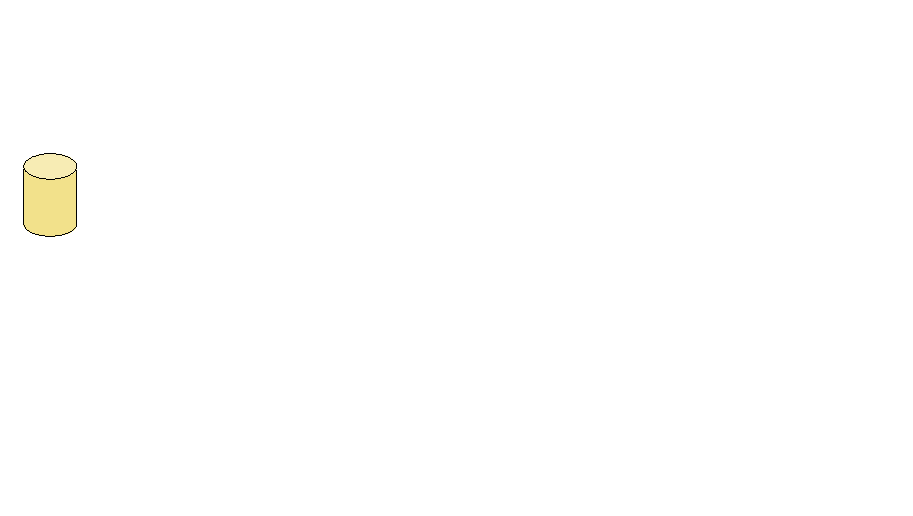
\includegraphics[width=\textwidth]{proposed_architecture.eps}
		\caption{Proposed Architecture}%
		\label{fig:proposed_architecture}
	\end{figure}

	The software architecture will probably be developed in C++, but other
	languages such as Python may also be employed. The following lists the main
	design goals of the proposed architecture:

	\begin{enumerate}

		\item\label{goal:flexibile}

			Be flexible and extendible.

		\item\label{goal:guarantee_trajectory}

			Guarantee collision free trajectories.

	\end{enumerate}

	Goal~\ref{goal:flexibile} may be achieved by adhering to good coding
	practices, whereas Goal~\ref{goal:guarantee_trajectory} is more algorithmic
	in nature. It requires a good understanding and implementation of algorithms
	and methods such as those reported in this literature study.

	One point that may be worth exploring is the generation of an architecture
	that can adapt to different \gls{cdpr} structures. This will require the
	creation of a configuration file format that describes the topology of the
	robot. This is represented as the ``Robot Topology'' database in
	Figure~\ref{fig:proposed_architecture} and may help to further
	Goal~\ref{goal:flexibile}. Furthermore, the steps denoted in
	Figure~\ref{fig:proposed_architecture} should be designed as separate
	modules that adhere to a predetermined interface. This will enable them to
	be interchanged with other modules and algorithms during the progression of
	the thesis.

	With a knowledge of the topology, the architecture will be capable of
	building an internal representation of the robot. Using a type of
	semi-algebraic representation such as those discussed in
	Section~\ref{sec:semi_algebraic_representation_of_bodies} seems to be the
	most promising at present, but other representations may also be
	investigated. A similar approach can be used to model obstacles in the
	world.

	It may be expensive to evaluate the workspace of the robot using methods
	from Section~\ref{sec:continuous_workspace_determination}, but may be worth
	investigating such an approach. Persisting the workspace representation
	could save time in future calculations. The main potential benefit of
	modelling the workspace is that it could potentially limit the total
	configuration space that needs to be searched for a path.

	$\configurationspace$ should ideally be sampled in such a way as to allow
	multiple queries, thereby improving the overall response time of the
	architecture. To this end, $\configurationspace_{\freeregion}$ will be
	represented in a topological graph $\topologicalgraph$ that can be used with
	classical discrete graph search algorithms. Depending on the path planning
	algorithm used, it might be necessary to smooth the calculated path. This is
	currently envisioned as a step after the path has been calculated and may be
	implemented by following methods similar to that described in
	Section~\ref{sec:smoothing_random_paths}.

	The path generated by the architecture should ideally not yet encode any
	timing of the final trajectory. The ``Generate Trajectory'' step of
	Figure~\ref{fig:proposed_architecture} should instead translate the path
	into a time-dependent trajectory. Methods from
	Chapter~\ref{sec:trajectory_generation} may be used in this step. Finally,
	it may be necessary to employ post-processing methods discussed in
	Section~\ref{sec:trajectory_scaling} to meet dynamic requirements of the
	trajectory.


	\chapter{Collision Detection}%
\label{chap:collision_detection}

	% Part~\ref{part:path_planning_approach} discusses in more detail the path
	% planning approach followed in the current thesis. This chapter discusses the
	% collision detection algorithms used, while later chapters discuss the
	% planning and post processing steps.

	There are several types of collision that may occur in a \glspl{cdpr}. These
	are:

	\begin{enumerate}

		\item Cable-Cable collisions

		\item Cable-Obstacle collisions

		\item Cable-End-Effector collisions

		\item End-Effector-Obstacle collisions

	\end{enumerate}

	The following assumptions were made for the collision-detection
	algorithms:

	\begin{enumerate}

		\item

			Cables are modelled as straight lines. If the tension in the cables
			is sufficiently high, this assumption is satisfied. The current
			collision-detection algorithms make no attempt to detect collisions
			in sagging cables.

		\item

			The end-effector and the obstacles are approximated as convex
			polyhedra. To ensure a safety margin, obstacles are usually modelled
			to be slightly larger than they are in reality. This justifies the
			use of convex  shapes to approximate them. For cases where modelling
			an obstacle as a convex shape is unnecessarily wasteful, a
			non-convex obstacle can be built up out of the union of convex
			obstacles.

		\item

			The capacity
			margin (briefly defined in Section~\ref{sec:capacity_margin})
			is considered in the static case only. Dynamic effects on the
			capacity margin are neglected.

	\end{enumerate}

	The current chapter discusses the algorithms used to detect these classes of
	collisions.

	\section{Cable-Cable Collisions}%
\label{sec:cable_cable_collisions}

	To facilitate collision detection, the cables are modelled as parametric
	lines. As a brief recall, a line $\linevec$ between two points $\point_A$
	and $\point_B$ may be written in parametric form as:

	\begin{equation}
		\linevec = \point_A + \timenorm(\point_B - \point_A)
		\label{eq:parametric_line}
	\end{equation}

	Where $\timenorm \in [0, 1]$.

	To detect whether two cables are in collision, consider
	Figure~\ref{fig:cable_cable_collision_detection}.

	\begin{figure}[hb]
		\centering
		\def\svgwidth{\columnwidth}
		\import{res/img/}{cable_collision_detection.pdf_tex}
		\caption{Cable-Cable Collision Detection}
		\label{fig:cable_cable_collision_detection}
	\end{figure}

	The equations of the cables in the figure are:

	\begin{equation}
		\cable_i = \distalanchor_i + \timenorm_i(\proximalanchor_i -
		\distalanchor_i)
	\end{equation}

	for $i = \{1, 2\}$. Considering for now the two-dimensional case and
	assuming the cables are of infinite length, their intersection point may be
	found by solving:

	\begin{align}
		\cable_1 &= \cable_2 \\
		\distalanchor_1 + \timenorm_1(\proximalanchor_1 - \distalanchor_1) &=
			\distalanchor_2 + \timenorm_2(\proximalanchor_2 - \distalanchor_2)
	\end{align}

	This may be put into matrix form:

	\begin{align}
		\left[
			\begin{matrix}
				\proximalanchor_1 - \distalanchor_1 &
				\distalanchor_2 - \proximalanchor_2
			\end{matrix}
		\right]
		\left[
			\begin{matrix}
				\timenorm_1 \\
				\timenorm_2 \\
			\end{matrix}
		\right]
		&=
		\left[
			\begin{matrix}
				\distalanchor_2 - \distalanchor_1
			\end{matrix}
		\right]
		%
		\\
		%
		\mat{A}\vec{\timenorm} &= \vec{b}%
		\label{eq:cable_cable_interference}
	\end{align}

	In the two-dimensional case, we have that $\dim\mat{A} = 2\times2$ and
	$\dim\vec{\timenorm} = \dim\vec{b} = 2\times1$.
	Equation~\ref{eq:cable_cable_interference} can thus be solved by simply
	taking:

	\begin{equation}
		\vec{\timenorm} = {\mat{A}}^{-1}\vec{b}
	\end{equation}

	Assuming for now zero-width, the cables are in collision if and only if
	$\timenorm_i \in [0, 1]$.

	In the three-dimensional case, infinite lines could lie in different planes.
	This is reflected by the fact that $\dim\mat{A} = 3\times2$,
	$\dim\vec{\timenorm} = 2\times1$ and $\dim\vec{b} = 2\times1$. The system
	can therefore not be solved by taking the inverse of $\mat{A}$. Instead, the
	closest points on the two cables can be found by solving
	Equation~\ref{eq:cable_cable_interference} in the least squares sense:

	\begin{equation}
		\vec{\timenorm} = \pseudoinv{\mat{A}}\vec{b}
	\end{equation}

	Note that this will give the closest points on infinite lines. To find the
	closest points on the finite cables, it is therefore necessary to clamp the
	values in $\vec{\timenorm}$:

	\begin{equation}
		\timenorm_i =
		\begin{cases}
			0, \quad \timenorm_i < 0 \\
			1, \quad \timenorm_i > 1 \\
			\timenorm_i, \quad \text{otherwise}
		\end{cases}
	\end{equation}

	The cables are considered to be in collision if the nearest point is closer
	than some predefined tolerance:

	\begin{equation}
		\norm{\cable_1(\timenorm_1) - \cable_2(\timenorm_2)} < \tol
	\end{equation}

	A safety margin can be ensured by choosing the tolerance sufficiently larger
	than the diameter of a single cable.

	Note that some \gls{cdpr} designs place either the proximal or distal anchor
	of two or more cables at the same point to reduce the risk of
	collision~\cite{bib:cdpr:cable_driven_parallel_robots_theory_and_application}.
	For such cases, cables can be considered collision-free if:

	\begin{equation}
		\timenorm_i = 0 \quad\text{or}\quad \timenorm_i = 1
	\end{equation}

	\section{Cable-Obstacle Collisions}%
\label{sec:cable_obstacle_collisions}

	The approach used for cable-obstacle collision detection is based on the
	intersection of parametric lines and parametric planes. Similarly to the
	parametric line in Equation~\ref{eq:parametric_line}, a parametric plane
	$\plane$ through three points $\point_1, \point_2, \point_3$ can be
	expressed as:

	\begin{equation}
		\plane = \point_1 + \timenorm_1(\point_2 - \point_1) +
		\timenorm_2(\point_3 - \point_1)
	\end{equation}

	Where $\tau_1, \tau_2 \in \Re$.

	To detect whether a cable is in collision with an obstacle, consider
	Figure~\ref{fig:cable_obstacle_collision_detection}.

	\begin{figure}[hbt]
		%\missingfigure{Cable Obstacle Collision}
		\centering
		\def\svgwidth{\columnwidth}
		\import{res/img/}{cable_obstacle_collision.pdf_tex}
		\caption{Cable-Obstacle Collision Detection}%
		\label{fig:cable_obstacle_collision_detection}
	\end{figure}

	A convex polyhedron object $\obstacle$ consists of multiple faces,
	${\face}_i$. A cable is in collision with such an object if it intersects
	with any one of these faces.  The following procedure is therefore run for
	every face of the polyhedron.

	To detect a collision between a face and a cable, the face is first
	approximated as an infinite parametric plane through any three vertices
	$\vertex_i$ on the face. The equations for the cable and infinite plane are:

	\begin{align}
		\cable &= \distalanchor + \timenorm_1(\proximalanchor - \distalanchor)\\
		\plane &= \vertex_1 + \timenorm_2(\vertex_2 - \vertex_1) +
		\timenorm_3(\vertex_3 - \vertex_1)
	\end{align}

	Equating the points and manipulating yields the following expressions:

	\begin{align}
		\cable &= \plane
		%%
		\\
		%%
		\left[
			\begin{matrix}
				\proximalanchor - \distalanchor &
				\vertex_1 - \vertex_2 &
				\vertex_1 - \vertex_3
			\end{matrix}
		\right]
		\left[
			\begin{matrix}
				\timenorm_1 \\
				\timenorm_2 \\
				\timenorm_3
			\end{matrix}
		\right]
		&=
		\left[
			\begin{matrix}
				\vertex_1 - \distalanchor
			\end{matrix}
		\right]
		%%
		\\
		%%
		\mat{A}\vec{\timenorm} &= \vec{b}
	\end{align}

	Since $\dim\mat{A} = 3\times3$, $\dim\vec{\timenorm} = 3\times1$ and
	$\dim\vec{b} = 3\times1$, the intersection of an infinite cable with an
	infinite plane is simply:

	\begin{equation}
		\vec{\timenorm} = {\mat{A}}^{-1}\vec{b}
	\end{equation}

	Now, a necessary condition for collision is that:

	\begin{equation}
		\timenorm_1 \in [0, 1]
	\end{equation}

	If $\timenorm_1 \not\in [0,1]$, it means that the finite cable stops before
	hitting the plane. In such a case, the collision detection algorithm may
	return early.

	For the special case where the face of the polyhedron is a rectangle, a
	sufficient condition for collision is $\timenorm_i \in [0, 1], \quad i =
	\{1, 2, 3\}$.  However, in the general case, when $\timenorm_1 \in [0, 1]$,
	it is not sufficient to test that $\timenorm_2,\timenorm_3 \in [0, 1]$. This
	is because the section of the infinite plane $\plane$ described by the range
	$\timenorm_2, \timenorm_3 \in [0, 1]$ is the regular parallelogram defined
	by the vertices $\vertex_1, \vertex_2, \vertex_3$.
	Figure~\ref{fig:point_in_plane} shows a simple example why this is the case.
	As can be seen in the figure, point $\point$ is inside the parametric
	plane $\plane$ described by the vertices $\vertex_1$, $\vertex_2$ and
	$\vertex_3$, even though $\timenorm_3 \not\in [0, 1]$.

	\begin{figure}[hbt]
		%\missingfigure{Cable Obstacle Collision}
		\centering
		\def\svgwidth{\columnwidth}
		\import{res/img/}{point_in_plane.pdf_tex}
		\caption{Point in $\plane$}%
		\label{fig:point_in_plane}
	\end{figure}

	The cable intersects the plane containing the current face of the polyhedron
	at point $\cable(\timenorm_1)$. It is therefore sufficient to check that
	$\cable(\timenorm_1) \in \face_i$. This is done by use of the logical
	predicate in Equation~\ref{eq:collision_point_with_obstacle},
	page~\pageref{eq:collision_point_with_obstacle}.

	The complete condition for collision is then given by:

	\begin{equation}
		\begin{cases}
			\timenorm_1 &\in [0, 1]\\
			\cable(\timenorm_1) &\in \face_i
		\end{cases}
		\quad \forall i \in \{1, \ldots, \norm{\obstacle}\}
		\label{eq:cable_obstacle_collision_condition}
	\end{equation}

	Where the norm denotes the number of faces of the obstacle $\obstacle$.

	\section{Cable-End-Effector Collisions}%
\label{sec:cable_end_effector_collisions}

	Similarly to obstacles, the end-effector $\robot$ is modelled as a convex
	polyhedron. As a result, the same procedure of
	Section~\ref{sec:cable_obstacle_collisions} can be largely applied for this
	case.

	One small difference is that the cables are always touching the
	end-effector. Therefore, simply following the procedure from before would
	result in collisions always being detected. This is avoided by adjusting
	Equation~\ref{eq:cable_obstacle_collision_condition} slightly to obtain:

	\begin{equation}
		\begin{cases}
			\timenorm_1 &\in [0, 1)\\
			\cable(\timenorm_1) &\in \face_i
		\end{cases}
		\quad \forall i \in \{1, \ldots, \norm{\robot}\}
		\label{eq:cable_robot_collision_condition}
	\end{equation}

	\section{End-Effector-Obstacle Collisions}%
\label{sec:end_effector_obstacle_collisions}

	Collisions between the end-effector and obstacles are detected using the
	well-known
	\gls{sat}~\cite{bib:planning:hierarchical_structure_for_rapid_interference_detection}
	theorem. \gls{sat} is not the fastest collision detection algorithm for two
	convex polyhedra. A superior algorithm may be found
	in~\cite{bib:planning:detecting_intersections_between_convex_polyhedra}.
	However, \gls{sat} is considerably simpler to implement. Furthermore, for
	the planning problems addressed by the current thesis, there are few
	obstacles that are modelled in such a way as to have few faces each. Under
	these conditions, \gls{sat} was found to perform sufficiently fast to not
	cause any bottle-neck in the overall architecture.

	For the sake of completeness, the algorithm is briefly described in
	Algorithm~\ref{alg:sat}. Essentially, it looks for a line that passes
	between the objects without intersecting them. It is sufficient to only test
	the normals of the faces of both objects.

	\begin{algorithm}[ht]
		\caption{Separating Axis Theorem Collision
		Detection~\cite{bib:planning:hierarchical_structure_for_rapid_interference_detection}}%
		\label{alg:sat}
		\begin{algorithmic}[1]
			\Procedure{sat}{$\robot$, $\obstacle$}
				\State{}Put the normalised normal $n$ of every face $\face \in \robot\cup\obstacle$ into a queue $\queue$
				\ForAll{$n \in \queue$}
					\ForAll{vertex $\vertex \in \robot$}
						\State{}Project $\vertex$ onto $n$, keeping track of the highest and lowest values
					\EndFor{}
					\ForAll{vertex $\vertex \in \obstacle$}
						\State{}Project $\vertex$ onto $n$, keeping track of the highest and lowest values
					\EndFor{}
					\If{the intervals do not overlap}
						\State{} Return $\code{no\_collision}$
					\EndIf{}
				\EndFor{}
				\State{}Return $\code{collision}$
			\EndProcedure{}
		\end{algorithmic}
	\end{algorithm}

	\section{Capacity Margin}%
\label{sec:capacity_margin}

	In general, the cables of a \gls{cdpr} have upper and lower bounds on their
	tensions. These bounds limit the set of wrenches at the end-effector that
	the cables can support. This set of available wrenches $\setofavwrenches$ is
	also pose-dependent. Furthermore, for a given application, it is possible to
	define a set of required wrenches $\setofreqwrenches$ that the end-effector
	must support. A pose $\pose$ can be considered valid if the set of available
	wrenches contains the set of required wrenches:

	\begin{equation}
		\setofavwrenches \supseteq \setofreqwrenches
		\label{eq:wrench_set_requirement}
	\end{equation}

	The capacity
	margin~\cite{bib:cdpr:measuring_how_well_a_structure_supports_varying_external_wrenches}
	$\capacitymargin$ is a scalar index that measures the
	degree to which Equation~\ref{eq:wrench_set_requirement} is true. It is
	defined such that:

	\begin{align}
		\begin{split}
			\capacitymargin \geq 0, \quad \setofavwrenches \supseteq \setofreqwrenches \\
			\capacitymargin < 0, \quad \text{otherwise}
		\end{split}
	\end{align}

	The capacity margin may be calculated using the hyperplane shifting
	method~\cite{bib:cdpr:on_the_ability_of_a_cable_driven_robot_to_generate_a_prescribed_set_of_wrenches}.

	% The algorithm for calculating the capacity margin was implemented in C++
	% using the hyperplane shifting method described in\todo{ref hyperplane
	% shifting paper}. The reader is referred to \todo{ref paper list} for the
	% algorithms.

	Although the capacity margin does not test for collisions, it is included in
	the collision-detection module. This is because a pose $\pose$ for which
	$\capacitymargin < 0$ cannot support the required wrenches for the current
	application. This implies that the pose should be considered invalid. From a
	planning perspective, a pose which has a negative capacity margin is
	therefore considered to be in collision.

	\section{Overall Collision Detection Algorithm}%
\label{sec:overall_collision_detection_algorithm}

	The collision detection algorithms described in this chapter execute
	quickly. However, since they can potentially be called a few thousand times
	during the initial path search, it is beneficial to organise them in such a
	way that the algorithms that are more likely to detect a collision are
	executed before those that are less likely. This can lead to potential
	speed-ups during the execution  of the code.  The overall meta-algorithm for
	collision detection is reported in
	Algorithm~\ref{alg:overall_collision_detection}.

	\begin{algorithm}[ht]
		\caption{Overall Collision Detection}%
		\label{alg:overall_collision_detection}
		\begin{algorithmic}[1]
			\Procedure{in\_collision}{}
				\ForAll{\cable}
					\ForAll{\obstacle}
						\If{\code{cable\_obstacle\_collision(\cable, \obstacle)}}
							\State{}\code{return true}
						\EndIf{}
					\EndFor{}
				\EndFor{}
				\ForAll{\obstacle}
					\If{\code{endeffector\_obstacle\_collision(\robot, \obstacle)}}
						\State{}\code{return true}
					\EndIf{}
				\EndFor{}
				\ForAll{$\cable_{\indexi}$}
					\ForAll{$\cable_{\indexj} \neq \cable_{\indexi}$}
						\If{$\code{cable\_cable\_collision}(\cable_{\indexi}, \cable_{\indexj})$}
					 		\State{}\code{return true}
						\EndIf{}
					\EndFor{}
				\EndFor{}
				\ForAll{\cable}
					\If{\code{cable\_endeffector\_collision(\cable, \robot)}}
						\State{}\code{return true}
					\EndIf{}
				\EndFor{}
				\State{}$\capacitymargin = \robot(\pose)\code{.capacity\_margin()}$
				\If{$\capacitymargin < 0$}
					\State{}\code{return true}
				\EndIf{}
				\State{}\code{return false}
			\EndProcedure{}
		\end{algorithmic}
	\end{algorithm}


	\chapter{Sampling}%
\label{chap:sampling}

	The designed architecture uses a sampling approach for path planning. Path
	planning was first investigated in two dimensions before generalising to the
	spatial case. The sampling algorithm chosen is a variant
	of the well-known \gls{rrt}
	algorithm~\cite{bib:planning:rapidly-exploring_random_trees_a_new_tool_for_path_planning}.

	\section{Overview of Planning Steps}

		As an initial overview, Figure~\ref{fig:path_planning_in_2d} shows the
		different planning stages for the planar case. The orange shapes
		represent obstacles that must be avoided. The green dot is the start
		pose of the end-effector, and the red dot is its final pose. For
		simplicity, the end-effector is not drawn in these images. The top-left
		image shows the construction of a topological graph representing
		possible collision-free paths of the end-effector. The top-right image
		shows the output of a graph-search to obtain a feasible path after the
		graph has been built. The bottom-left shows the output of several
		post-processing steps that optimise and simplify the found path.
		Finally, the bottom-right image shows the effect of smoothing the
		corners of the simplified path.

		\begin{figure}[htb]
			\centering
				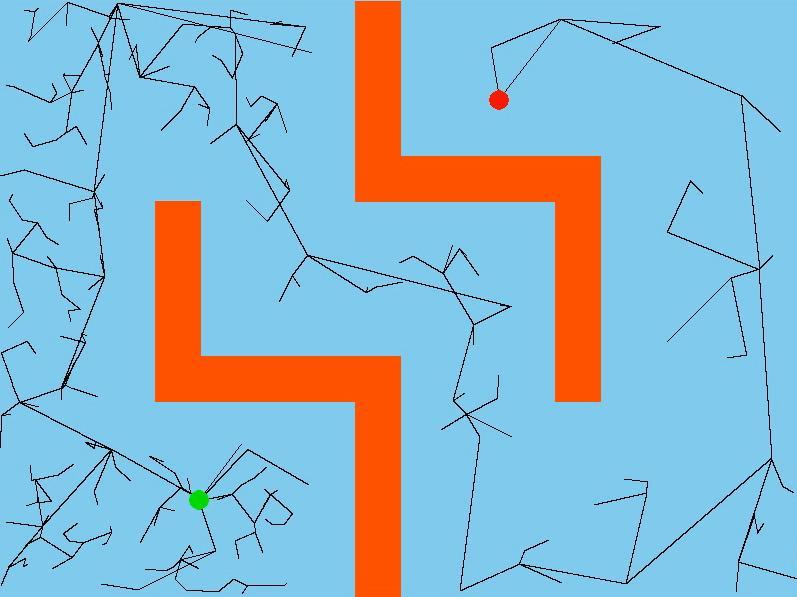
\includegraphics[width=0.45\textwidth]{2d_search_1}%
				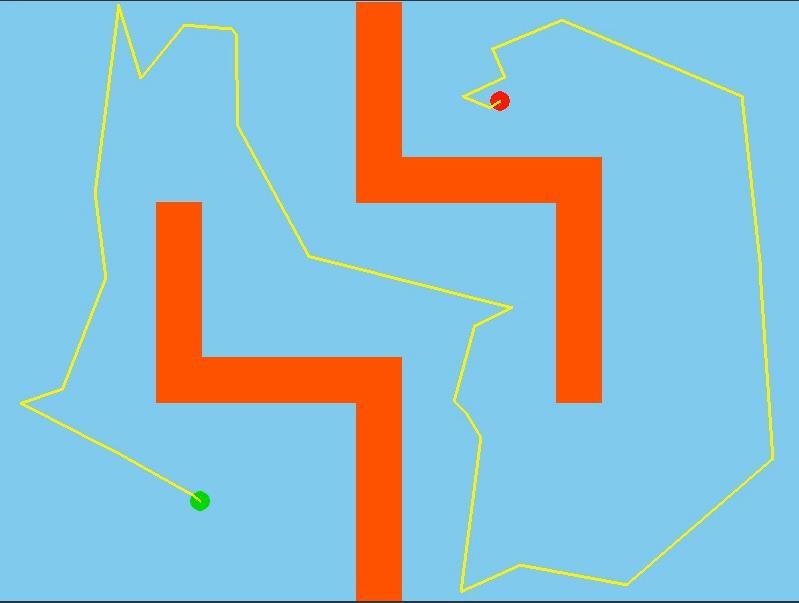
\includegraphics[width=0.45\textwidth]{2d_search_2}\\
				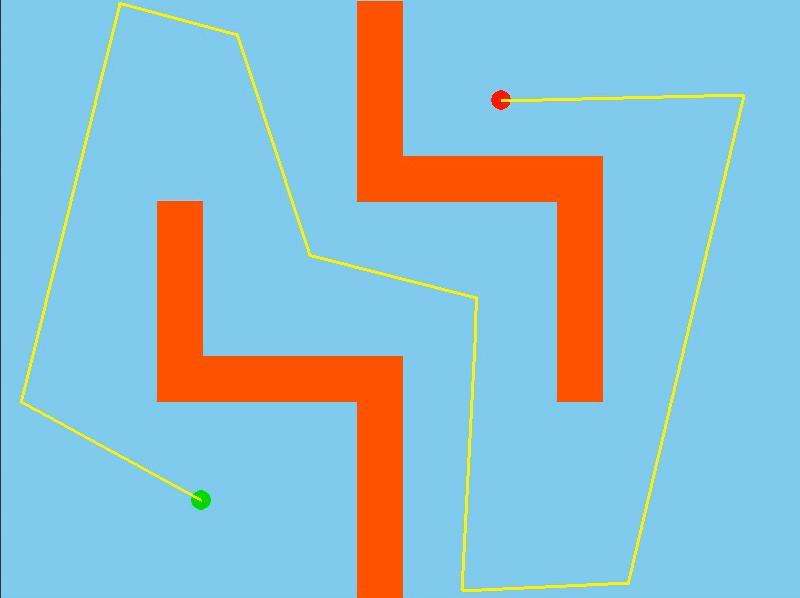
\includegraphics[width=0.45\textwidth]{2d_search_3}%
				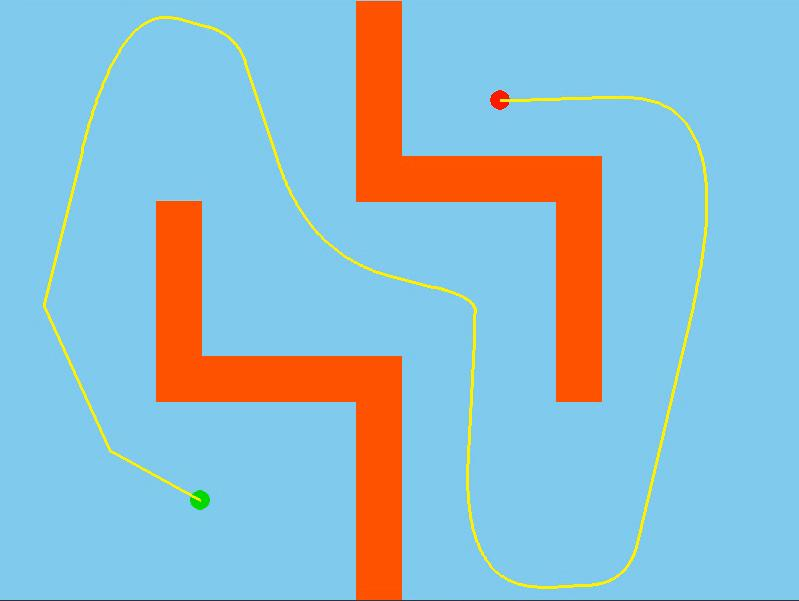
\includegraphics[width=0.45\textwidth]{2d_search_4}
			\caption[Stages of Path Planning]
				{
					Stages of Path Planning\\
					Top Left: Graph Construction,
					Top Right: Graph Search,
					Bottom Left: Path simplification,
					Bottom Right: Path smoothing
				}
			\label{fig:path_planning_in_2d}
		\end{figure}

		The current chapter discusses the generation of the topological graph
		and subsequent graph search represented by the top row of
		Figure~\ref{fig:path_planning_in_2d}. Chapter~\ref{chap:path_processing}
		discusses the post-processing phases corresponding to the bottom row of
		the figure.  Both chapters discuss these procedures for the general case
		in $\specialEuclideanGroup{3}$.

	\section{Sampling Algorithm Overview}%
\label{sec:algorithm_overview}

	% Due to the topology of the class of \gls{cdpr} considered, the sampling
	% algorithm does not need to sample in configuration space, but may instead
	% sample poses directly. This is due to the fact that there is a one-to-one
	% correlation between end-effector pose and robot configuration.

	The first step of the algorithm is to build a topological graph
	$\topologicalgraph$ whose vertices contain collision-free end-effector
	poses. The edges of the graph represent paths between these poses that are
	also free of collision.  After $\topologicalgraph$ is built, a path
	$\pathsym$ is found that connects the start pose $\pose_{\initial}$ to the
	final pose $\pose_{\final}$ by taking into account a custom-defined distance
	function $\dist(\pose_1, \pose_2)$ between two neighbour poses in
	$\topologicalgraph$. A schematic representation is shown in
	Figure~\ref{fig:path_search}. The left side of the figure shows a
	representation of $\topologicalgraph$ in configuration space, whereas the
	right side shows an as-of-yet inefficient path from the start to the goal.

	\begin{figure}[hb]
		\centering
		\def\svgwidth{\columnwidth}
		\import{res/img/}{path_search.pdf_tex}
		\caption{Initial Path Search}%
		\label{fig:path_search}
	\end{figure}


	The pose $\pose$ of the robot $\robot$ is described as a translation
	vector $\transvec$ combined with a quaternion $\quaternion$:

	\begin{equation}
		\pose = (\transvec, \quaternion)
	\end{equation}

	Furthermore, the algorithm defines a graph $\topologicalgraph$ of poses.
	During each iteration, the algorithm samples a new pose,
	$\pose_{\indexi}$ such that:

	\begin{equation}
		\robot(\pose_{\indexi}) \not\in
		\configurationspace_{\obstacleregion}
	\end{equation}

	and attempts to add it to the graph:

	\begin{equation}
		\topologicalgraph_{\indexi + 1} \leftarrow
			\topologicalgraph_{\indexi} \cup \pose_{\indexi}
	\end{equation}

	in such a way that:

	\begin{equation}
		\exists \pose_{\indexj} \in \topologicalgraph_{\indexi}
			\quad\suchthat\quad
			\vecline{\pose_{\indexi}}{\pose_{\indexj}} \notin
			\configurationspace_{\obstacleregion}
	\end{equation}

	This last line states that the new sampled pose may be connected to some
	other pose already in the graph in such a way that the path connecting
	the two poses is free of collisions.

	At the same time, at each iteration, the algorithm attempts to add the
	goal pose $\pose_{\goal}$ to $\topologicalgraph$. If this is
	successfully executed, then a path has been found and the algorithm
	terminates. A high-level overview of the algorithm can be found in
	Algorithm~\ref{alg:sampling_planning_overview}.

	\begin{algorithm}[ht]
		\caption{Sampling Planning Overview}%
		\label{alg:sampling_planning_overview}
		\begin{algorithmic}[1]
			\Procedure{Sample\_Search}{$\robot, \obstacle_1, \ldots, \obstacle_n$}
				\State{}$\topologicalgraph = \emptyset \cup \pose_{\initial}$
				\While{$\pose_{\goal} \notin \topologicalgraph$}
					\Repeat{}
						\State{}$\pose_\text{sampled} \leftarrow
						\code{sample\_pose}$\label{alg:sampling_planning_overview:sample_pose}
					\Until{$\robot(\pose) \notin \configurationspace_{\obstacleregion}$}
					\State{}
						\(
							\pose_{\text{neighbour}} =
							\argmin_{\pose_{\indexi} \in
							\topologicalgraph}\dist(\pose_\text{sampled}, \pose_{\indexi})
						\)
					\State{}$\pose_\text{new} =
						\code{farthest\_collision\_free\_point}(\pose_{\text{sampled}},
						\pose_{\text{neighbour}})$\label{alg:sampling_planning_overview:farthest_collision_free_point_sampled}
					\State{}$\code{connect}(\pose_\text{neighbour},
						\pose_\text{new})$
					\State{}$\pose_\text{new} =
						\code{farthest\_collision\_free\_point}(\pose_{\text{new}},
						\pose_{\text{\goal}})$\label{alg:sampling_planning_overview:farthest_collision_free_point_goal}
					\If{$\pose_\text{new} == \pose_{\goal}$}
						\State{}$\code{connect}(\pose_{\goal},
							\pose_\text{new})$
					\EndIf{}
				\EndWhile{}
			\EndProcedure{}
		\end{algorithmic}
	\end{algorithm}

	\section{Sample Strategy}%
\label{sec:sample_strategy}

	Line~\ref{alg:sampling_planning_overview:sample_pose} of
	Algorithm~\ref{alg:sampling_planning_overview} samples a pose from the
	configuration space of the robot in the following manner:

	\begin{enumerate}

		\item

			A translation vector $\transvec$ is drawn from a normal
			distribution such that:
			\label{item:sample_strategy:translation}

			\begin{enumerate}

				\item

					The median of the distribution is the centre of the
					workspace.

				\item

					The edges of the workspace are three standard deviations
					away from the median.
			\end{enumerate}

		\item

			An angle $\theta$ is drawn from a normal distribution with
			median $\pi/2$ and standard deviation $\pi/6$.

			\label{item:sample_strategy:angle}

		\item

			A quaternion is built from the formula:

			\begin{equation}
				\quaternion = 0\vec{i} + \sin(\theta/2)\vec{j} + 0\vec{k} +
					\cos(\theta/2)
			\end{equation}

			\label{item:sample_strategy:quaternion}

			%This produces a rotation of angle $\theta$ around the $y$
			%axis.\todo{explain that y axis is pointing up}

		\item

			The pose $\pose = (\transvec, \quaternion)$ is returned.

	\end{enumerate}

	\subsection{Justification of Sampling Strategy}%
	\label{sec:justification_of_sampling_strategy}

		\glspl{cdpr} are more likely to have a higher capacity margin towards
		the centre of their workspace. This led to the decision to use a normal
		distribution to sample translations as described in
		Item~\ref{item:sample_strategy:translation} above. In doing so, the
		sampling algorithm has a higher probability to choose translations
		closer to the centre of the workspace, thereby increasing the average
		stability of the trajectory found.

		Items~\ref{item:sample_strategy:angle}
		and~\ref{item:sample_strategy:quaternion} in the list above generate a
		rotation $\theta$ around the $y$-axis. The reason that rotations are
		only drawn around the $y$ axis is two-fold. The first reason is that
		experimentation has shown that the architecture performs faster when
		only drawing rotations around a single axis. This is because, by
		removing two rotational axes, the search space is reduced by two
		dimensions. The second reason is that, by only drawing rotations around
		the $y$ axis, the robot is guaranteed to be upright during its
		trajectory. This produces simpler trajectories, as generating completely
		random quaternions would have the robot change its orientation
		unpredictably.

		The mean and standard deviation as defined in
		Item~\ref{item:sample_strategy:angle} are chosen such that 99.7\% of
		the sampled rotations lie within the range $\theta \in [0, \pi]$.
		The effect of using a uniform distribution within this range instead
		of the distribution of Item~\ref{item:sample_strategy:angle} was
		also investigated. This, however, was deemed an inefficient
		approach, as the end-effector was found to have a tendency to
		unnecessarily swing back and forth around the $y$-axis as it
		progressed through its trajectory. By instead biassing the
		end-effector's orientation towards a certain median position, the
		need for a post-processing operation to simplify the orientation's
		progression was significantly reduced.

		Following this approach, given an arbitrary start and end pose, the
		architecture finds a path through several poses in such a way that,
		while moving from the start pose to the first sampled pose, the
		robot is turned upright. Then, while in the middle of its
		trajectory, the robot stays upright. Finally, as the robot
		approaches its final pose, it performs any required arbitrary
		rotations to reach the desired goal pose. This is shown
		schematically in Figure~\ref{fig:pose_sampling}.

		\begin{figure}[hb]
			\centering
			\def\svgwidth{\columnwidth}
			\import{res/img/}{pose_sampling.pdf_tex}
			\caption{Pose Sampling}%
			\label{fig:pose_sampling}
		\end{figure}

	\subsection{Improving the Sampled Capacity Margin}%
	\label{sec:improving_the_sampled_capacity_margin}

		While the sampling strategy in
		Algorithm~\ref{alg:sampling_planning_overview} will find a
		collision-free path, the path may be suboptimal in terms of the capacity
		margin. The capacity margin may be improved as part of a post-processing
		step as explained in Section~\ref{sec:increasing_the_capacity_margin}.
		However, relying on pure post-processing can be expensive. A small
		modification to Algorithm~\ref{alg:sampling_planning_overview} is
		therefore proposed here.

		The idea is to sample poses as before, but then immediately after
		Line~\ref{alg:sampling_planning_overview:sample_pose} in
		Algorithm~\ref{alg:sampling_planning_overview} move them in the
		direction of increasing capacity margin $\capacitymargin$ according to:

		\begin{equation}
			\pose \gets \pose +
				\gain\frac
				{%
					\nabla\capacitymargin
				}
				{%
					\norm
					{%
						\nabla\capacitymargin
					}
				}
			\label{eq:improve_sampled_capacity_margin}
		\end{equation}

		This operation is fairly cheap. Therefore, $\gain$ is kept small and
		Equation~\ref{eq:improve_sampled_capacity_margin} is performed
		repeatedly on the sampled pose $\pose$. This can be seen as taking
		random samples from the configuration space, and then ``sliding'' them
		along the curve defining the direction of increasing capacity margin for
		some predefined distance.

		Due to the shape of the capacity margin polytope, if all samples have a
		favourable capacity margin, then the entire path through these poses
		will also have a good capacity margin.


	\section{Path Checking}%
\label{sec:path_checking}

	\begin{sloppypar}

		There is no guarantee that a sampled pose $\pose_\text{sampled}$ can
		be connected directly to its nearest neighbour
		$\pose_\text{neighbour} \in \topologicalgraph$.
		Figure~\ref{fig:nearest_neighbour} shows one such case. In the figure,
		the green dot represents the last sampled pose. There exists no
		straight-line collision-free path from its nearest neighbour, indicated
		by the red line.

		\begin{figure}[hb]
			\centering
			\def\svgwidth{0.75\columnwidth}
			\import{res/img/}{nearest_neighbour.pdf_tex}
			\caption{Invalid nearest neighbour}%
			\label{fig:nearest_neighbour}
		\end{figure}

		For this reason, the calls to
		$\code{farthest\_collision\_free\_point}$ in lines
		Lines~\ref{alg:sampling_planning_overview:farthest_collision_free_point_sampled}
		and~\ref{alg:sampling_planning_overview:farthest_collision_free_point_goal}
		of Algorithm~\ref{alg:sampling_planning_overview} attempt to
		guarantee that there is no collision between these points.

	\end{sloppypar}

	This is done by discretising points between $\pose_\text{neighbour}$ and
	$\pose_\text{sampled}$ in a straight-line fashion and returning the
	point farthest from $\pose_\text{neighbour}$ before any collision is
	detected. This is summarised in
	Algorithm~\ref{alg:farthest_collision_free_point}.

	\begin{algorithm}[ht]
		\caption{Farthest Collision Free Point}%
		\label{alg:farthest_collision_free_point}
		\begin{algorithmic}[1]
			\Procedure{Farthest\_Collision\_Free\_Point}{$\pose_1, \pose_2$}
				\State{}$\code{dist\_to\_travel} = \dist(\pose_1, \pose_2)$
				\State{}$\code{dist\_travelled} = 0$
				\State{}$\pose_\text{intermediate} = \pose_1$
				\State{}$\pose_\text{prev-intermediate} = \pose_1$
				\While{$\code{dist\_travelled} < \code{dist\_to\_travel}$}
					\State{}
						\(
							\pose_\text{intermediate} =
							\pose_1 +
							\code{dist\_travelled}/\code{dist\_to\_travel}
							(
								\pose_2 - \pose_1
							)
						\)
					\If{\robot($\pose_\text{intermediate}) \in \configurationspace_{\obstacleregion}$}
						\State{}$\pose_\text{intermediate} =
							\pose_\text{prev-intermediate}$
						\State{}break
					\EndIf{}
					\State{}$\code{dist\_travelled} =
						\code{dist\_travelled} + \Delta\configuration$
					\State{}$\pose_\text{prev-intermediate} =
						\pose_\text{intermediate}$
				\EndWhile{}
				\If{$\code{dist\_travelled} > \code{dist\_to\_travel}$}
					\State{}return $\pose_2$
				\EndIf{}
				\State{}return $\pose_\text{intermediate}$
			\EndProcedure{}
		\end{algorithmic}
	\end{algorithm}

	The term $\Delta\configuration$ in
	Algorithm~\ref{alg:farthest_collision_free_point} is an increment that
	determines the resolution at which paths are checked. Its value must be
	chosen such that the algorithm executes quickly, but does not jump over
	obstacles. Its value essentially determines a sphere of radius
	$\Delta\configuration$ around every sampled pose $\pose$ within which it
	is not certain if there is a collision or not.

	% This uncertainty is negated by creating virtual obstacles that are
	% larger than the actual obstacles by a value
	% greater than $\Delta\configuration$. That way, if there is a collision
	% in the uncertain points between $\pose_1$ and $\pose_2$, it will be a
	% collision with a virtual obstacle, but not with the real obstacle.
	% \todo{When this is implemented, discuss it better}

	\section{Distance Measure}%
\label{sec:distance_measure}

	Both Algorithm~\ref{alg:sampling_planning_overview}
	and~\ref{alg:farthest_collision_free_point} require to measure the
	distance between two poses, $\dist(\pose_1, \pose_2)$. This poses a
	problem, however, as a pose is a member of the special euclidean group,
	$\pose \in \specialEuclideanGroup{3}$. There is no one way to measure
	distances in this set and an arbitrary measure is often required. There
	is also the problem that the units used for rotations and translations
	differ.

	Several different measures are often used in these cases. One is to
	simply define the distance as the translational distance between two
	poses:

	\begin{equation}
		\dist(\pose_1, \pose_2) =
			\norm{%
				\pose_2.\transvec - \pose_1.\transvec
			}
		\label{eq:euclidean_distance}
	\end{equation}

	\todo{Add radius of gyration discussion here}

	This thesis proposes to instead measure distances in cable-space. This
	has the following advantages:

	\begin{itemize}

		\item

			Dimensionally homogeneous. Since each pose is related directly
			to the length of the cable-space vector, both the translation
			and orientation of a pose can be measured using meters.

		\item

			Direct correlation to actuators. The change in length of the
			cables relates directly to how much the actuators have to act on
			the cables. Using the cable-space vector as a distance measure
			means that the distance exactly encodes the amount of actuation
			required to move from one pose to another.
			\todo{wording}

	\end{itemize}

	The cable-space vector, $\cablelengths$, can be found from the indirect
	geometric model of the \gls{cdpr}:

	\begin{equation}
		\cablelengths = \invgeometricmodel(\pose)
	\end{equation}

	The distance function is then taken as:\todo{make sure this is correct,
	and implement it in the code}

	\begin{equation}
		\dist(\pose_1, \pose_2) =
			\norm{%
				\invgeometricmodel(\pose_2) - \invgeometricmodel(\pose_1)
			}
		\label{eq:distance_measure}
	\end{equation}

	\subsection{Incorporating the Capacity Margin}%
	\label{sec:incorporating_the_capacity_margin}

		It may be useful to include the value of an index, such as the capacity
		margin, in the distance calculation. For such cases
		Equation~\ref{eq:distance_measure} may be modified to obtain:

		\begin{equation}
			\dist_{\pathsym}(\pose_1, \pose_2) =
				-\gain_{\capacitymargin}
				\frac%
				{%
					\int_0^1 \capacitymargin(\pathsym(\timenorm))\der\timenorm
				}
				{%
					%\int_{\pathsym} \der\pose
					\capacitymargin(\pose_2) - \capacitymargin(\pose_1)
				}
				+
				(1 - \gain_{\capacitymargin})
				\norm{%
					\invgeometricmodel(\pose_2) - \invgeometricmodel(\pose_1)
				}
				\label{eq:distance_measure_capcity_margin}
		\end{equation}
		\todo{This has not yet been implemented in code}
		\todo{dimensionally homogeneous?}

		Here
		\(
			\dist_{\pathsym}
		\)
		measures the distance along the path $\pathsym$ and
		\(
			\gain_{\capacitymargin} \in [0, 1]
		\)
		is a weighting factor that weighs the relative importance of the change
		in capacity margin for a longer path to the straight-line distance
		between two poses.

		The negative sign in front of the integral in
		Equation~\ref{eq:distance_measure_capcity_margin} is due to the fact
		that a path for which the capacity margin is higher should be considered
		more advantageous and therefore shorter.

		The integral in Equation~\ref{eq:distance_measure_capcity_margin} is
		expensive to evaluate repeatedly during the path-planning phase. As
		such, it is instead approximated using a...
		\todo{when implemented, flesh out the following paragraph}



%	\chapter{Path Processing}%
\label{chap:path_processing}

	The sampling algorithm (Algorithm~\ref{alg:sampling_planning_overview})
	exits when it manages to attach the goal pose to the graph
	$\topologicalgraph$. At this point, a Dijkstra-search is performed on
	$\topologicalgraph$ to find an ordered set $\setofposes$ of poses $\pose$
	using the distance function in Equation~\ref{eq:distance_measure} as the
	cost-to-go criterion.

	After this step, a collision-free path $\pathsym$ from the start to the goal
	pose may be found by taking points along the convex hull of subsequent
	points in the set $\setofposes$. The issue now becomes that the convex hull
	between two points is a straight line, which means that different segments
	of $\pathsym$ do not blend smoothly. Furthermore, due to the random nature
	of the sampling algorithm, the set $\setofposes$ may contain superfluous
	poses that will cause $\pathsym$ to be unnecessarily complicated. For this
	reason, several post-processing steps were developed and are discussed in
	the current chapter.

	\section{Path Simplification}%
\label{sec:path_simplification}

	A schematic example of the effect on $\pathsym$ of superfluous poses in
	$\setofposes$ can be seen in the left-hand side of
	Figure~\ref{fig:superfluous_poses}. The algorithms discussed here
	transform such a path into something more closely related to the
	right-hand side of the figure.

	Algorithms were developed to:

	\begin{enumerate}

		\item

			Remove unnecessary poses.

		\item

			Remove corners from the path.

		\item

			Reduce the total amount of rotation along the path.

	\end{enumerate}

	\begin{figure}[hb]
		\centering
		\def\svgwidth{\columnwidth}
		\import{res/img/}{superfluous_poses.pdf_tex}
		\caption{Superfluous Pose Removal}%
		\label{fig:superfluous_poses}
	\end{figure}

	\subsection{Pose Removal}%
	\label{sec:pose_removal}

		A simple recursive algorithm was developed to remove poses from
		$\setofposes$. The pseudocode is given in
		Algorithm~\ref{alg:pose_removal}.

		\begin{algorithm}[ht]
			\caption{Pose Removal}
			\label{alg:pose_removal}
			\begin{algorithmic}[1]
				\Procedure{Remove\_Poses}{}
					\State{}\code{simplified = false}
					\For{$\indexi \in [0, |\setofposes| -2]$}
						\If{$\dist(\pose_{\indexi}, \pose_{\indexi+2}) >
						\dist(\pose_{\indexi}, \pose_{\indexi+1})$}%
						\label{alg:pose_removal:distance_check}
							\If{$\code{Farthest\_Collision\_Free\_Point}(\pose_{\indexi},
							\pose_{\indexi+2}) = \pose_{\indexi+2}$}
								\State{}Remove $\pose_{\indexi+1}$ from
								$\setofposes$
								\State{}$\code{simplifed = true}$
							\EndIf{}
						\EndIf{}
					\EndFor{}
					\If{\code{simplified}}
						\State{}\code{Remove\_Poses}
					\EndIf{}
				\EndProcedure{}
			\end{algorithmic}
		\end{algorithm}

		This algorithm simply removes an intermediate pose if the pose
		before and after it in the sequence in $\setofposes$ can be
		connected by a straight line. However, since a Euclidean distance
		measure (Equation~\ref{eq:euclidean_distance}) is not used, a path
		may actually be \textit{shorter} if an additional intermediate point
		is inserted between two points. For this reason, the algorithm only
		removes points if this would reduce the total travelled distance
		of the path. This is achieved by using the distance measure
		(Equation~\ref{eq:distance_measure_capcity_margin}) in
		Line~\ref{alg:pose_removal:distance_check}.

	\subsection{Corner Removal}%
	\label{sec:corner_removal}

		In some instances, a path cannot be shortened by removing a pose
		from $\setofposes$, since the resulting path would be in collision.
		In such cases, the path may often contain a corner that may be far
		away from the rest of the path. Figure~\ref{fig:path_corner} shows
		a schematic example of this case. To deal with this, an algorithm
		was developed to remove such corners.

		\begin{figure}[hb]
			\centering
			\def\svgwidth{\columnwidth}
			\import{res/img/}{corner_removal.pdf_tex}
			\caption{Path Corner}
			\label{fig:path_corner}
		\end{figure}

		The algorithm tries to find the points $\pose_a, \pose_b$ that
		minimises the total distance travelled along the segment:

		\begin{equation}
			(\pose_a, \pose_b) = \argmin
				(
					\dist(\pose_1, \pose_a) +
					\dist(\pose_a, \pose_b) +
					\dist(\pose_b, \pose_3)
				)
		\end{equation}

		Subject to the constraint:

		\begin{equation}
			\forall
				\obstacle
			\forall
			(
				\pose\in
				\convexhull(\pose_1, \pose_a) \cup \convexhull(\pose_a,
				\pose_b) \cup \convexhull(\pose_b, \pose_3)
			)
			\quad\robot(\pose) \cap \obstacle = \emptyset
		\end{equation}

		This is done by writing the convex hull between two poses as a
		parametric line:

		\begin{align}
			\linevec_1 &= \pose_1 + \timenorm_a(\pose_2 - \pose_1)\\
			\linevec_2 &= \pose_3 + \timenorm_b(\pose_2 - \pose_3)\\
		\end{align}

		Now, using a simple linear search on both $\timenorm_a$ and
		$\timenorm_b$, find the minimum values, $\timenorm_a',
		\timenorm_b'$, for which:

		\begin{align}
			\robot(\convexhull(\pose_1, \linevec_2(\timenorm_b))) \cap
				\obstacle = \emptyset\\
			\robot(\convexhull(\pose_3, \linevec_1(\timenorm_a))) \cap
				\obstacle = \emptyset
		\end{align}

		Now, a two-dimensional binary search is performed on $\timenorm_a$
		and $\timenorm_b$ in the ranges:

		\begin{align}
			\timenorm_a \in [\timenorm_a', 1]\\
			\timenorm_b \in [\timenorm_b', 1]
		\end{align}

		Which produce the poses $\pose_a$ and $\pose_b$ which minimises the
		distance expression and satisfies the constraints of the problem.

	\subsection{Rotation Optimisation}%
	\label{sec:rotation_optimisation}

		Due to the rotation sampling strategy employed as discussed in
		Section~\ref{sec:sample_strategy}, the orientations of the end-effector
		throughout its trajectory will be upright and tend to avoid
		unnecessarily large rotations. However, there may still be some residual
		oscillations around the $y$ axis during its motion. For this reason,
		it is worthwhile to employ a rotation optimisation step.

		The rotation optimisation algorithm uses quaternion
		\gls{slerp}~\cite{bib:math:a_compact_differential_formula_for_the_first_derivative_of_a_unit_quaternion_curve}%
		\cite{bib:math:a_general_construction_scheme_for_unit_quaternion_curves_with_simple_high_order_derivatives}.
		It is summarised in Algorithm~\ref{alg:rotation_optimisation}.

		\begin{algorithm}[ht]
			\caption{Rotation Optimisation}
			\label{alg:rotation_optimisation}
			\begin{algorithmic}[1]
				\Procedure{Optimise\_Rotations}{}
					\ForAll{$%
						\pose_{\indexi} \in
							\setofposes\setminus
								(\pose_{\initial}, \pose_{\goal})
					$}
						\State{}%
							$
								\pose_{\indexi}' \gets
									\code{slerp\_interpolate}
									(
										0.5,
										\pose_{\indexi - 1},
										\pose_{\indexi},
										\pose_{\indexi + 1}
									)
							$
							\label{alg:rotation_optimisation:slerp}
						\If{$
							\dist(\pose_{\indexi - 1}, \pose_{\indexi}') +
							\dist(\pose_{\indexi}', \pose_{\indexi + 1})
							\leq
							\dist(\pose_{\indexi - 1}, \pose_{\indexi}) +
							\dist(\pose_{\indexi}, \pose_{\indexi + 1})
						$}
							\If{$
								\code{path\_okay}
									(
										\pose_{\indexi - 1},
										\pose_{\indexi}',
										\pose_{\indexi + 1}
									)
							$}
								\State{}%
									$
										\pose_{\indexi} \gets \pose_{\indexi}'
									$
							\EndIf{}
						\EndIf{}
					\EndFor{}
				\EndProcedure{}
			\end{algorithmic}
		\end{algorithm}

		The algorithm simply iterates over all the poses in the set and attempts
		to adjust the rotation of each pose so that it is between the rotations
		of the poses that precede and follow it. This is done by
		Line~\ref{alg:rotation_optimisation:slerp}, which returns a pose
		$\pose_{\indexi}'$ that has the same translation component as
		$\pose_{\indexi}$, but whose quaternion is the midway point of the
		\gls{slerp} of poses $\pose_{\indexi - 1}$ and $\pose_{\indexi + 1}$.

		The rotation optimisation algorithm could be run multiple times on
		$\setofposes$ to obtain a progressively more linear rotation progression
		from $\pose_{\initial}$ to $\pose_{\goal}$. However, due to the other
		simplification algorithms, the number of poses in $\setofposes$ tends to
		be small and repeated execution is usually not necessary. Furthermore,
		due to the necessity to check collisions, repeatedly running
		Algorithm~\ref{alg:rotation_optimisation} does get expensive quickly.

	\subsection{Increasing the Capacity Margin}%
	\label{sec:increasing_the_capacity_margin}

		At this point a set $\setofposes$ has been found that is guaranteed to
		be collision-free. However, due to the random nature of the path search
		algorithm, little is done to optimise the overall capacity margin
		$\capacitymargin$ of the trajectory. Two approaches to improve the
		capacity margin are proposed:

		\begin{enumerate}

			\item
				Change the condition for the collision detection algorithm.
				\label{option:change_collision_condition}

			\item
				Post-process $\setofposes$ to improve $\capacitymargin$.
				\label{option:post_process_set_of_poses}

		\end{enumerate}

		Option~\ref{option:change_collision_condition} is to define some minimum
		threshold capacity margin ${\capacitymargin}_{\tol}$ and modify the
		capacity margin submodule ${\logicalpredicate}_{\capacitymargin}$ of the
		collision detection algorithm as follows:

		\begin{equation}
			{\logicalpredicate}_{\capacitymargin} =
				\begin{cases}
					\false, \quad \capacitymargin > {\capacitymargin}_{\tol} \\
					\true, \quad \text{otherwise}
				\end{cases}
		\end{equation}

		This will guarantee that at each point in the trajectory the capacity
		margin is above this minimum limit.

		Option~\ref{option:post_process_set_of_poses} requires that each pose be
		changed according to:

		\begin{equation}
			\forall
				\left(
					{\pose}_{\indexi} \neq {\pose}_{\initial}, {\pose}_{\goal}
				\right)
			\in
				\setofposes,
			%
			{\pose}_{\indexi}' \gets
				{\pose}_{\indexi} + {\gain}_{\indexi}\nabla\capacitymargin({\pose}_{\indexi})
			\label{eq:capacity_margin_increase}
		\end{equation}

		Here, the gain ${\gain}_{\indexi}$ determines how far to move
		${\pose}_{\indexi}$ in the direction of increasing $\capacitymargin$. Of
		course, this is subject to the constraints:

		\begin{equation}
			\dist_{\pathsym}
				\left(
					{\pose}_{\indexi - 1},
					{\pose}_{\indexi}'
				\right)
			+
			\dist_{\pathsym}
				\left(
					{\pose}_{\indexi}',
					{\pose}_{\indexi + 1}
				\right)
			<
			\dist_{\pathsym}
				\left(
					{\pose}_{\indexi - 1},
					{\pose}_{\indexi}
				\right)
			+
			\dist_{\pathsym}
				\left(
					{\pose}_{\indexi},
					{\pose}_{\indexi + 1}
				\right)
			\label{eq:constraint_shorter_distance}
		\end{equation}

		and

		\begin{equation}
			\logicalpredicate(\pathsym') = \false
			\label{eq:constraint_no_collision}
		\end{equation}

		These constraints essentially require that the distance found be shorter
		due to an increase in capacity margin, but still be free of collisions.

		Due to the costs involved in evaluating
		Constraint~\ref{eq:constraint_shorter_distance}, the search on
		${\gain}_{\indexi}$ should be limited. As such, it is beneficial to
		define a discrete set ${{\gain}_{\indexi}}_1 \ldots
		{{\gain}_{\indexi}}_n$ for which
		Equation~\ref{eq:capacity_margin_increase} is called.  If this set of
		gains is kept small, the procedure can be run multiple times to search
		for a path with a higher capacity margin. Of course, this has a
		trade-off with the overall calculation time required.

	\section{Smooth Interpolation}%
\label{sec:smooth_interpolation}

	After the path has been simplified using the algorithms described in
	Section~\ref{sec:path_simplification}, a path consisting of straight lines
	with hard corners is obtained. The next step is to generate a smoother
	trajectory that approximates the path while still avoiding obstacles.
	Figure~\ref{fig:path_smoothing} shows a schematic representation of the
	desired output.

	\begin{figure}[hb]
		\centering
		\def\svgwidth{\columnwidth}
		\import{res/img/}{smoothed_path.pdf_tex}
		\caption{Path Smoothing}%
		\label{fig:path_smoothing}
	\end{figure}

	B-spline curves were used to obtain the desired trajectory. To achieve this,
	each pose $\pose$ in the ordered set of poses $\setofposes$ in the
	simplified path is considered as a control point of the final B-spline
	trajectory. The trajectory is then generated using the well-known B-spline
	recursive relation repeated here for
	completeness~\cite{bib:math:spline_notes}:

	\begin{align}
		\begin{split}
			\pathsym(\timesym) &=
				\sum^{|\setofposes|}_{i=0} N_{i, k}(\timesym)\pose_{\indexi}\\
			%%%%
			N_{\indexi, \indexj}(\timesym) &=
				\frac
				{%
					\timesym - \timesym_{\indexi}
				}
				{%
					\timesym_{\indexi + \indexj} - \timesym_{\indexi}
				}
				N_{\indexi, \indexj - 1}
				+
				\frac
				{%
					\timesym_{\indexi + \indexj + 1} - \timesym
				}
				{%
					\timesym_{\indexi + \indexj + 1} - \timesym_{\indexi + 1}
				}
				N_{\indexi + 1, \indexj - 1}\\
			%%%%%
			N_{\indexi, 0}(\timesym) &=
				\begin{cases}
					1, \quad \timesym_{\indexi} \leq \timesym < \timesym_{\indexi + 1}\\
					0, \quad \text{otherwise}
				\end{cases}\\
			%%%%%
			\vec{\timesym} &=
				\left[
					\begin{matrix}
						\timesym_0, \ldots, \timesym_{k + |\setofposes| + 1}
					\end{matrix}
				\right]
		\end{split}
		\label{eq:b_spline_recursion}
	\end{align}

	Where $k$ is the degree of the B-spline used to approximate the points in
	$\setofposes$ and $\vec{\timesym}$ is the equidistant knot vector that
	produces the uniform spline.

	\subsection{Guaranteeing Smooth Path Safety}%
	\label{sec:guaranteeing_smooth_path_safety}

		Blindly applying Equation~\ref{eq:b_spline_recursion} makes no guarantee
		that the smooth path will be collision free. The generated spline curve
		must therefore be checked for collisions and corrective action must be
		taken in the case that a new collision is detected.

		One technique that is commonly used with B-spline curves is that of knot
		multiplicity. The elements in the knot vector $\vec{\timesym}$ are
		generally spaced equidistantly~\cite{bib:math:spline_notes}. However,
		the multiplicity of a knot may be increased by letting consecutive knots
		assume the same value. This has the effect of drawing the spline closer
		to a control point, but also drops a degree of differentiability at this
		point. A schematic representation of this effect can be seen in
		Figure~\ref{fig:knot_multiplicity}.

		\begin{figure}[hb]
			\centering
			\def\svgwidth{\columnwidth}
			\import{res/img/}{knot_multiplicity.pdf_tex}
			\caption{Increased Knot Multiplicity}%
			\label{fig:knot_multiplicity}
		\end{figure}

		While such an approach works, it presents some drawbacks:

		\begin{itemize}

			\item Loss of smoothness.

				A goal of this thesis is to generate smooth trajectories.
				Dropping a degree of differentiability can create
				discontinuities in the jerk, acceleration or velocity profiles
				of the final trajectory. In the worst case, if a point in the
				path degenerates to $\contdeggeom{0}$ --- that is, a hard corner
				in the position profile --- the end-effector would have to come
				to a complete stop at this point and then accelerate from rest
				again. Stopping the motion in the middle of the trajectory is a
				non-ideal approach and should be avoided as much as possible.

			\item Slow Computation Time.

				In general, higher-degree B-spline curves may be used to
				generate a path in configuration space. If part of the curve is
				in collision, then the multiplicity of the point must be
				increased and the path must be checked again. The path can
				potentially still be in collision and, consequently, this
				process can repeat until the offending point degenerates to
				$\contdeggeom{0}$.

		\end{itemize}

		Instead, this thesis proposes to augment $\setofposes$ with additional
		poses such that the spline curve generated from
		Equation~\ref{eq:b_spline_recursion} is guaranteed to be free of
		collisions. This is achieved by noticing from
		Equation~\ref{eq:b_spline_recursion} that any point in $\pathsym$ is
		obtained from convex combinations of subsequent poses. This means that
		the path is guaranteed to go through the convex hull of the currently
		active control points. The consequence of this is that, if the hull of
		the points can be shown to be collision-free, then the path is
		guaranteed to be collision free automatically. The algorithm developed
		is reported in Algorithm~\ref{alg:set_of_poses_augmentation}.

		\begin{algorithm}[ht]
			\caption{$\setofposes$ Augmentation}%
			\label{alg:set_of_poses_augmentation}
			\begin{algorithmic}[1]
				\Procedure{Augment\_Pose\_Set}{\setofposes{}}
					\State{}Declare new set $\setofposes'$
					\State{}Add first pose in $\setofposes$ to $\setofposes'$
					\ForAll{$\pose_{\indexi} \in \setofposes\setminus
					\pose_{\initial}, \pose_{\goal}$}
						\State{}$\pose_0 = \pose_{\indexi - 1}$
						\State{}$\pose_1 = \pose_{\indexi}$
						\State{}$\pose_2 = \pose_{\indexi + 1}$
						\State{}$\timenorm_1 = 0$
						\State{}$\timenorm_2 = 1$
						\While{$\timenorm_1 \leq 0.5$ and $\timenorm_2 \geq 0.5$}
							\State{}$\pose_a = \pose_0 + \timenorm_1(\pose_1 -
								\pose_0)$
							\State{}$\pose_b = \pose_1 + \timenorm_2(\pose_2 -
								\pose_1)$
							\State{}$\timenorm_1 = \timenorm_1 + \Delta\timenorm$
							\State{}$\timenorm_2 = \timenorm_2 - \Delta\timenorm$
							\If{Farthest\_Collision\_Free\_Point($\pose_a, \pose_b)= \pose_b$}
								\State{}break
							\EndIf{}
						\EndWhile
						\State{}$\setofposes'\code{.push}(\pose_a, \pose_1, \pose_b)$
					\EndFor{}
					\State{}Add last point in $\setofposes$ to $\setofposes'$
					\State{}return $\setofposes'$
				\EndProcedure
			\end{algorithmic}
		\end{algorithm}

		A graphical intuition of Algorithm~\ref{alg:set_of_poses_augmentation}
		can be seen in Figure~\ref{fig:set_of_poses_augmentation}. Essentially,
		it tries to find a shorter straight-line path
		$\vecline{\pose_a}{\pose_b}$ that connects poses $\pose_0$ and
		$\pose_2$, but cuts out $\pose_1$. The search is performed by moving
		$\pose_a$ from $\pose_0$ to the midpoint of the line
		$\vecline{\pose_0}{\pose_1}$ and $\pose_b$ from the midpoint of
		$\vecline{\pose_1}{\pose_2}$ to $\pose_1$.

		\begin{figure}[hbt]
			\centering
			\def\svgwidth{0.7\columnwidth}
			\import{res/img/}{subdivide_control_points.pdf_tex}
			\caption{$\setofposes$ Augmentation}%
			\label{fig:set_of_poses_augmentation}
		\end{figure}

		A shorter path could potentially be found by varying $\timenorm_1$ and
		$\timenorm_2$ in nested loops. However, the call to
		\code{Farthest\_Collision\_Free\_Point} is quite expensive. Nested loops
		would mean that the function is called
		\(
			O
			\left(
				\ceil*
				{%
					{%
						\left(
							\frac
							{%
								1
							}
							{%
								2\Delta\timenorm
							}
						\right)
					}^2
				}
			\right)
		\)
		times, instead of just
		\(
			O
			\left(
				\ceil*
				{%
					\left(
						\frac
						{%
							1
						}
						{%
							2\Delta\timenorm
						}
					\right)
				}
			\right)
		\)
		times. Note here that we require $\Delta\timenorm \in (0, 1]$.
		Therefore, the algorithm in its presented state represents a tradeoff
		between speed and path-length.

		A B-spline curve created using Equation~\ref{eq:b_spline_recursion} on
		the augmented set $\setofposes'$ generated from
		Algorithm~\ref{alg:set_of_poses_augmentation} can be viewed as a set of
		straight lines smoothly interpolated with polynomial bends. The
		algorithm has the following benefits:

		\begin{itemize}

			\item Fast

				The algorithm is linear in the amount of times that the
				collision algorithm needs to be called.

			\item Smooth

				The algorithm ensures that sampled points are connected with the
				maximum degree of smoothness that can be achieved by the degree
				chosen for the B-spline curve.
		\end{itemize}

		A schematic representation of the effect of augmenting $\setofposes$ can
		be seen in Figure~\ref{fig:set_of_poses_augmentation_path}. Note that
		although the figure is schematic in nature, it is drawn using B-spline
		curves and control points as discussed in this section.  As can be seen
		in the figure, adding additional control poses $\pose_a$ and $\pose_b$,
		a collision with $\configurationspace_{\obstacleregion}$ can be avoided
		while still maintaining the smoothness of the curve.

		\begin{figure}[hb]
			\centering
			\def\svgwidth{\columnwidth}
			\import{res/img/}{augmented_control_points.pdf_tex}
			\caption{Effecto of $\setofposes$ Augmentation on $\pathsym$}
			\label{fig:set_of_poses_augmentation_path}
		\end{figure}


	\section{Sample Path Processing Output}%
	\label{sec:sample_path_processing_output}


%	\chapter{Motion Law}%
\label{chap:motion_law}

	The path found with the algorithms described in
	Chapter~\ref{chap:path_processing} can be considered as a continuous smooth
	mapping that adheres to:

	\begin{equation}
		\pathsym : \timenorm \in [0, 1] \mapsto \specialEuclideanGroup{3}
			\quad
			\suchthat
			\quad
			\pathsym(0) = \pose_{\initial}, \pathsym(1) = \pose_{\goal},
			\forall\obstacle\forall(\pose\in\pathsym)
				\robot(\pose) \cap \obstacle = \emptyset
	\end{equation}

	If $\timenorm$ is interpreted as time, then it would imply that the robot is
	in its initial pose at $\timesym = 0\si{\second}$ and reaches its goal pose
	at $\timesym = 1\si{\second}$. While $\pathsym$ is guaranteed to be free of
	collisions, this interpretation makes no guarantee that the actuators can
	move the end-effector this fast. For this reason, a motion law,
	$\motionlaw$, must be found that performs the following mapping:

	\begin{equation}
		\motionlaw: \timesym\in\Re \mapsto \timenorm\in[0, 1]
	\end{equation}

	The trajectory, $\traj:\timesym \mapsto \specialEuclideanGroup{3}$, can then
	be defined simply as:

	\begin{equation}
		\traj = \pathsym(\motionlaw(\timesym))
	\end{equation}

	In addition to the no-collision guarantees of $\pathsym$, $\traj$ also
	guarantees that the actuators stay within their saturation ranges. The
	present chapter describes the approach followed to find a suitable
	$\motionlaw$.

	\section{Motion Law Generation Algorithm}%
\label{sec:motion_law_generation_algorithm}

	Since the actuators work directly on the length of the cables, the
	search for a suitable motion law $\motionlaw$ is performed in cable
	space and not in pose space. As a first step, $\timenorm$ is considered
	to be linked directly to time, $\timesym \defeq \timenorm$, and the
	cable velocities along the resulting trajectory is then found as:

	\begin{equation}
		\dot{\cablevec}(\timenorm) =
			\invgeometricmodel
			\left(
				\frac
				{%
					\der\pathsym
				}
				{%
					\der\timesym
				}
			\right)
	\end{equation}

	Each cable in $\cablevec$ is subjected to kinematic constraints on its
	velocity, $\dot\cablelength_{\max}$.  That is, each cable has a maximum
	velocity which it may not exceed. As such, the next step in the algorithm is
	finding the ranges that exceed this maximum velocity. In other words, find
	the set of time instants $\timenorm$ where:

	\begin{equation}
		\abs{\dot{\cablevec}(\timenorm)} \geq \dot{\cablevec}_{\max}
		\label{eq:excessive_cable_velocity}
	\end{equation}

	In general, there may be multiple ranges along the trajectory where the
	maximum velocity in Equation~\ref{eq:excessive_cable_velocity} is
	exceeded. A range in $\timenorm$, $\rangetimenorm$, is encapsulated as
	the ordered tuple:

	%\begin{equation}
	%	\rangetimenorm =
	%		\left(
	%			\timenorm_{\min},
	%			\timenorm_{\max}
	%		\right)
	%	%
	%\end{equation}

	%such that

	%\begin{equation}
	%	\abs
	%	{%
	%		\dot{\cablevec}
	%			(
	%				\timenorm
	%			)
	%	}
	%	%
	%	\geq \dot{\cablevec}_{\max}
	%	\quad
	%	\forall\timenorm\in[\timenorm_{\min}, \timenorm_{\max}]
	%\end{equation}

	%and

	%\begin{align}
	%	\begin{split}
	%		\dot{\cablevec}(\timenorm_{\min}^-) &< \dot{\cablevec}_{\max} \\
	%		\dot{\cablevec}(\timenorm_{\min}^+) &> \dot{\cablevec}_{\max} \\
	%		\dot{\cablevec}(\timenorm_{\max}^-) &> \dot{\cablevec}_{\max} \\
	%		\dot{\cablevec}(\timenorm_{\max}^+) &< \dot{\cablevec}_{\max} \\
	%	\end{split}
	%\end{align}

	\begin{equation}
		\rangetimenorm =
			\left(
				\timenorm_{\min},
				\timenorm_{\max}
			\right)
		%
		\quad
		\suchthat
		\quad
		%
		\begin{cases}
			\abs
			{%
				\dot{\cablevec}
					(
						\timenorm
					)
			}
			\geq \dot{\cablevec}_{\max}
			\forall\timenorm\in[\timenorm_{\min}, \timenorm_{\max}]\\
			%
			\dot{\cablevec}(\timenorm_{\min}^-) < \dot{\cablevec}_{\max} \\
			\dot{\cablevec}(\timenorm_{\min}^+) > \dot{\cablevec}_{\max} \\
			\dot{\cablevec}(\timenorm_{\max}^-) > \dot{\cablevec}_{\max} \\
			\dot{\cablevec}(\timenorm_{\max}^+) < \dot{\cablevec}_{\max} \\
		\end{cases}
	\end{equation}

	Note that the following notation is used to test whether a value is in a
	range:

	\begin{equation}
		\timenorm \in \rangetimenorm =
			\begin{cases}
				\true, \quad \timenorm \in [\timenorm_{\min},
				\timenorm_{\max}] \\
				\false, \quad\text{otherwise}
			\end{cases}
	\end{equation}

	All such ranges are put into an ordered set of ranges,
	$\setofrangestimenorm$, such that:

	\begin{equation}
		{\rangetimenorm}_{\indexi} \prec
		{\rangetimenorm}_{\indexj} \iff
		{\rangetimenorm}_{\indexi}\code{.}{\timenorm_{\max}} <
		{\rangetimenorm}_{\indexj}\code{.}{\timenorm_{\min}}
	\end{equation}

	$\setofrangestimenorm$ is then used as an input to the algorithms that
	generate $\motionlaw$.

	The idea behind the algorithm is now to simply scale the time in such a
	way that:

	\begin{equation}
		\frac
		{%
			\der\timesym
		}
		{%
			\der\timenorm
		}
		=
		\begin{cases}
			1, \quad \timenorm \notin \setofrangestimenorm \\
			\gain_{\indexi}, \quad \timenorm \in {\rangetimenorm}_{\indexi}
		\end{cases}
		\forall{\rangetimenorm}_{\indexi}\in\setofrangestimenorm
	\end{equation}

	Where $\gain_{\indexi}$ is chosen such that, for the currently active
	${\rangetimenorm}_{\indexi}$:

	\begin{equation}
		\abs
		{%
			\dot{\cablevec}(\timenorm)
		}
		\leq \dot{\cablevec}_{\max}
		\quad\forall{\timenorm}\in{\rangetimenorm}_{\indexi}
	\end{equation}

	A graphical intuition of the algorithm is given in
	Figure~\ref{fig:motion_law_graphical_intuition}. The top graph shows the
	velocity profile of a single cable for a given path
	$\pathsym(\timenorm)$. It also highlights the set $\setofrangestimenorm$
	that exceed the maximum velocities. The middle graph shows schematically
	how the motion law $\motionlaw:\timesym \mapsto \timenorm$ is
	generated. Finally, the bottom graph shows the effect of applying
	$\motionlaw$ to $\pathsym$ to obtain a trajectory $\traj(\timesym)$
	which no longer exceeds maximum velocities.

	\begin{figure}[hb]
		\centering
		\def\svgheight{8cm}
		\import{res/img/}{motion_law_intuition.pdf_tex}
		\caption{Motion Law Construction}%
		\label{fig:motion_law_graphical_intuition}
	\end{figure}

	The motion law shown in Figure~\ref{fig:motion_law_graphical_intuition} will
	guarantee that the velocity constraints of the actuators are respected.
	However, the corners in this graph correspond to sudden changes in the rate
	at which $\pathsym$ is followed and can lead to excessive accelerations in
	the cables. For this reason, instead of using the motion law as it is
	presented in Figure~\ref{fig:motion_law_graphical_intuition}, the corners
	are used as control points of the form $\mlcontrolpoint = \left(\timesym,
	\timenorm\right)$. The set of these points is denoted $\mlcontrolpointset$.
	These control points can then be interpolated using a B-spline of sufficient
	degree. A B-spline of degree two can guarantee continuous accelerations.
	Higher-degree B-splines guarantee continuity in higher time derivatives of
	$\traj$. A graphical representation of a B-spline motion law is shown in
	Figure~\ref{fig:motion_law_spline}.

	\begin{figure}[hb]
		\centering
		\def\svgwidth{\textwidth}
		\import{res/img/}{motion_law_spline.pdf_tex}
		\caption{Motion Law B-Spline Interpolation}%
		\label{fig:motion_law_spline}
	\end{figure}

	When interpolating the motion law with a B-spline, certain segments of the
	motion law may have a steeper slope than the corresponding segments of the
	linear interpolation of the control points. A steeper slope means in the
	motion law corresponds to faster progression along the trajectory and
	therefore higher cable velocities than those provided by the base linear
	interpolation.  Figure~\ref{fig:augmented_motion_law_control_points}
	highlights the areas of the motion law of Figure~\ref{fig:motion_law_spline}
	that have a higher slope. These areas correspond to regions where the output
	velocities may violate the constraints. To combat this, the control points
	may be augmented in a manner similar to
	Algorithm~\ref{alg:set_of_poses_augmentation}. The output of this is
	illustrated schematically on the right hand side of
	Figure~\ref{fig:augmented_motion_law_control_points}. The effect of such a
	procedure is to follow the base motion law as closely as possible, but then
	connect the sharp corners with smooth bends.

	\begin{figure}[hb]
		\centering
		\def\svgwidth{\textwidth}
		\import{res/img/}{motion_law_spline_problem.pdf_tex}
		\caption{Augmented Motion Law Control Points}%
		\label{fig:augmented_motion_law_control_points}
	\end{figure}

	There is one issue with using a B-spline in this context, however. Each
	control point for the spline is a coordinate in
	\(
		\left(
			\timesym, \timenorm
		\right)
	\)-space. The B-spline $B$ is a mapping of some variable $x$:

	\begin{equation}
		B: x \in [0, 1] \mapsto \left(\timesym, \timenorm\right)
	\end{equation}

	However, for use with a motion law, an explicit formula of the form

	\begin{equation}
		\timenorm = \timenorm(\timesym)
		\label{eq:direct_relation_motion_law_spline}
	\end{equation}

	is required. To obtain this explicit form, three options are available:

	\begin{enumerate}

		\item

			Rewrite Equation~\ref{eq:b_spline_recursion} in a non-implicit form.
			\label{option:rewrite_non_implicit}

		\item

			Solve for
			\(
				x = \function(\timesym)
			\)
			using numerical techniques such as Newton's method or Regula
			Falsi. Then obtain
			\(
				\timenorm = g(x) = g(\function(\timesym))
			\)
			from there.
			\label{option:solve_numerically}

		\item

			Build a lookup table and smoothly interpolate.
			\label{option:lookup_table}

	\end{enumerate}

	It would clearly be ideal to have a direct relation as in
	Equation~\ref{eq:direct_relation_motion_law_spline}. However,
	Option~\ref{option:rewrite_non_implicit} requires expensive computations and
	difficult to implement algorithms.

	Option~\ref{option:solve_numerically} would require that an implicit
	equation be solved each time the motion law is evaluated. This is not ideal
	when the trajectory is used for robot control.

	For these reasons, this thesis makes uses of the lookup table approach in
	Option~\ref{option:lookup_table}. This is achieved by creating an ordered
	set of pairs

	\begin{equation}
		\set{T} =
		\left\{
			(\timesym_0, \timenorm_0),
			\ldots,
			(\timesym_n, \timenorm_n)
		\right\}
	\end{equation}

	upon creation of the motion law. This is done by defining a discrete set
	$\set{X}$ that spans the domain $x$ of $B$ with
	linearly spaced intervals. $\set{T}$ is then found simply by the relation
	\(
		\set{T} = B(\set{X})
	\).

	The motion law is then approximated by:

	\begin{equation}
		\motionlaw(\timesym) \approx
			\timenorm_{\indexi} +
				\frac
				{%
					\timesym - \timesym_{\indexi}
				}
				{%
					\timesym_{\indexi + 1} - \timesym_{\indexi}
				}
				\left(
					\timenorm_{\indexi + 1} - \timenorm_{\indexi}
				\right)
	\end{equation}

	Where

	\begin{equation}
		\timesym \in [\timesym_{\indexi}, \timesym_{\indexi + 1}]
	\end{equation}

	Using a lookup table did not lead to any noticeable impacts on the
	speed of execution, even when a large number of samples was taken to build
	a high-resolution lookup table. This justifies using the simplification of
	Option~\ref{option:lookup_table} instead of the exactness of
	Option~\ref{option:rewrite_non_implicit}.


	\section{Ensuring a Smooth Start}%
\label{sec:ensuring_a_smooth_start}

	Consider again Figure~\ref{fig:augmented_motion_law_control_points}. The
	algorithm as presented in Section~\ref{sec:motion_law_generation_algorithm}
	will have a tendency to produce infinite accelerations at $\timesym = 0$.
	This is due to the fact that the slope of the B-spline-interpolated motion
	law at $\timesym = 0$ is non-zero and thus represents a loss of
	differentiability analogous to the loss of differentiability in the
	piecewise linear motion law illustrated in the left half of
	Figure~\ref{fig:motion_law_spline}.

	To combat this effect, an acceleration phase may be introduced into the
	motion law. The goal of this phase is to prepend a section that smoothly
	interpolates from zero slope to the initial slope of the original motion
	law. This is done by choosing some acceleration period $\Delta\timesym$ and
	changing the control points according to:

	\begin{equation}
		\timesym_{\indexi} \gets \timesym_{\indexi} + \Delta\timesym
			\quad\forall\timesym_{\indexi} \in \mlcontrolpointset \setminus \timesym_0
	\end{equation}

	This can be seen as shifting all but the first control point further into
	time. Now, a new control point $\mlcontrolpoint'$ must be created subject
	to:

	\begin{align}
		\begin{split}
			\mlcontrolpoint'.\timesym &\in (0, \Delta\timesym)\\
			\mlcontrolpoint'.\timenorm &\in (0, \mlcontrolpoint_1.\timenorm)
		\end{split}
	\end{align}

	$\mlcontrolpoint'$ is then inserted into $\mlcontrolpointset$ between
	$\mlcontrolpoint_0 $ and $\mlcontrolpoint_1$. To ensure that the slope
	during the acceleration phase of the motion law contains a near-horizontal
	section of sufficient length, the following values are used in this thesis:

	\begin{align}
		\begin{split}
			\mlcontrolpoint'.\timesym &= 0.9\Delta\timesym\\
			\mlcontrolpoint'.\timenorm &= 0.1\mlcontrolpoint_1.\timenorm
		\end{split}
	\end{align}

	The effect of applying this procedure is shown schematically in
	Figure~\ref{fig:smooth_start_motion_law_construction}. Although this figure
	intends to give only a graphical intuition, it is drawn using B-spline
	curves. As can be seen in the figure, this procedure effectively shifts the
	entire motion law in time and slowly accelerates the motion law from zero
	slope to its initial slope.

	\begin{figure}[hbt!]
		\centering
		\def\svgwidth{\textwidth}
		\import{res/img/}{acceleration_phase.pdf_tex}
		\caption{Smooth Start Motion Law Construction}%
		\label{fig:smooth_start_motion_law_construction}
	\end{figure}

	\todo{Next section needs to be updated with figures generated using the
	approach of this section}

	\section{Sample Motion Law Processing Output}%
\label{sec:sample_motion_law_processing_output}

	The current section shows and discusses sample output of the algorithm
	described in Section~\ref{sec:motion_law_generation_algorithm}. The current
	discussion relates to the planning problem and trajectory of
	Figure~\ref{fig:motion_law_sample_problem}.

	\begin{figure}[hb]
		\begin{minipage}{0.5\textwidth}
			\centering
			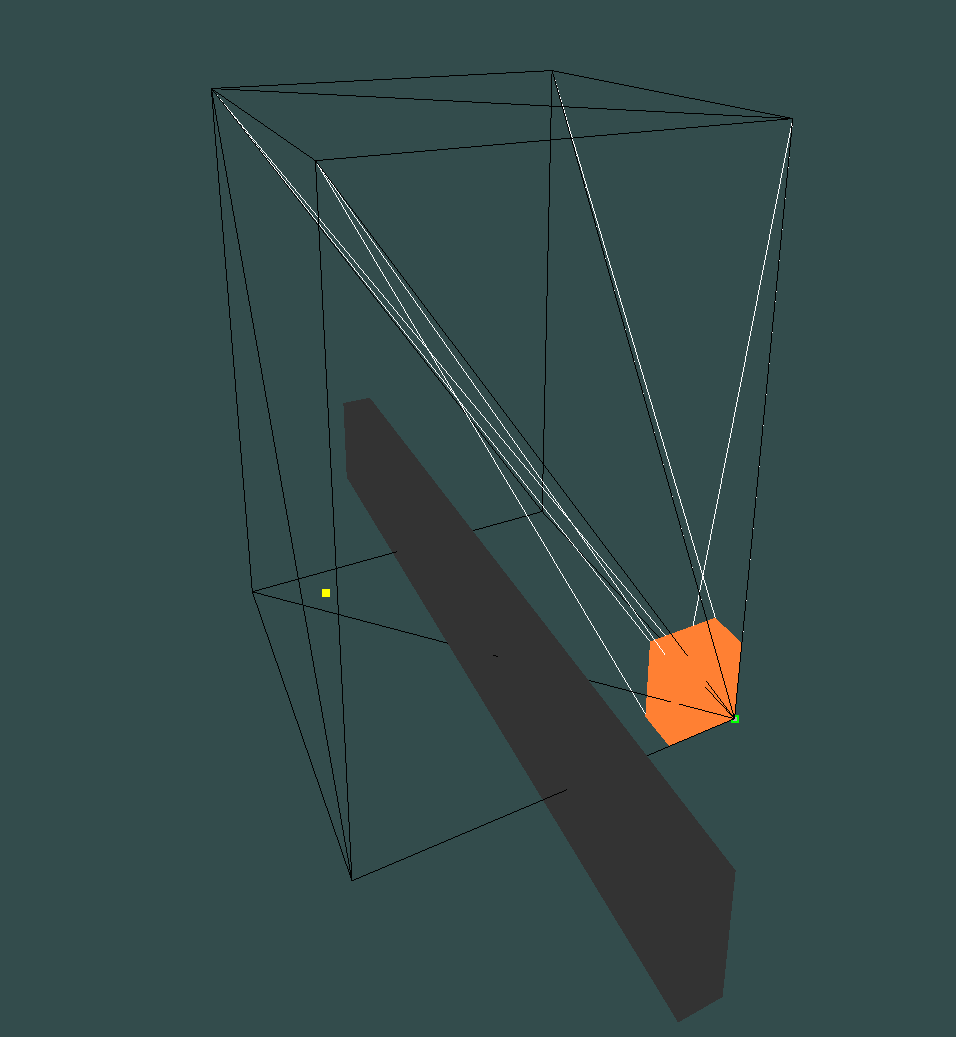
\includegraphics[height=0.6\textwidth]{kinematic_scaling_base_problem}
		\end{minipage}
		\begin{minipage}{0.5\textwidth}
			\centering
			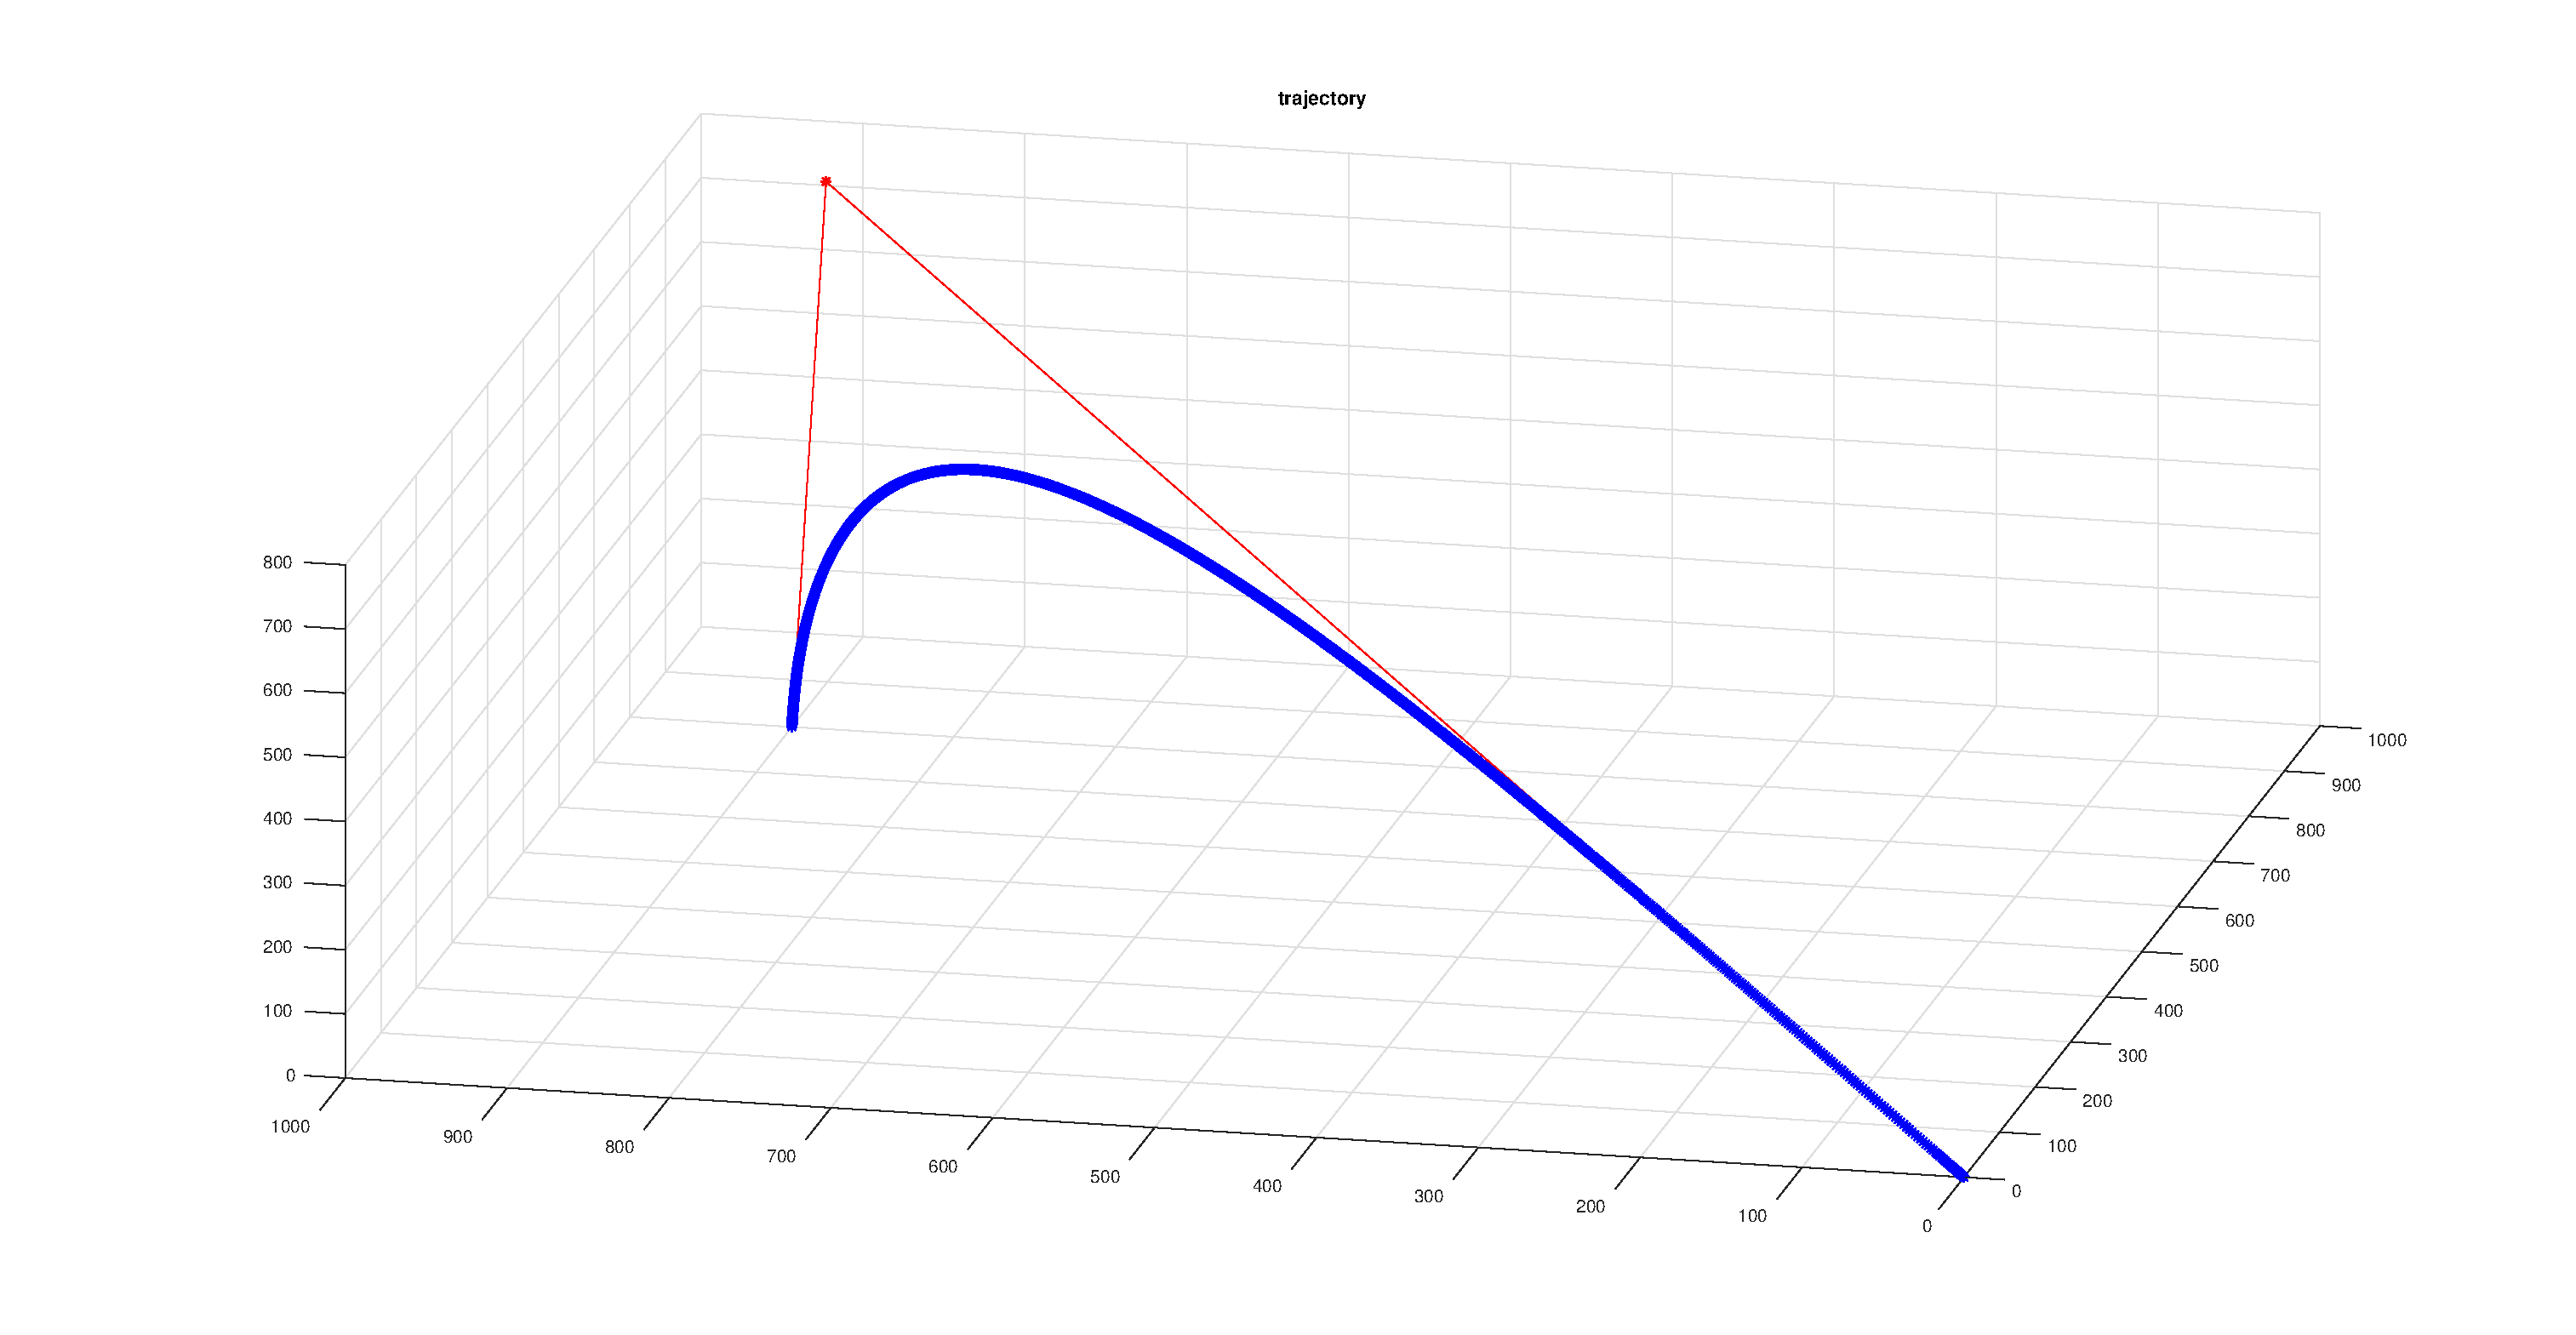
\includegraphics[height=0.6\textwidth]{motion_law_sample_problem_traj}
		\end{minipage}
		\caption[Motion Law Sample Problem]{Motion Law Sample Problem,
		left: problem layout, right: trajectory found}
		\label{fig:motion_law_sample_problem}
	\end{figure}

	\begin{figure}[hbt!]
		\centering
		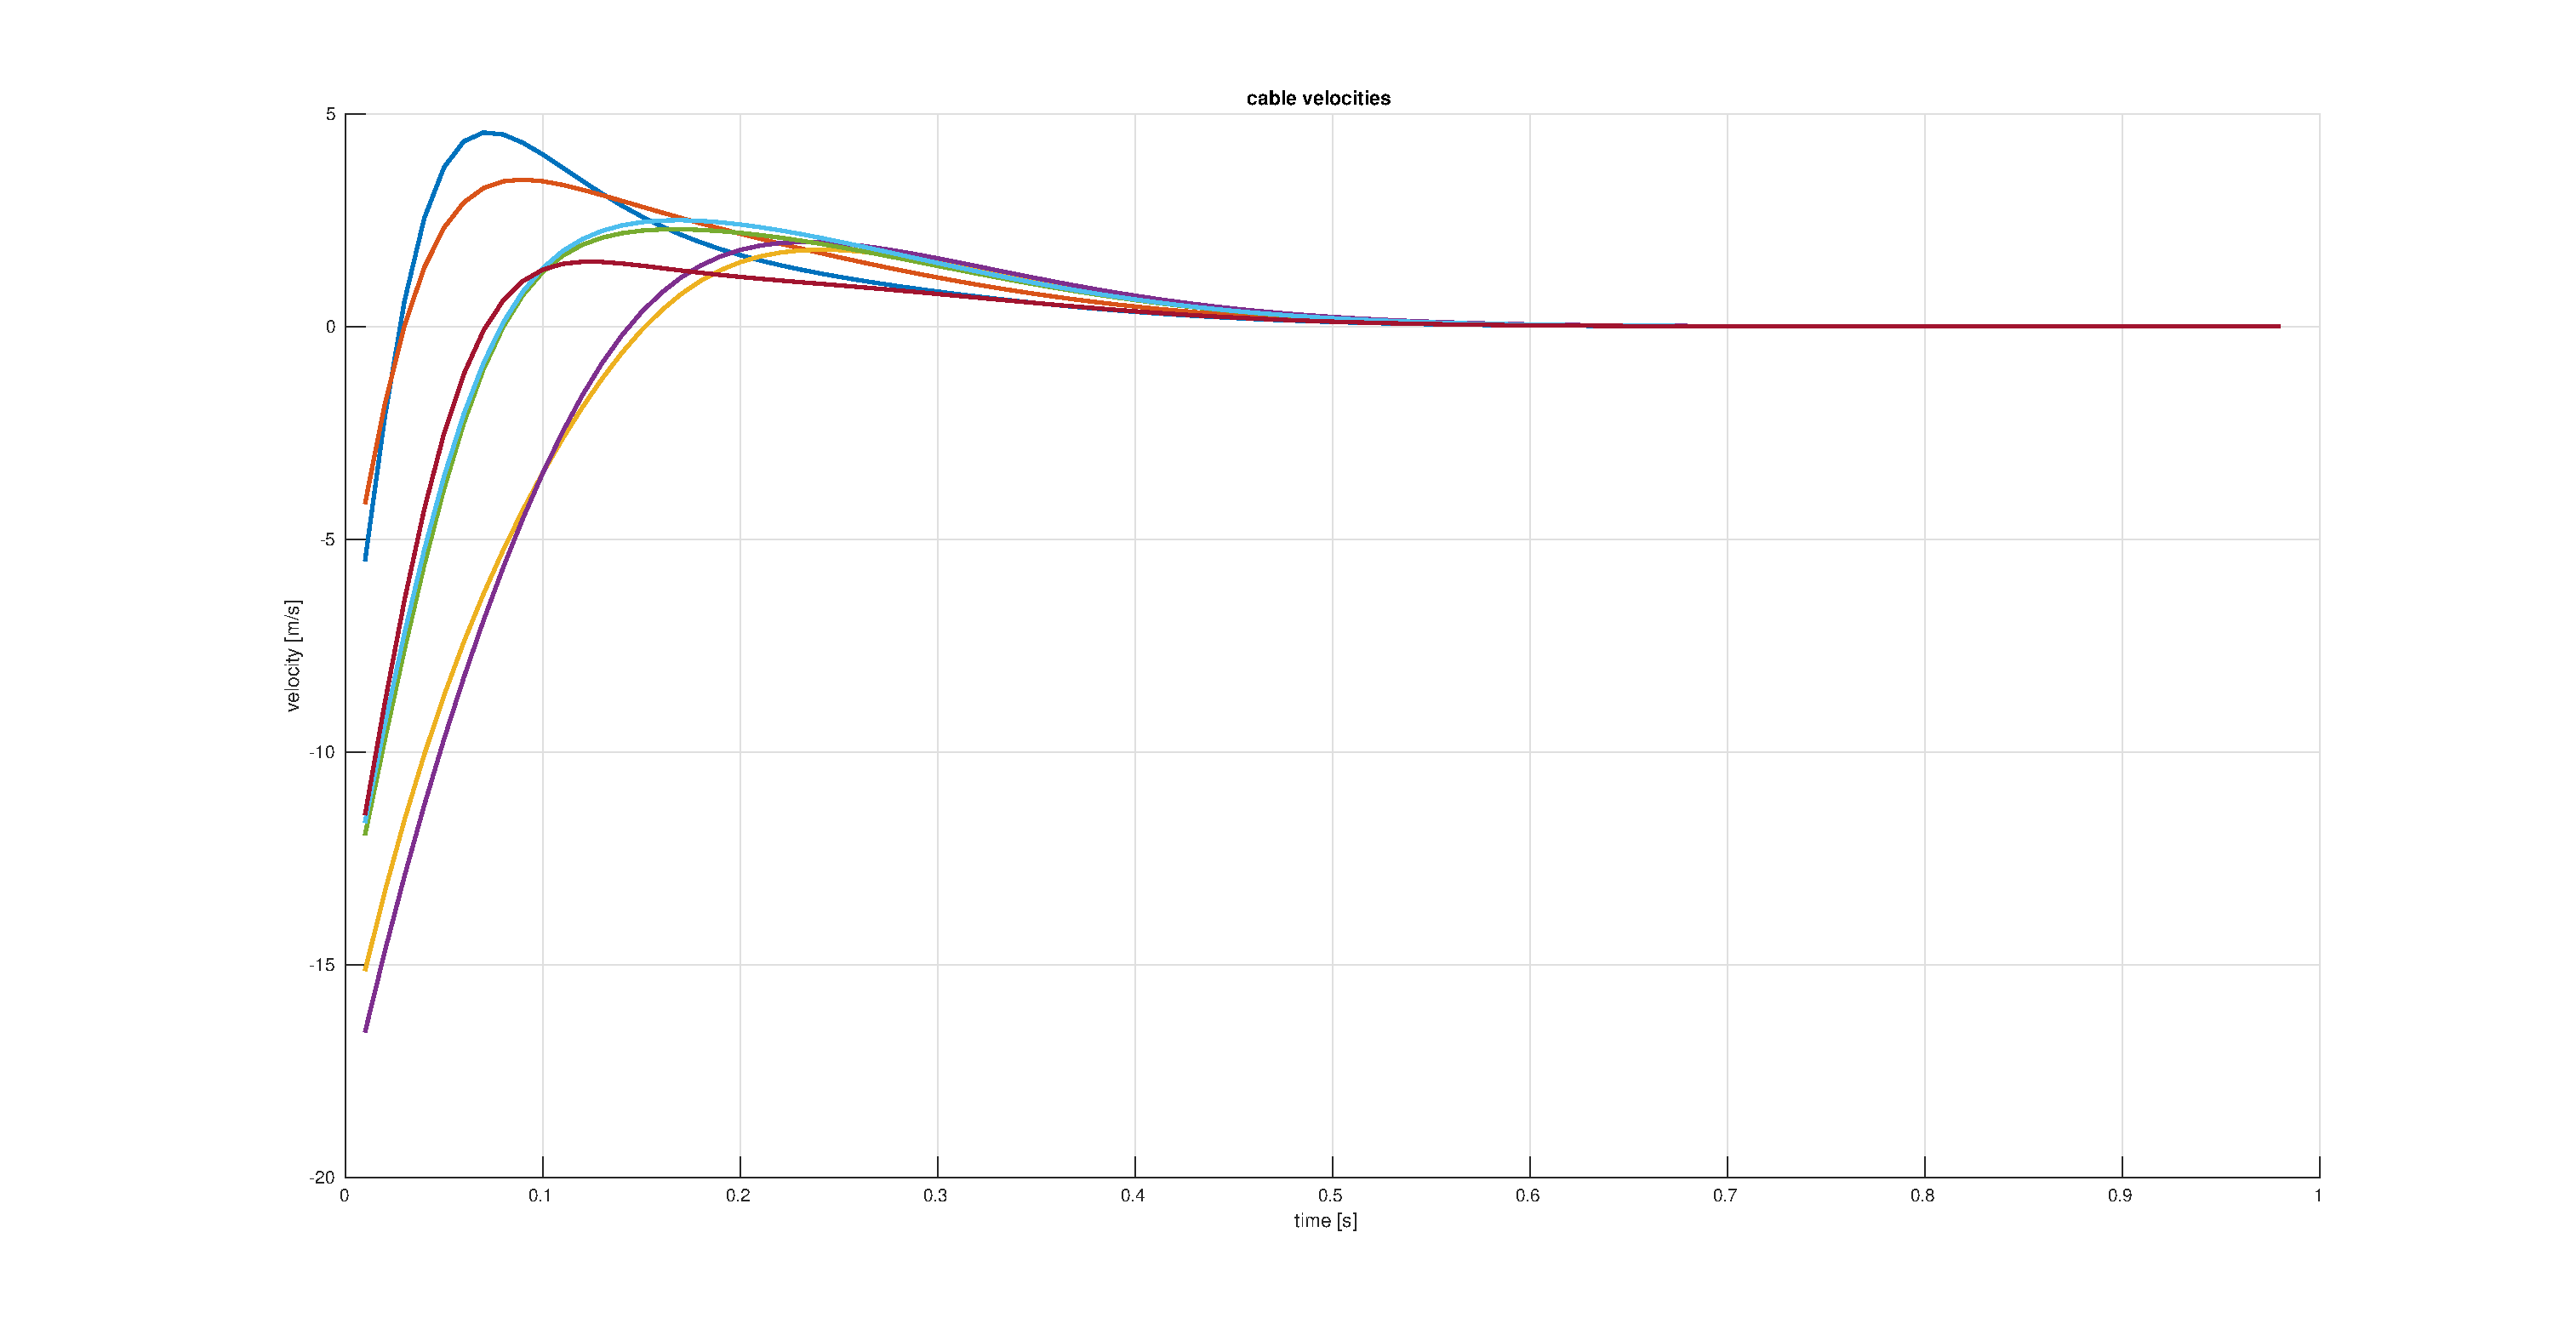
\includegraphics[width=\textwidth]{motion_law_base_velocities}
		\caption{Cable Velocities without Motion Law Scaling}
		\label{fig:cable_velocities_without_motion_law_scaling}
	\end{figure}

	\begin{figure}[hbt!]
		\centering
		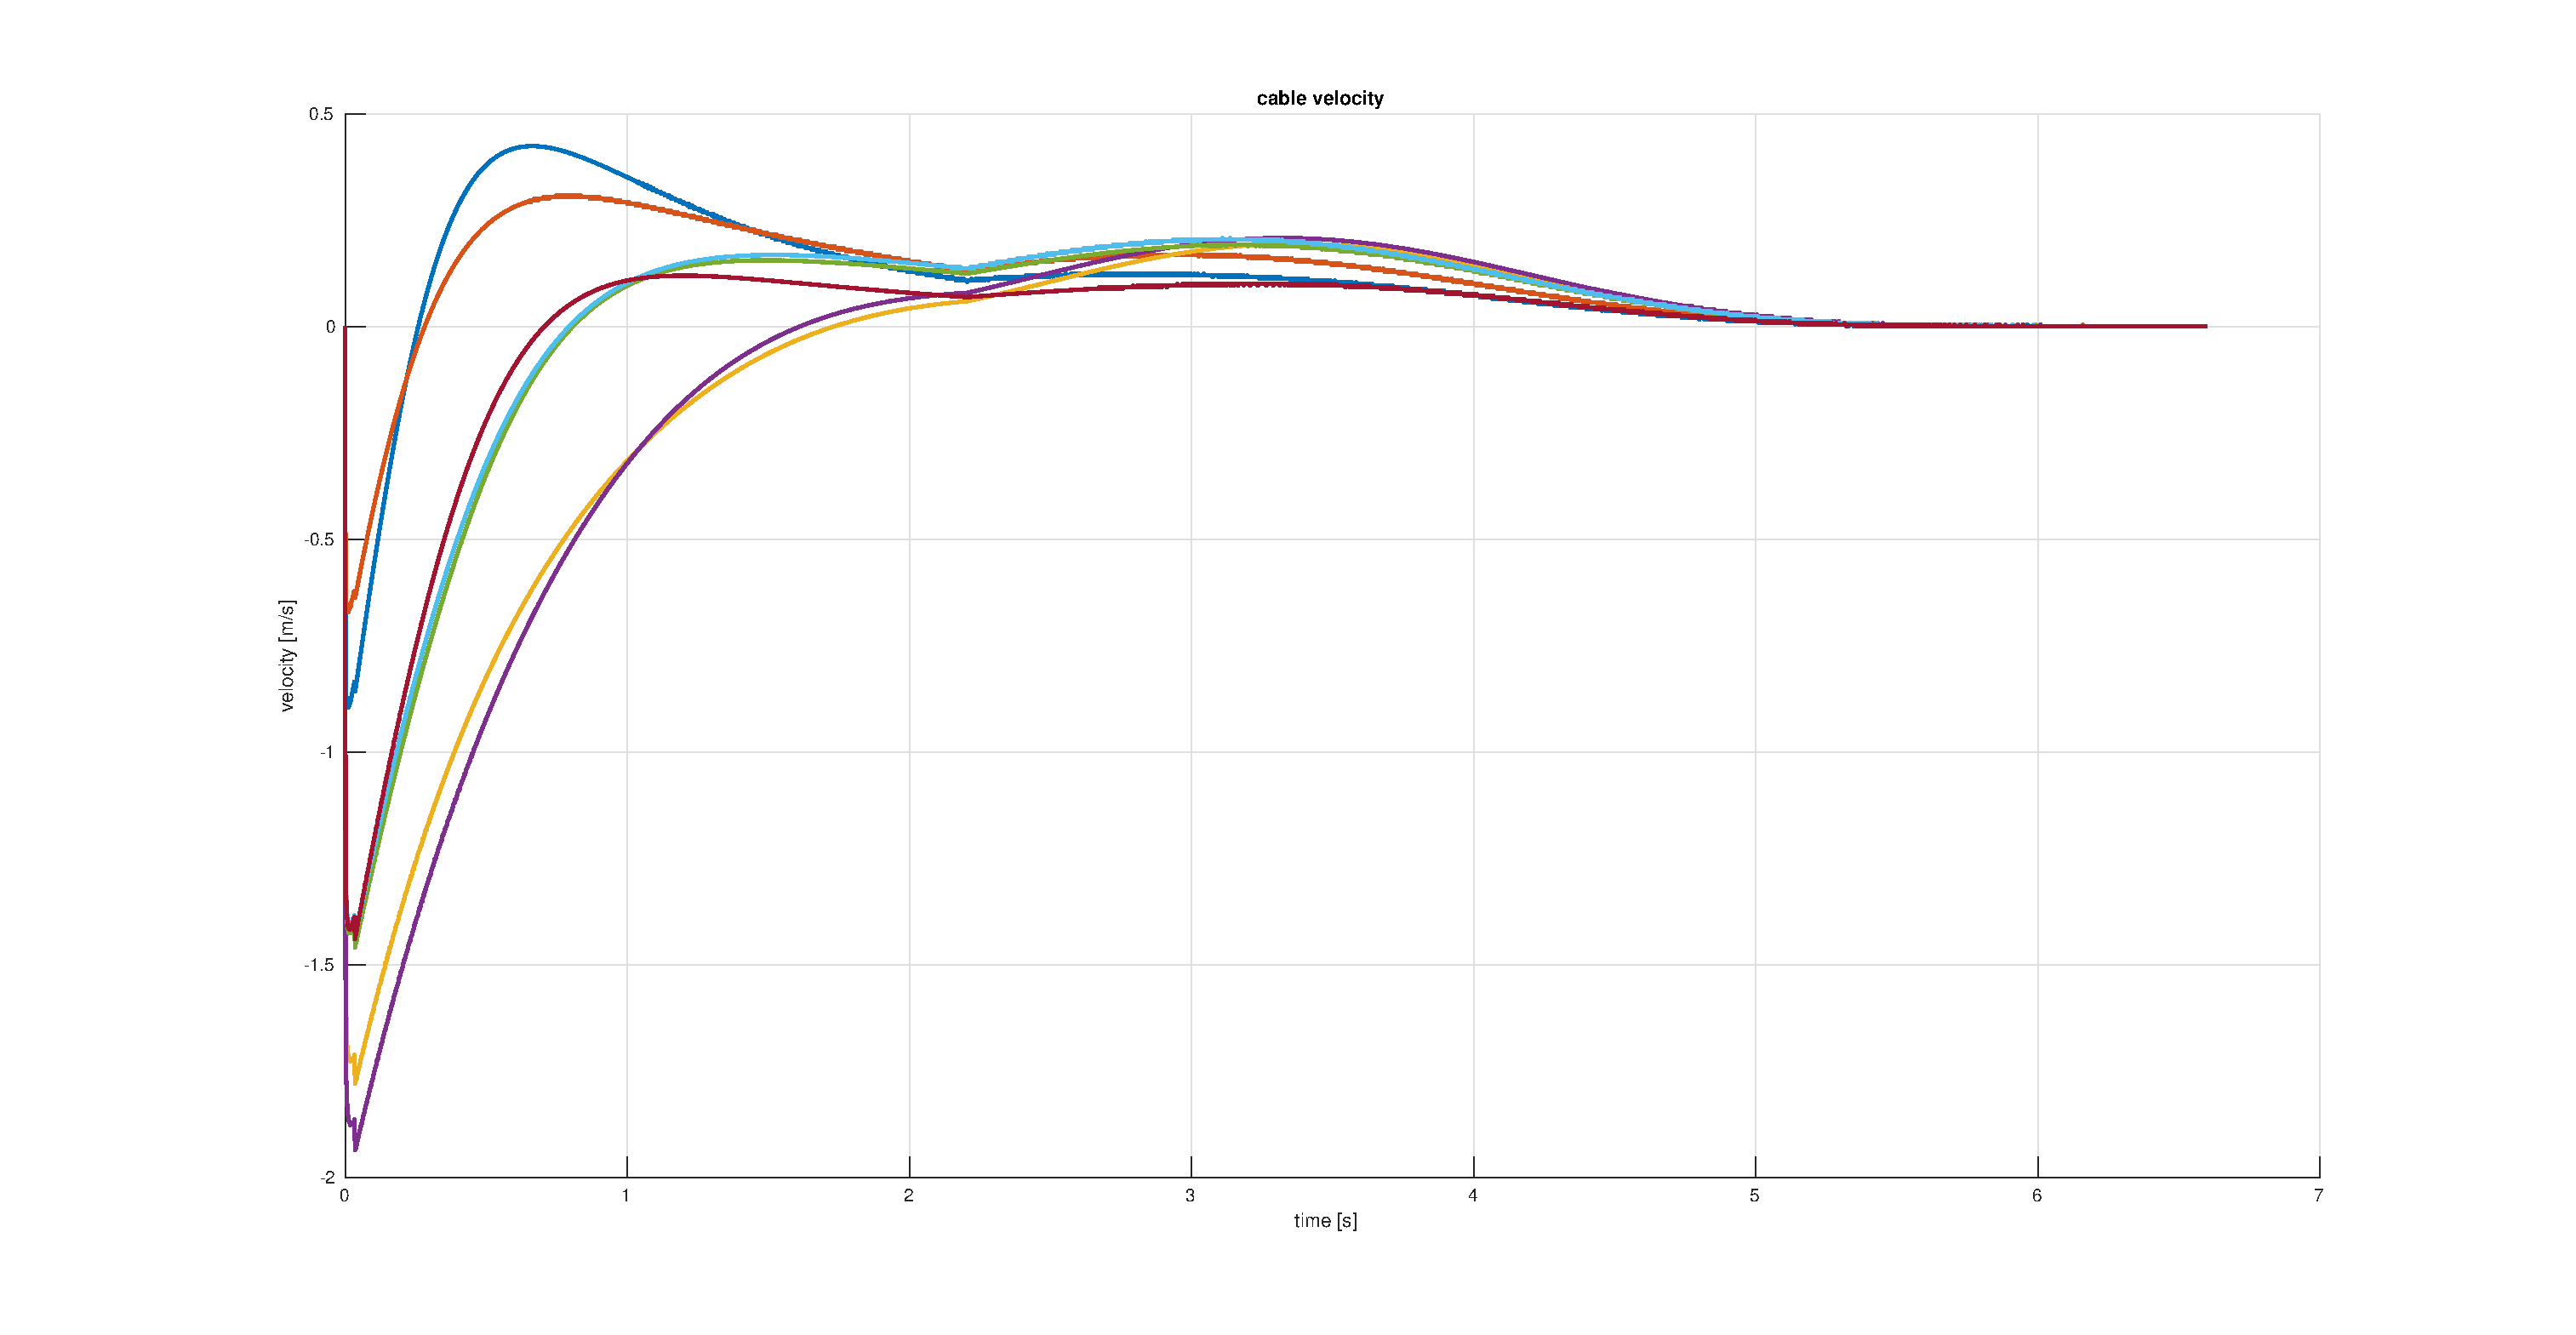
\includegraphics[width=\textwidth]{motion_law_output_velocities}
		\caption{Cable Velocities with Motion Law Scaling}
		\label{fig:cable_velocities_with_motion_law_scaling}
	\end{figure}

	\begin{figure}[hbt!]
		\centering
		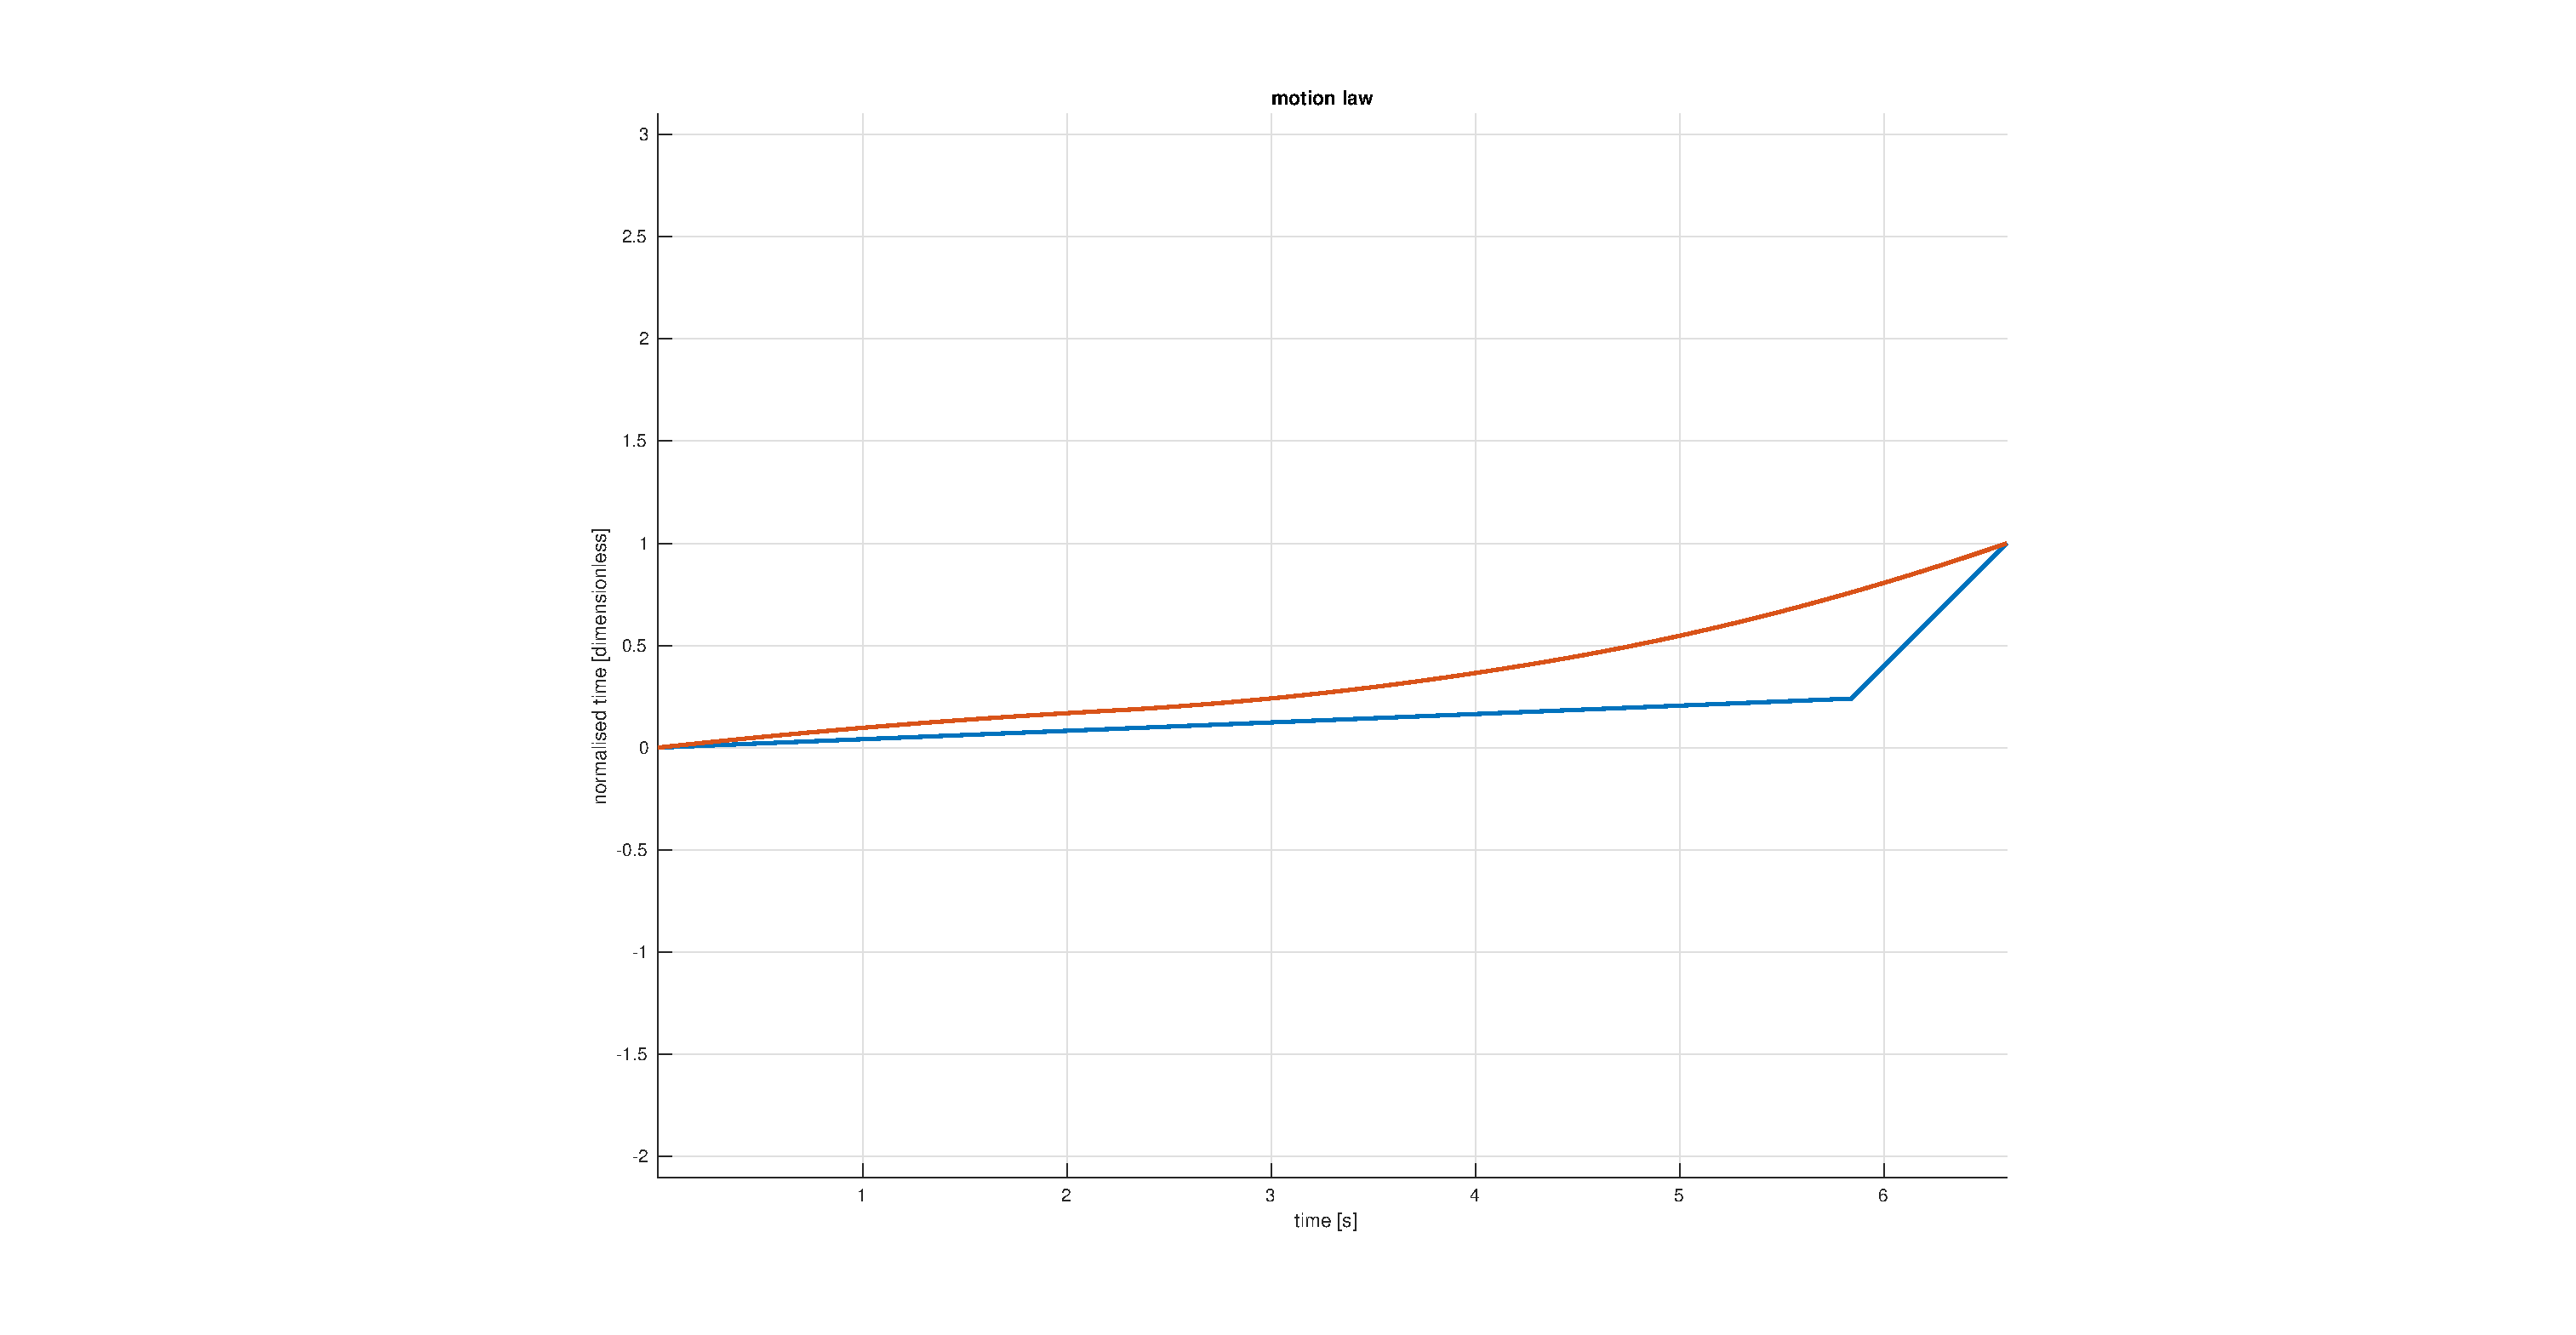
\includegraphics[width=\textwidth]{motion_law}
		\caption{Cable Velocities with Motion Law Scaling}
		\label{fig:motion_law}
	\end{figure}

	The output of the algorithm for this problem is shown in
	Figures~\ref{fig:cable_velocities_without_motion_law_scaling},
	\ref{fig:cable_velocities_with_motion_law_scaling} and~\ref{fig:motion_law}.
	In these figures, the algorithm attempted to find a motion law such that the
	maximum velocity does not exceed $2\si{\meter\per\second}$. For comparison,
	Figure~\ref{fig:cable_velocities_without_motion_law_scaling} shows the case
	where the algorithm is not applied ($\timesym \defeq \timenorm$). As can be
	seen, cable velocities reached up to $15\si{\meter\per\second}$ in this
	case. The motion law generated by the algorithm is reported in
	Figure~\ref{fig:motion_law}. In this figure both the control polygon and the
	B-Spline curve are shown. The output velocities found by applying this
	motion law is shown in
	Figure~\ref{fig:cable_velocities_with_motion_law_scaling}. As can be seen
	from the figurek the motion law succeeds in keeping the cables within their
	velocity bounds.



%
%    \printbibliography{}

\end{document}
